\documentclass[11pt]{article}

\usepackage[margin=1in]{geometry}
\usepackage{amsmath,amssymb}
\usepackage{booktabs}
\usepackage{graphicx}
\usepackage{placeins}
\usepackage[font=small,labelfont=bf]{caption}
\usepackage[colorlinks=true,linkcolor=blue,citecolor=blue,urlcolor=blue]{hyperref}
\usepackage{natbib}
\usepackage{microtype}
\usepackage{xcolor}
\setlength{\emergencystretch}{2.5em}
\captionsetup{skip=5pt}

\newcommand{\stcg}{gated hard with static fallback}
\newcommand{\pelt}{PELT}
\newcommand{\kdyn}{K_{\mathrm{dyn}}}
\newcommand{\kgraph}{K_{\mathrm{graph}}}

\renewcommand{\thesection}{S\arabic{section}}
\renewcommand{\thesubsection}{\thesection.\arabic{subsection}}
\renewcommand{\thetable}{S\arabic{table}}
\renewcommand{\thefigure}{S\arabic{figure}}
\renewcommand{\theequation}{S\arabic{equation}}

\title{Supplementary Material\\[0.6em]
\large State Aggregation in Dynamic Graph Recovery:\\
Separating Structural Ranking from Temporal Discrimination}
\author{Xuansong Chang}
\date{October 2026}

\begin{document}
\maketitle

\paragraph{Evidence guide.}
Sections~\ref{supp:targets}--\ref{supp:derivations} define the targets,
procedures and diagnostic identities. Section~\ref{supp:studies-abc} reports
Studies A--C: A's pre-specified four-contrast family uses $100$ new paired
repeats; B's separately specified schedule comparisons use $50$ different
repeats; C is a separately specified robustness study with $30$ new repeats.
Section~\ref{supp:emission-sensitivity} separates additional controls on existing
outputs from the post hoc AP/threshold and residual-pair sensitivity analysis.
Section~\ref{supp:additional} retains the earlier exploratory grid (seeds
$0$--$19$), a separate auxiliary independent validation (seeds $3000$--$3049$),
representation probes and a fixed segmentation/refit comparison on existing C
inputs. These blocks retain their own statistical units and comparison families.
Section~\ref{supp:industrial} treats static industrial alignment as a separate
reference target. Section~\ref{supp:implementation} distinguishes cached-output
replay from selected same-seed reruns and locates the implementation records.

\FloatBarrier
\section{Evaluation targets and notation}
\label{supp:targets}

\label{sec:problem}

Let $X(1{:}T)\in\mathbb{R}^{T\times N}$ be observed, with latent dynamic state
$z(t)\in\{1,\dots,\kdyn\}$ and directed lag-specific support
$A[k,\ell,i,j]=1$ when $i(t-\ell)$ directly precedes $j(t)$ in state $k$.
For window length $h$ and stride $s$, the window count is
$M=1+\lfloor(T-h)/s\rfloor$, with indices $w=1,\ldots,M$.
Earlier formulas in this supplement use $W$ for the same scalar window count;
there $W=M$. The main article uses $M$ throughout.

\paragraph{Union graph.} $A_{\cup}[\ell,i,j]=1\{\exists k: A[k,\ell,i,j]=1\}$,
scored by AUROC, AUPRC, precision at the true union edge count, and SHD.

\paragraph{Regime-specific graphs.} For each state $k$, the estimated $G[k]$ is
compared with $A[k]$ after matching state identities by maximum overlap. We
report macro AUPRC and AUROC over matched states with non-empty support, the
prevalence of regime edges, the AUPRC lift over prevalence, and the normalized
AP $(\mathrm{AUPRC}-\pi)/(1-\pi)$.

\paragraph{Temporal state sequence.} Window assignments are compared with the
true regime at the window centre, with ARI, macro F1, the signed state-count
error $\hat K-\kdyn$, and state-label boundary F1 at a one-window tolerance.
This earlier label-sequence metric is distinct from the score-change slot
target in Section~\ref{app:direct-localisation}.

\paragraph{Three state counts.} $K_{\mathrm{true}}$ is the number of dynamical
states in the generator, $K_{\mathrm{candidate}}$ is the count handed to a
method, and $\hat K$ is what the method returns. Track~I supplies
$K_{\mathrm{candidate}}=K_{\mathrm{true}}$. A \emph{gate-stress} condition
supplies $K_{\mathrm{candidate}}=2$ when $K_{\mathrm{true}}=1$ on purpose, to
measure false splits. Track~II would supply no count; we define it but do not
claim it as an empirical contribution.

\paragraph{Two structural counts.}
$\kdyn$ counts distinct data-generating mechanisms; $\kgraph$ counts distinct
binary supports. They coincide for a support change or a lag shift, but not for
the mechanism and nuisance families: a sign flip, resampled magnitudes, a
variance change, a mean shift or a state-specific trend produce $\kdyn=2$ with
$\kgraph=1$. When $\kgraph=1$ the regime-specific binary metric -- and likewise
the pooled time-indexed binary target, whose ground truth $A_{z_t}$ is then the
constant graph $A$ -- still scores support recovery but cannot tell whether the
method distinguished the dynamical states; that question is measured by
state-label alignment (ARI) alone. Weighted or signed mechanisms are a third
target that none of the binary metrics evaluates; we report it as a limitation
rather than as a result.

\paragraph{Time-indexed graph scores.}
For an evaluated nonself lagged edge $e$, let $A_{w,e}$ be its support at the
integer centre of window $w$ and $S_{w,e}$ its emitted score. The primary
within-edge temporal AUROC, $\mathrm{T\!-\!AUC}_{\Delta}$, is the macro average
of $\mathrm{AUROC}((A_{w,e})_w,(S_{w,e})_w)$ over edges whose support takes both
values in the evaluation windows. Both positive and negative windows are
required; an undefined target remains missing, while constant scores on an
evaluable edge score $1/2$. Pooled AUROC instead ranks all window--edge entries
together and mixes within-edge and cross-edge comparisons
(Section~\ref{sec:state-factor}). Neither score measures boundary distance.

\paragraph{Distinct recovery questions.}
Boundary detection uses intervals between consecutive window centres. A slot
is positive when an edge's true support changes at least once in that interval;
the predicted change strength is the absolute difference between consecutive
emitted scores. This is change detection at stride resolution. Section~\ref{app:direct-localisation}
defines coverage, AP and threshold conventions.

Binary support is evaluated through union, regime-specific and time-indexed
targets. State assignments are assessed against the centre labels by ARI and
related label metrics; $J$ in Section~\ref{sec:state-factor} specifically denotes
state-assignment discrimination. Score-change boundary detection is defined
separately in Section~\ref{app:direct-localisation}. Signed and weighted mechanism
recovery is not evaluated: the pipeline scores absolute coefficients.
When all states share one binary support, graph scores assess that support
without identifying whether the dynamical states were distinguished.

\FloatBarrier
\section{Generators, local scorers, and comparison procedures}
\label{supp:procedures}

\subsection{Studies A and B: VAR generator and core defaults}
\label{app:config}

Studies A and B share the VAR generator specified below: $N{=}8$ nodes,
$L{=}3$ lags, base edge probability $0.18$, effect scale $1.0$, Gaussian
innovations with scale $0.10$, no observation noise and $100$ burn-in samples.
Their record lengths, duration and schedule conditions vary as specified in
Section~\ref{app:frozen-studies}. Table~\ref{tab:config} collects the reference
scorer and matching settings. Study C uses the separate symmetric construction
in Section~\ref{app:symmetric-sensitivity}.

\paragraph{Coefficient, support and phase construction.}
For each lag, state-$A$ nonself supports are independent Bernoulli draws with
probability $p=0.18$, and all diagonal positions are set to zero.
If the entire tensor is empty, a source $i$ is sampled uniformly from
$\{0,\ldots,N-1\}$ and the lag-one edge $i\to(i+1)\bmod N$ is inserted.
For the support-changing family, state $B$ retains each $A$ edge independently
with probability $o$ (the configured overlap), then adds each position outside
the \emph{original} $A$ support with probability $p(1-o)$.
The addition mask is not recomputed after deleting $A$ edges. Ignoring both
empty-support safeguards, the marginal nonself-edge probability in $B$ is
$po+(1-p)p(1-o)=0.1638$ at $p=0.18,o=0.5$, rather than $0.18$.
If the resulting entire $B$ tensor is empty, it is replaced by the full $A$
support. The
addition mask spans the full tensor, including the initially absent diagonal
slots, so state $B$ can contain self-lag terms. Generated self-lags enter the
VAR recursion and regression design; evaluation and clustering use nonself
entries only. State $A$ has no self terms while state $B$ may have them.
These asymmetric support properties are held fixed in Studies A and B;
Study C evaluates a separate symmetric construction. Before the fallback,
each B diagonal position has probability
$p(1-o)=0.09$. Thus $o$ is a retention probability, not a guaranteed realised
overlap or Jaccard index. Realised
overlap is the shared edge count divided by the state-$A$ edge count. Each
supported coefficient at lag $\ell$ has an independent equiprobable sign and
magnitude $\operatorname{Uniform}(0.08,0.35)\,a/\ell$, where $a$ is effect scale.
Coefficients are resampled in state $B$, including shared edges, except in the
specified identical-coefficient nuisance controls. The sign-flip control uses
the negative of the first-state tensor.

In the two-state branch, a tensor whose initial companion radius $\rho$ exceeds
$0.90$ has every lag block multiplied once by $0.90/\rho$; this is the executed
rescaling rule. For $L>1$ it does not multiply the entire companion matrix by
$0.90/\rho$, and need not make its final radius equal to $0.90$.
It is not a joint-switching stability guarantee. The one-state auxiliary branch
returns its sampled tensor directly. Path stability is assessed separately in
Section~\ref{sec:controlled}. The first $L$ simulation rows are independent
$\mathcal N(0,0.10^2)$ values and later rows follow the VAR recursion with fresh
innovations. The fixed schedule starts in state $A$, alternates after $D$ steps,
and is generated for $T+100$ steps before discarding $100$ burn-in steps.
Consequently observed time zero starts $100$ steps into the original schedule.
This phase convention applies to the fixed-schedule reference; Study B's
random-phase and irregular schedules are specified in Section~\ref{app:frozen-studies}.

\paragraph{Earlier reference configurations.}
The four earlier auxiliary scenarios use $T{=}1200$, window length $h{=}300$,
stride $150$ and $K_{\mathrm{candidate}}{=}2$, with the generator defaults above.
In the switching reference, each state lasts $D{=}300$ steps, the full cycle is
$P{=}600$ and $h=D$. The $100$-step burn-in is not a multiple of $D$, so the
observed switch points fall off the window grid. Scans and control conditions
override these reference settings as specified below.

\begin{table}[!htbp]
\centering
\small
\resizebox{\linewidth}{!}{%
\begin{tabular}{ll}
\toprule
Setting & Value \\
\midrule
Generator & switching VAR(3), $N{=}8$, burn-in $100$; rescaling rule in text \\
Switch schedule & $D{=}300$ per state ($P{=}600$); burn-in $100$ offsets the window grid \\
Coefficient sampling & independent sign $\pm1$, magnitude $U(0.08,0.35)/\ell$ at lag $\ell$ \\
Innovation noise & Gaussian, scale $0.10$; observation noise $0.0$ \\
Scoring & per-variable $z$-score, then Lasso per target on the lagged design \\
Lasso & $\alpha=0.005$ (fixed, not tuned), \texttt{fit\_intercept=False}, \texttt{max\_iter=10000} \\
Design & lag-major: all $L{\times}N$ lagged predictors, both self- and cross-lags \\
Self-lags & fitted in the regression, excluded from edge score and clustering features \\
Standardization & per-variable $z$-score; design and target $z$-scored again before Lasso \\
Clustering features & flattened non-self absolute scores, standardized across windows \\
State assignment & K-means, $K_{\mathrm{candidate}}{=}2$ (gate per Section~\ref{sec:method}) \\
State matching & Hungarian assignment by maximum window overlap (Section~\ref{sec:problem}) \\
Window & $h{=}300$, stride $150$ \\
\bottomrule
\end{tabular}}
\caption{Core simulation defaults for the generator, scorer and state matching;
scans override the stated settings, and ESS has a separate protocol.
``Self-lags'' distinguishes the regression input (self-lags enter the design) from
the edge score and clustering features (self-lag scores are zeroed).}
\label{tab:config}
\end{table}

The four auxiliary scenarios differ only as follows: \emph{switching core}
(\texttt{overlap}{=}0.5), \emph{state-specific} (\texttt{overlap}{=}0.0),
\emph{shared graph} (\texttt{control}{=}\texttt{same\_support},
\texttt{overlap}{=}1.0, second state resampled on the same support), and
\emph{stationary} (\texttt{control}{=}\texttt{stationary}, one state).
Table~\ref{tab:factorial} displays the four configured scenarios using twenty
exploratory seeds per scenario; Table~\ref{tab:aggregation} shows the earlier
switching/stationary panels. The auxiliary independent validation uses fifty
different seeds paired across these same scenario definitions and reports
contrasts after averaging the four scenarios within each seed
(Table~\ref{tab:final}, Section~\ref{supp:aux-independent-validation}).
The exploratory and validation tables therefore describe distinct samples.
The archive retains the full configuration fields.

\subsection{Local scores and hard-emission policies}
\label{sec:method}

We compare emission policies on shared local graph scores. Gated hard uses a static window-maximum output on rejection.
For each window we fit one Lasso per target on lagged standardised inputs and
take absolute coefficients as the window score. Self-lags enter the regression
design but are excluded from the scored edges and clustering features.
Features are the flattened non-self scores, standardised across windows; states
come from K-means with a supplied count. State scores are the within-state mean
of window scores, and the union score is the maximum over state scores.
For time-indexed evaluation, an accepted partition emits its assigned group
map at each window. If the gate rejects, gated hard emits the same
window-maximum map at every window. The
gate accepts when the K-means improvement is at least $0.12$, or when it is at
least $0.04$ with temporal coherence at least $0.55$ and a minimum cluster
fraction at least $0.10$. Improvement is $(I_1-I_K)/I_1$, clipped below at zero,
where $I_1$ and $I_K$ are the one-group and fitted K-means inertias of the
standardised window features; it is set to zero when $I_1\le10^{-8}$.
For the candidate labels before this decision, define empirical group fractions
$f_k=M^{-1}\sum_w\mathbf1(\widehat z_w=k)$, adjacent agreement
$u=(M-1)^{-1}\sum_{w=2}^M\mathbf1(\widehat z_w=\widehat z_{w-1})$ and
$q=\sum_k f_k^2$. The executed coherence is $\max\{0,(u-q)/(1-q)\}$.
It is zero for fewer than two windows, a single candidate group or
$q\ge1-10^{-8}$. No true labels enter this calculation.

Forced hard emits the same fitted candidate maps and assignments regardless of
the gate. Raw fallback uses forced hard on acceptance and each window's raw
scores on rejection; its acceptance decision is unchanged. Raw window and static
window mean are separate controls. Oracle-label aggregation averages by true
window labels, without refitting. In the earlier seven-window core all gates
accept, so the gated and forced hard outputs coincide there; the distinction
is essential when acceptance is incomplete.

\subsection{Partitioning and legal contiguous-range refitting}
The PELT baseline partitions the same window features (five principal
components, penalty $d_{\mathrm{eff}}\log W$, $\mathrm{jump}=1$). A partition
can be scored by \emph{window averaging} (average existing window scores within
each group) or by \emph{refit} (re-estimate Lasso on each group's contiguous
time ranges, with boundaries at window-centre midpoints). A group that recurs in
several runs is refit \emph{per run} and the runs are then averaged, so no
artificial lag links are created across discontinuities; the runs of one state
are not pooled into a single design matrix. Crossing the two partitions with the
two rules gives the $2\times2$ factorial of
Section~\ref{sec:baselines}. A global VAR-Lasso with no partition is reported as
a reference.

At seven windows the BIC-scaled penalty $d_{\mathrm{eff}}\log W$ is too small to
merge any pair of windows, so PELT returns one segment per window; a brute-force
check over all $2^{6}=64$ contiguous partitions confirms that this is the global
optimum of the penalised cost (Section~\ref{app:penalty}).
The penalty scan shows the realised count is set by the minimum segment length,
not by the penalty factor.

Because a penalised partition and a supplied two-state partition are not the
same estimator, we add three comparators with the segment count held fixed at
two: the best two contiguous segments, the best split of a raw-VAR Chow scan,
and a split at the first true change point. This separates ``a better
change-point detector'' from ``modelling recurring regimes''.

\subsection{Known, candidate, and returned state counts}
\label{app:knownk}

Table~\ref{tab:knownk} makes the protocol explicit. Supplying the true count on a
stationary series yields a one-state answer ($\hat K=1$, ARI $1.000$, gate
rejection rate $1.00$). Supplying the wrong candidate ($K_{\mathrm{candidate}}=2$)
produces a two-state answer with ARI $0.000$ and raises union AUROC from $0.893$
to $0.908$: the false split is not harmful on the union metric.

\begin{table}[!htbp]
\centering
\caption{Protocol check. The gate-stress row is deliberately given the wrong
candidate count.}
\label{tab:knownk}
\resizebox{\linewidth}{!}{\begin{tabular}{lrrrrrr}
\toprule
Condition & $K_{\mathrm{true}}$ & $K_{\mathrm{cand}}$ & $\hat K$ & Accepted & Union AUROC & Assignment ARI \\
\midrule
Stationary, Gate stress & 1 & 2 & 2.0 & 1.00 & 0.908 & +0.000 \\
Stationary, Track I & 1 & 1 & 1.0 & 0.00 & 0.893 & +1.000 \\
Switching, Track I & 2 & 2 & 2.0 & 1.00 & 0.801 & +0.292 \\
Switching, Under-specified & 2 & 1 & 1.0 & 0.00 & 0.804 & +0.000 \\
\bottomrule
\end{tabular}
}
\end{table}

\FloatBarrier
\section{Derivations and diagnostic identities}
\label{supp:derivations}

\label{sec:mechanisms}

The pipeline links the observed series to local representations, inferred
groups, state maps and evaluation targets:
\[
\text{raw series}\to\text{window representation}\to\text{state estimate}
\to\text{state graph}\to\text{evaluation}.
\]
The analyses below have distinct evidence roles. Gate geometry, occupancy
ranking and the two-state factorisation are mathematical statements under their
stated conditions; their numerical reconstructions check implementation
consistency. Window-mixture calculations and the fixed-mechanism denoising
intervention probe representation and estimation. The Brier analysis concerns
probabilistic risk, rather than explaining the Lasso/AUROC ranking differences.

\subsection{Static occupancy ranking and its diagnostic ceiling}
\label{sec:static-occupancy}

For a time-constant score $s_e$ per edge and
per-edge activation frequency $\pi_e=\tfrac1W\sum_w A_{w,e}$, writing
$H(u)=\mathbf1(u>0)+\tfrac12\mathbf1(u=0)$, the pooled AUROC over all
``window $\times$ edge'' pairs is exactly
\begin{equation}
\mathrm{AUC}_{\mathrm{static}}
=
\frac{\sum_{e,f}\pi_e(1-\pi_f)\,H(s_e-s_f)}
{\bigl(\sum_e\pi_e\bigr)\bigl(\sum_f(1-\pi_f)\bigr)}.
\label{eq:auc-static}
\end{equation}
Only the activation \emph{frequencies} $\pi_e$ appear, never the times at which
each edge activates. Permuting each edge's activation times (holding counts
fixed) therefore leaves a constant prediction's pooled AUROC unchanged, and the
optimal static ordering ranks edges by $\pi_e$. A static ``occupancy oracle''
that knows which edges are more frequent but not when they occur is thus the
natural diagnostic ceiling.

Maximising Eq.~\eqref{eq:auc-static} over orderings gives a closed-form ceiling.
Writing $P=\sum_e\pi_e$ and $Q=\sum_e(1-\pi_e)$, ranking by $\pi_e$ is optimal
(swapping two edges changes the numerator by
$\pi_e(1-\pi_f)-\pi_f(1-\pi_e)=\pi_e-\pi_f$, non-negative under the sorted
order), and the pairwise contributions sum to
\begin{equation}
\mathrm{AUC}_{\mathrm{static}}^{*}
=
\frac12+\frac{\sum_{e,f}|\pi_e-\pi_f|}{4PQ}.
\label{eq:static-ceiling}
\end{equation}
This is a finite-edge specialisation
of classical bipartite ranking: the Bayes score orders the posterior positive
probability, and the optimal risk depends on its Gini mean difference
\citep[Example~1]{clemencon2008ranking}. Here that posterior is $\pi_e$ when time
is omitted. Our contribution is its use as an occupancy diagnostic for dynamic
graph recovery, together with the temporal controls, rather than a new general
optimal-ranking theorem. This is a ceiling for \emph{constant} scores,
not for dynamic predictors, and it is not a pass line --- a model can localise
changing edges correctly yet score below it through cross-edge ranking error.

A finite counterexample shows how far this goes: with $100$ candidate edges over
$100$ windows --- $10$ always active, $10$ active in half the windows, $80$ never
active --- a constant prediction that emits scores $1,0.5,0$ by frequency reaches
pooled AUROC $0.990$, unchanged under independent time shuffling, while
the per-edge temporal AUROC restricted to the changing edges is exactly $0.5$:
the predictor separates frequent from rare edges almost perfectly and has no
temporal state-discrimination ability at all. This is not an experimental estimate; it is
an exact finite construction showing that including the time axis in the scoring
table does not by itself make the metric measure time information. We therefore
report the pooled metric \emph{and} the within-edge temporal AUROC
$\mathrm{T\!-\!AUC}_{\Delta}$ (mean over edges in $\mathcal E_\Delta$ of the
per-edge AUROC of $(\widehat S_{w,e})_w$ against $(A_{w,e})_w$, restricted to
edges whose active label flips in the evaluation windows), where a constant
prediction scores $0.5$; the pooled metric alone can be dominated by long-run
occupancy, so the two must be read together. The analogous issue --- simple
memory baselines and easy negatives changing rankings --- is documented for
dynamic link prediction \citep{poursafaei2022towards}, but that task predicts
links on an observed graph rather than recovering latent lagged structure from
raw series, so the evaluation decomposition here is the lagged-recovery analogue
rather than a direct transfer.

The earlier twenty-seed exploratory comparisons in Section~\ref{sec:aggregation}
report both targets and the static ceiling in Table~\ref{tab:temporal-delta}.

\subsection{State-assignment discrimination and graph contrast}
\label{sec:state-factor}

The changing-edge metric has a two-factor reading that locates the remaining gap.
For a two-state hard assignment $\widehat z_w\in\{0,1\}$ with one fixed score map
$G_{\widehat z,e}$ per state, and true states $z_w$, define the state-assignment
discrimination $J=\Pr(\widehat z=1\mid z=1)-\Pr(\widehat z=1\mid z=0)$ (the true-
minus-false-positive rate under a fixed label matching) and, for a genuinely
changing edge with $d_e=A_{1,e}-A_{0,e}\in\{\pm1\}$ and predicted gap
$\delta_e=G_{1,e}-G_{0,e}$, the state-contrast concordance
$C_{\mathrm{edge}}=\tfrac1{|\mathcal E_\Delta|}\sum_{e\in\mathcal E_\Delta}
\operatorname{sign}(d_e\delta_e)$. As long as the prediction is
$\widehat S_{w,e}=G_{\widehat z_w,e}$ and the evaluation windows contain both
states, each changing edge has only two predicted values, so its per-edge AUROC
is fixed by the true- and false-positive rates of the assignment and by whether
the two values point the right way; averaging over $\mathcal E_\Delta$ gives the
exact identity
\begin{equation}
\mathrm{T\!-\!AUC}_{\Delta}=\frac12+\frac12 J\,C_{\mathrm{edge}}.
\label{eq:state-factor}
\end{equation}
Swapping the predicted state numbering flips both $J$ and $C_{\mathrm{edge}}$, so
the product is invariant. On the twenty core sequences the mean per-seed product
$\mathbb E[JC_{\mathrm{edge}}]=0.298$ reproduces mean within-edge temporal AUROC $0.649$
to $10^{-16}$. This is an implementation-consistency check of an
identity, not independent evidence predicting where aggregation helps.
It differs from $\mathbb E[J]\mathbb E[C_{\mathrm{edge}}]=0.221$;
the marginal means in Table~\ref{tab:grouping-factors} must not be multiplied.
The two factors are \emph{jointly estimated}, not independent
levers: relabelling changes both $J$ and the grouping that defines the state
maps, hence $C_{\mathrm{edge}}$ too, so the oracle--K-means gap ($0.814$ vs
$0.649$) is not uniquely attributable to one factor. A conditional diagnostic
along a fixed order is still informative. Holding the fitted state maps fixed and
replacing the assignment by the true one gives $\tfrac12+\tfrac12\mathbb
E[C_{\mathrm{edge}}]=\tfrac12+\tfrac12(0.414)=0.707$; rebuilding the maps from
the true labels reaches the oracle $0.814$. Along this order the gap splits as
$0.814-0.649=(0.707-0.649)+(0.814-0.707)\approx0.058+0.107$: correcting the
window assignment at fixed maps recovers about $0.058$, and rebuilding the maps
under the true assignment recovers about $0.107$. A different intervention order
would apportion the two terms differently, so these are conditional diagnostics,
not unique causal contributions; in particular, correcting the labels alone is
not guaranteed to recover the full oracle gain.

The pooled metric admits a parallel split. Let $n_e^+$, $n_e^-$ be the positive
and negative window counts of edge $e$. Every ``window $\times$ edge'' pair is
either a same-edge comparison (two windows of one edge) or a cross-edge
comparison (two edges), so
\begin{equation}
\mathrm{AUC}_{\mathrm{pooled}}
=
\omega\,\mathrm{AUC}_{\mathrm{same}}
+
(1-\omega)\,\mathrm{AUC}_{\mathrm{cross}},
\qquad
\omega=\frac{\sum_e n_e^+n_e^-}{\bigl(\sum_e n_e^+\bigr)\bigl(\sum_e n_e^-\bigr)},
\label{eq:pooled-split}
\end{equation}
where $\mathrm{AUC}_{\mathrm{same}}$ is the per-edge time AUROC weighted by
$n_e^+n_e^-$ (equal to the unweighted $\mathrm{T\!-\!AUC}_{\Delta}$ here because
the changing edges share one state schedule) and $\mathrm{AUC}_{\mathrm{cross}}$
is the cross-edge ranking. On this evaluation panel $\omega=0.0017$: only about
$0.17\%$ of the positive--negative ``window $\times$ edge'' pairs directly compare
the same edge across two times ($\mathrm{AUC}_{\mathrm{same}}=0.649$), the rest
being cross-edge comparisons ($\mathrm{AUC}_{\mathrm{cross}}=0.776$). This is a
statement about the \emph{composition} of the pairs, not about how much time
information the metric weighs: cross-edge pairs can still depend on time. A
prediction that scores every edge high only at its active times can reach a
pooled AUROC of $1$, and swapping the two times' scores drops it to $0$, even
though $\omega$ is unchanged --- so $\omega$ is not an upper bound on the
metric's time sensitivity. What the split does show is that the pooled metric
mixes two comparison types with very different weights, which is why it cannot
\emph{by itself} diagnose within-edge temporal discrimination and must be reported with
$\mathrm{T\!-\!AUC}_{\Delta}$. The weight $\omega$ is fixed by the evaluation
truth and sample counts, not by any method.

\subsection{Gate geometry at finite window counts}
\label{sec:gate-geometry}

The gate's main path accepts a two-state split when the relative inertia
improvement $\Delta_2=1-\mathrm{SSE}_2/\mathrm{SSE}_1$ exceeds $0.12$. With $M$
centred window features $x_1,\dots,x_M$ and total scatter
$\mathrm{TSS}=\sum_i\|x_i\|^2>0$, placing point $i$ alone in one cluster and the
remaining $M-1$ points in the other gives between-cluster scatter
$\mathrm{BSS}_i=\tfrac{M}{M-1}\|x_i\|^2$. Since $\max_i\|x_i\|^2\ge
\mathrm{TSS}/M$, the globally optimal bipartition satisfies
\begin{equation}
\Delta_2^{*}\;\ge\;\frac{1}{M-1}.
\label{eq:gate-lower-bound}
\end{equation}
This needs no Gaussianity, no independence, no true second state, and no
high-dimensional assumption. At the seven-window reference configuration this lower bound is
$\tfrac16\approx0.1667>0.12$, so \emph{if} the improvement is defined as the
relative inertia drop and the bipartition reaches the global optimum, the main
path cannot reject any non-degenerate seven-window data, whether or not a second
state exists. A fixed threshold therefore loses its test meaning at small window
counts: the same $0.12$ that is automatic at seven windows becomes restrictive at
nineteen, whose lower bound is $\tfrac1{18}\approx0.0556$.

The bound constrains the \emph{optimal} bipartition, not the partition K-means
actually returns, so we examine that gap on the earlier exploratory core. Rebuilding
the seven-window clustering features for each of the twenty switching-core
sequences and enumerating all $63$ inequivalent non-empty bipartitions gives an
optimal relative improvement of $0.221$ on average (min $0.206$); the
K-means-returned solution is essentially optimal (mean $0.219$, within $0.014$
of the optimum in every seed) and exceeds $0.12$ in all $20/20$ sequences. On
these twenty sequences the geometry therefore carries the acceptance directly:
the optimum is at least $\tfrac16$, K-means is within $0.014$ of it, and the threshold is
below both. Two statements are deliberately kept apart: the \emph{mathematical}
claim is that a bipartition attaining the global optimum is accepted on any
non-degenerate seven-window data whether or not a second state exists; the
\emph{empirical} claim is that the returned K-means solution is within
$0.014$ of that optimum on our twenty sequences, so the geometric problem does occur in the
current implementation. The open question is not whether K-means finds a good
partition but whether relative inertia improvement is the right test at all.

An independent simulation confirms the geometry. For $200$ replicates of
state-free Gaussian features in $168$ dimensions, standardized across windows,
K-means with ten restarts exceeded $0.12$ in $200/200$ cases at $M=5,7,9$ and in
$0/200$ at $M=19$, with mean improvements $0.284$, $0.199$, $0.154$ and $0.074$
respectively (the first three also verified by exhaustive bipartition
enumeration). More generally, for fixed non-empty group sizes, a random
assignment of windows to $K$ groups has expected relative improvement
$(K-1)/(M-1)$, so moving from one to two clusters produces a sizeable fit gain
even under no state structure. This does not estimate the gate's false-acceptance
rate; it isolates the geometric dependence of the threshold on the number of
windows, and it predicts the earlier exploratory grid's observation that the gate accepts at
seven windows. At nineteen windows (a $T{=}3000$ switching series, same
$D{=}300$) the measured improvement is $0.090$: below the $0.12$ threshold, so
the gate rejects $18/20$ \emph{switching} fits. The geometry no longer forces
acceptance there (the bound drops to $\tfrac1{18}\approx0.056$), and the
switching signal at this resolution does not clear the fixed threshold on its
own --- a rejection is therefore not evidence that a state is absent, exactly
as an acceptance is not evidence that one is present.
A calibrated gate must compare the improvement to a no-state reference
distribution at the same $M$, in the spirit of the gap statistic
\citep{tibshirani2001estimating}, rather than to a fixed $0.12$; the
high-dimension/low-sample-size geometry here is well studied
\citep{hall2005geometric,loog2023also}, and the point is to carry its consequence
into the windowed state-acceptance mechanism, not to rediscover it.

\subsection{Moment-weighted window mixtures}
\label{sec:window-average}

A local regression does not estimate the mechanism active at the window centre
when a window mixes states. Write the state duration as $D$ and the full cycle as
$P=2D$ (state $A$ for $D$ steps, then $B$ for $D$ steps, repeating). For
$y_t=x_t^\top\beta_{z_t}+\varepsilon_t$ with state fractions $q_{w,k}$ and
conditional design second moments $Q_{w,k}$ inside a window, assuming the
per-window errors are orthogonal to the design and the mixture Gram matrix
$\sum_k q_{w,k}Q_{w,k}$ is invertible, the no-regularisation population
least-squares coefficient is the moment-weighted mixture
\begin{equation}
\beta_w^{*}
=
\Bigl(\textstyle\sum_k q_{w,k}Q_{w,k}\Bigr)^{-1}
\Bigl(\textstyle\sum_k q_{w,k}Q_{w,k}\beta_k\Bigr),
\label{eq:window-mixture}
\end{equation}
which reduces to $\beta_w^{*}=\sum_k q_{w,k}\beta_k$ when the conditional design
covariances coincide. When $h=2D=P$ every window holds both states equally
($q_{w,1}\equiv0.5$), so $\beta_w^{*}=(\beta_1+\beta_2)/2$ for \emph{all} windows:
the population window representation is already identical across windows, and no
amount of additional estimation accuracy recovers the window-centre state. This
is a different failure from ``too few samples'' --- more samples improve the
estimate of a representation that has already merged the two mechanisms. Note
that ``identical population coefficients'' here is a statement about the
population regression, not a claim that the finite-sample score distribution
carries no state information at all; finite samples can still differ through
estimation error.

The switched-regression and conditional denoising probes of this representation are reported in Section~\ref{supp:representation-probes}.

\subsection{Auxiliary stylized mean-squared-error analysis}
\label{sec:theory}

This section is a stylized analysis of the aggregation step, not a risk bound
for the full estimator. Consider two equal-size states with coefficient gap
$\Delta$, $M$ windows, and per-window estimate variance $\sigma^2$. Assume the
per-window errors are independent and conditionally mean-zero, that the
misassignment mechanism is independent of the estimation errors (a fixed
contamination rate alone does not exclude selection on the noise), that a fixed
fraction $\eta$ of windows in each group is misassigned to the other group (so
the within-group contamination rate is fixed at $\eta$, not merely the group
sizes), and that misassigned windows contribute the opposite state's mean. The
grouped estimator averages $M/2$ windows per state:
\begin{align}
\mathrm{MSE}_{\mathrm{group}} &= \eta^2\Delta^2 + \frac{2\sigma^2}{M},\\
\mathrm{MSE}_{\mathrm{pool}} &= \frac{\Delta^2}{4} + \frac{\sigma^2}{M},
\end{align}
so grouping is better exactly when
\begin{equation}
\left(\tfrac14-\eta^2\right)\Delta^2 > \frac{\sigma^2}{M}.
\label{eq:threshold}
\end{equation}
The tolerable label error falls as
$\sqrt{1/4-\sigma^2/(M\Delta^2)}$ and reaches zero at
$\Delta^2/4=\sigma^2/M$. A Monte Carlo check with fixed group sizes reproduces
both formulas to within $0.0015$ (grouped) and $0.0003$ (pooled) mean squared
error.

\paragraph{Max-selection bias.}
For a null edge with two independent state scores
$Z_1,Z_2\overset{\mathrm{iid}}{\sim}\mathcal N(0,\sigma^2)$,
$\mathbb{E}[\max(Z_1,Z_2)]=\sigma/\sqrt{\pi}\approx0.56\sigma$ (standard normal
is the $\sigma{=}1$ case; this is the two-state formula, not a general $K$-state
one), while the mean has expectation zero. In a toy with 2{,}000 edges, $5\%$
true, and signal $1.5\sigma$, max aggregation lowers AUC from $0.933$ to $0.901$
when the edge is shared by both states, but raises it from $0.774$ to $0.803$
when the edge is state-specific.

\paragraph{Probing $\eta$ with oracle labels.}
The theory's $\eta$ is the error rate against the true state, so corrupting
K-means labels does not test it directly. We therefore also corrupt the
\emph{true} window labels at rate $\eta$ and aggregate with them: union AUROC
falls from $0.814$ to $0.794$ and regime AUPRC from $0.639$ to $0.556$ as $\eta$
goes from $0$ to $0.5$. The K-means curve is flatter because it starts lower; it
measures estimator robustness, not the threshold.

\paragraph{What is not covered.}
Equation~\eqref{eq:threshold} assumes Gaussian, equal-variance, fixed-support
estimates. It is not a Lasso risk bound, does not model overlapping windows, and
says nothing about AUROC. The absolute-value score discards sign, so two states
with $+c$ and $-c$ on the same edge share the same absolute-coefficient
representation.

\subsection{Information value, probabilistic risk, and estimation}
\label{sec:value-vs-use}

This subsection is a general risk account, not a ranking-level explanation of
the AUROC differences above: it states why available information need not
improve \emph{probabilistic prediction risk}, and connecting it to AUROC needs a
separate ranking argument (given below). That the oracle label helps ($0.806$
versus $0.776$) shows the state information has value; that the fitted
clustering does not realise it shows value is not gain. For a binary edge
indicator $Y$ with nested information sets $\mathcal I_0\subseteq\mathcal I_1$
(the state adds information), let $p_0=\mathbb E[Y\mid\mathcal I_0]$,
$p_1=\mathbb E[Y\mid\mathcal I_1]$, and let a fitted predictor $q$ be
$\mathcal I_1$-measurable. Under squared (Brier) loss, orthogonality of
conditional expectations gives
\begin{equation}
R(p_0)-R(q)
=
\underbrace{\mathbb E[(p_1-p_0)^2]}_{\text{value of the new information}}
-
\underbrace{\mathbb E[(q-p_1)^2]}_{\text{error in how it is used}},
\end{equation}
so the value term is non-negative while the whole difference can be negative. In
a two-state example with a symmetric state-error rate $0.3$ and an edge present
in one state only, always predicting $0.5$ has Brier risk $0.25$, hard-coding the
noisy state into $0/1$ has $0.30$, and the calibrated $0.3/0.7$ has $0.21$: the
information is real, but a naive use of it is worse than ignoring it
($200{,}000$ draws give $0.2500$, $0.2994$, $0.2097$). This is a mechanism
illustration, not an identity for the absolute Lasso scores (which are not edge
probabilities).

The same example shows what the decomposition does \emph{not} explain. Under the
identical setting, the AUROC of ``always predict $0.5$'' is $0.50$, while both
the hard $0/1$ and the calibrated $0.3/0.7$ predictions reach $0.70$: the soft
score is the strictly increasing affine map
$q_{\mathrm{soft}}=0.3+0.4\,q_{\mathrm{hard}}$, and a strictly increasing
transformation preserves the ranking and hence the AUROC. The toy therefore
shows that misusing state information hurts \emph{probabilistic} risk, not that
it lowers AUROC below a static prediction --- in the toy the hard use of the
state already beats the constant predictor on AUROC. The decomposition is a
proper-scoring-rule statement (Brier is strictly proper), not a ranking
statement, so it should not be read as an explanation of the observed AUROC
differences without that ranking analysis.

Two assumptions are explicit. First, the information sets must be nested,
$\mathcal I_0\subseteq\mathcal I_1$, and $q$ must be $\mathcal I_1$-measurable.
Second, if $\mathcal I_0$ already contains the full raw series and the fitted
state is a deterministic function of that series, then appending the fitted state
does not \emph{enlarge} the information set; it can only change how a restricted
estimator uses information that is already present. Oracle states and
data-computed states must therefore be kept apart, which is why the oracle row is
a \emph{reference} (an upper target from perfect state labels, not a proven
ceiling on every scoring loss --- Eq.~\eqref{eq:static-ceiling} is the only
ceiling stated here, and it is restricted to constant scores) and the fitted row
is the object of study.

Two further estimation-side effects are worth flagging. First, clustering and
then averaging the \emph{same} window scores introduces selection: with one true
state $X\sim\mathcal N(\mu,\sigma^2)$, splitting at $\mu$ and averaging each side
yields $\mathbb E[X\mid X>\mu]=\mu+\sigma\sqrt{2/\pi}$ and
$\mu-\sigma\sqrt{2/\pi}$ (measured $\pm0.798$ for $\sigma=1$), while an
independent noise replica partitioned by the same cut returns to $\mu$
($0.002$/$0.001$); this is the selective-inference problem of clustering on the
same data used for the test \citep{chen2023selective}, though its i.i.d.\
Gaussian theory does not transfer verbatim to overlapping time windows. Second,
refitting each contiguous run and then averaging is
not the same as pooling the runs: for unregularised OLS with per-run Gram
matrices $Q_r$, the pooled estimate is
$\hat\beta_{\mathrm{pooled}}=(\sum_r Q_r)^{-1}\sum_r Q_r\hat\beta_r$, which
generally differs from the arithmetic average of the $\hat\beta_r$ (verified to
machine precision), so run-wise averaging uses neither the sample nor the design
information optimally. These point to concrete interventions --- an independent
noise replica for state identification, and legal row-pooled refitting --- as
diagnostics rather than as deployable methods.

\FloatBarrier
\section{Study designs and detailed results for Studies A--C}
\label{supp:studies-abc}

\subsection{Paired-duration Study A and schedule Study B}
\label{app:frozen-studies}

Study A uses $100$ new independent simulation repeats (seeds $50000$--$50099$)
at $D=300$ and $600$, with $T=1200$ and seven windows. Study B uses $50$
different repeats (seeds $60000$--$60049$), $T=3600$ and $23$ windows, crossing
both duration scales with fixed phase, random phase and irregular runs.
Both retain $N=8$, $L=3$, window length $300$, stride $150$ and the fixed
Lasso penalty $0.005$. Their protocols and source hashes were frozen locally
before execution; this is not a claim of public preregistration. Within a
repeat, all conditions share the coefficient tensors, graph supports, initial
history and complete innovation array. Study A additionally shares these inputs
across Lasso and OLS. Independent repeats redraw the mechanism and noise;
overlapping windows, edges and enumerated random partitions are not replicates.

\paragraph{Schedules and random streams.}
The fixed full-time schedule is $z(t)=\lfloor t/D\rfloor\bmod2$, followed by
the common $100$-step burn-in removal. Random phase draws
$q\sim\mathrm{DiscreteUniform}\{0,\ldots,2D-1\}$ and uses
$\lfloor(t+q)/D\rfloor\bmod2$ before the same removal. Irregular runs start
in state $0$ at full-time zero, alternate states and independently draw each
integer duration from $[\lceil0.75D\rceil,\lfloor1.25D\rfloor]$, inclusive.
The retained records identify the sampled segments, the observed first/last
truncations, actual switches, window-centre labels and purity of each window.
Study A uses independently addressed PCG64 streams with
\texttt{SeedSequence([repeat,domain])}: domains $0$, $1$ and $2$ generate the
mechanism, initial history and innovations. Study B first derives a stable
128-bit seed from its study namespace, repeat and stream domain by SHA-256,
then uses the same three base-input domains. Each duration--schedule cell has
an independently addressed schedule stream. Clustering uses one fixed random
state within each repeat. The frozen machine-readable protocols supply the
exact stream addresses; the clustering seed uses the first $32$ SHA-256 bits
in Study B. All fits limit BLAS/OpenMP pools to one thread.

\paragraph{Primary, auxiliary and secondary comparisons.}
For a specified hard policy, write $\Delta_D=T_{\rm hard}(D)-T_{\rm raw}(D)$
and $\Gamma=\Delta_{600}-\Delta_{300}$. Study A's primary family contains
only four Lasso/gated-hard contrasts: both $\Delta_D$, $\Gamma$, and
hard minus size-matched random grouping at $D=600$. They use two-sided paired
repeat tests with Holm4 correction. Table~\ref{tab:supp-a-contrasts} also gives
the prespecified forced and OLS auxiliary contrasts; their raw p values do not
acquire a primary-family interpretation. Study B is secondary robustness
evidence: its six forced-minus-raw tests use Holm6, while the three directly
paired duration differences form a separate Holm3 family. These families are
not pooled, and no family correction is assigned to the descriptive gate
subgroups. All reported intervals resample independent paired repeats with
$10{,}000$ percentile-bootstrap draws and seed $20261024$; they are ordinary
pointwise $95\%$ intervals, not simultaneous intervals. No repeats were
replaced or added after inspecting significance.
At $D=300$, the unrounded Lasso means are $0.6385365723$ for gated hard and
$0.7074056527$ for raw, yielding paired mean $-0.0688690804$.
Separate rounding of the two means to three decimals changes their displayed
subtraction; all contrasts are calculated before that rounding.

\begin{table}[!htbp]
\centering
\small
\caption{All sixteen Study A contrasts, $n=100$ paired repeats each. $\Delta_D$
is the displayed hard policy minus raw at duration $D$; $\Gamma$ is its paired
duration difference. Rows marked $P$ alone comprise the frozen primary Holm4
family. Dashes in the Holm column mean no adjusted p value was assigned to an
auxiliary contrast, not a missing raw test. All OLS rows are auxiliary.
Gated and forced coincide because every Study A gate accepts. Matched-random
AUROCs are averaged within repeat after evaluating each partition separately.}
\label{tab:supp-a-contrasts}
\resizebox{\linewidth}{!}{\begin{tabular}{lllrrrr}
\toprule
Scorer & Hard policy & Contrast & $n$ & Mean [95\% interval] & $p_{\rm raw}$ & $p_{\rm Holm4}$ \\
\midrule
Lasso & Gated$^{P}$ & $\Delta_{300}$ & 100 & $-0.069\;[-0.090,-0.048]$ & $5.93\times10^{-9}$ & $1.19\times10^{-8}$ \\
Lasso & Gated$^{P}$ & $\Delta_{600}$ & 100 & $+0.038\;[0.023,0.053]$ & $2.93\times10^{-6}$ & $2.93\times10^{-6}$ \\
Lasso & Gated$^{P}$ & $\Gamma$ & 100 & $+0.107\;[0.079,0.134]$ & $2.99\times10^{-11}$ & $8.97\times10^{-11}$ \\
Lasso & Gated$^{P}$ & Hard--matched, $600$ & 100 & $+0.226\;[0.210,0.243]$ & $4.97\times10^{-47}$ & $1.99\times10^{-46}$ \\
\midrule
Lasso & Forced & $\Delta_{300}$ & 100 & $-0.069\;[-0.090,-0.048]$ & $5.93\times10^{-9}$ & -- \\
Lasso & Forced & $\Delta_{600}$ & 100 & $+0.038\;[0.023,0.053]$ & $2.93\times10^{-6}$ & -- \\
Lasso & Forced & $\Gamma$ & 100 & $+0.107\;[0.079,0.134]$ & $2.99\times10^{-11}$ & -- \\
Lasso & Forced & Hard--matched, $600$ & 100 & $+0.226\;[0.210,0.243]$ & $4.97\times10^{-47}$ & -- \\
\midrule
OLS & Gated & $\Delta_{300}$ & 100 & $-0.071\;[-0.092,-0.051]$ & $8.91\times10^{-10}$ & -- \\
OLS & Gated & $\Delta_{600}$ & 100 & $+0.032\;[0.017,0.046]$ & $7.93\times10^{-5}$ & -- \\
OLS & Gated & $\Gamma$ & 100 & $+0.103\;[0.076,0.129]$ & $2.19\times10^{-11}$ & -- \\
OLS & Gated & Hard--matched, $600$ & 100 & $+0.219\;[0.203,0.236]$ & $2.28\times10^{-45}$ & -- \\
\midrule
OLS & Forced & $\Delta_{300}$ & 100 & $-0.071\;[-0.092,-0.051]$ & $8.91\times10^{-10}$ & -- \\
OLS & Forced & $\Delta_{600}$ & 100 & $+0.032\;[0.017,0.046]$ & $7.93\times10^{-5}$ & -- \\
OLS & Forced & $\Gamma$ & 100 & $+0.103\;[0.076,0.129]$ & $2.19\times10^{-11}$ & -- \\
OLS & Forced & Hard--matched, $600$ & 100 & $+0.219\;[0.203,0.236]$ & $2.28\times10^{-45}$ & -- \\
\bottomrule
\end{tabular}
}
\end{table}

\paragraph{Gate-conditioned effects and factors.}
Table~\ref{tab:supp-b-gate-factors} separates all-repeat gated hard output from
the forced candidate. Its accepted-only mean uses each accepted repeat's own
raw baseline and is conditional on this fitted selection event. At $D=300$,
only two, zero and three repeats are accepted, so those means are not used for
confirmatory inference; an empty subgroup remains missing. The factors in
panel~(b) instead use all fifty evaluable candidates. They average the
per-repeat product $JC_{\rm edge}$, preserving
$\overline T_{\rm forced}=\tfrac12+\tfrac12\overline{JC_{\rm edge}}$,
rather than multiplying two marginal means.

\begin{table}[!htbp]
\centering
\setlength{\tabcolsep}{3pt}
\caption{Study B gate coverage, conditional effects and grouping factors.
Panel~(a) reports accepted/observed gate decisions out of fifty planned repeats
per cell; all-repeat differences retain their paired raw baselines. The final
column is the descriptive forced-minus-raw mean on the $n_{\rm acc}$ accepted
repeats, without a subgroup interval or test. A dash denotes no accepted
repeat. Panel~(b) reports mean factors and absolute within-edge temporal
AUROC over all fifty repeats. Fixed, Random and Irregular denote the three
full-time schedules defined above.}
\label{tab:supp-b-gate-factors}
\begin{minipage}{\linewidth}
\centering\small
(a) Gate coverage and paired temporal gains\par\medskip
\begin{tabular}{llrrrrr}
\toprule
$\bar D$ & Schedule & Gate & Gated--raw [95\%] & Forced--raw [95\%] & $n_{\rm acc}$ & Accepted mean \\
\midrule
300 & Fixed & 2/50 & $-0.202\;[-0.211,-0.192]$ & $-0.025\;[-0.054,0.004]$ & 2 & $-0.150$ \\
300 & Random & 0/50 & $-0.198\;[-0.206,-0.189]$ & $+0.003\;[-0.021,0.027]$ & 0 & -- \\
300 & Irregular & 3/50 & $-0.198\;[-0.207,-0.189]$ & $-0.019\;[-0.046,0.007]$ & 3 & $-0.147$ \\
600 & Fixed & 6/50 & $-0.214\;[-0.245,-0.178]$ & $+0.072\;[0.055,0.089]$ & 6 & $+0.106$ \\
600 & Random & 6/50 & $-0.208\;[-0.238,-0.172]$ & $+0.072\;[0.050,0.094]$ & 6 & $+0.108$ \\
600 & Irregular & 7/50 & $-0.210\;[-0.241,-0.174]$ & $+0.070\;[0.047,0.091]$ & 7 & $+0.084$ \\
\bottomrule
\end{tabular}
\par\bigskip
(b) Factors and absolute temporal AUROC on all fifty repeats\par\medskip
\begin{tabular}{llrrrrr}
\toprule
$\bar D$ & Schedule & $\overline J$ & $\overline C_{\rm edge}$ & $\overline{JC_{\rm edge}}$ & Raw & Forced \\
\midrule
300 & Fixed & 0.525 & 0.592 & 0.358 & 0.704 & 0.679 \\
300 & Random & 0.545 & 0.687 & 0.400 & 0.698 & 0.700 \\
300 & Irregular & 0.510 & 0.651 & 0.363 & 0.701 & 0.682 \\
600 & Fixed & 0.817 & 0.812 & 0.666 & 0.761 & 0.833 \\
600 & Random & 0.807 & 0.807 & 0.656 & 0.756 & 0.828 \\
600 & Irregular & 0.786 & 0.828 & 0.659 & 0.760 & 0.830 \\
\bottomrule
\end{tabular}
\end{minipage}

\end{table}

\paragraph{Numerical coverage and the auxiliary scorer.}
All $400$ Study A condition--scorer fits and $300$ Study B condition fits
succeed, with every within-edge temporal target evaluable. These fit counts are not counts
of independent mechanisms. OLS uses the same preprocessing and lagged design
as Lasso, with \texttt{numpy.linalg.lstsq(rcond=None)} and a required full
column rank; no alternative solver or regulariser is substituted. All
$1{,}400$ OLS window matrices have rank $24$.
Table~\ref{tab:supp-fit-diagnostics} gives absolute OLS temporal scores and
complete fit/window coverage. The artifact retains every window's rank and
singular values for OLS, all recorded fitting/clustering warnings and the
actual per-state companion radii under the unchanged rescaling rule.

\begin{table}[!htbp]
\centering
\setlength{\tabcolsep}{4pt}
\caption{Auxiliary OLS scores and complete numerical diagnostics.
Panel~(a) averages $100$ independent repeats at each duration; gated hard and
forced hard scores coincide. Panel~(b) counts condition--scorer fits and their
window design matrices, not target-wise regressions or independent samples.
Each Study B row combines its three schedules, with the same fifty mechanisms
reused across them. Warnings combine recorded window-fitting and clustering
warnings; no fit failed or OLS matrix failed its rank requirement.}
\label{tab:supp-fit-diagnostics}
\begin{minipage}{\linewidth}
\centering\small
(a) Auxiliary OLS absolute within-edge AUROC\par\medskip
\begin{tabular}{rrrrrr}
\toprule
$D$ & Raw & Gated = forced hard & Matched random & Oracle & Static mean \\
\midrule
300 & 0.704 & 0.633 & 0.558 & 0.793 & 0.500 \\
600 & 0.765 & 0.797 & 0.577 & 0.847 & 0.500 \\
\bottomrule
\end{tabular}
\par\bigskip
(b) Complete fit and window-design coverage\par\medskip
\begin{tabular}{lllrrrrr}
\toprule
Study & Scorer & $D$ & Fits & Failed & Window matrices & Rank range & Warnings \\
\midrule
A & Lasso & 300 & 100 & 0 & 700 & -- & 0 \\
A & Lasso & 600 & 100 & 0 & 700 & -- & 0 \\
A & OLS & 300 & 100 & 0 & 700 & 24--24 & 0 \\
A & OLS & 600 & 100 & 0 & 700 & 24--24 & 0 \\
B & Lasso & 300 & 150 & 0 & 3450 & -- & 0 \\
B & Lasso & 600 & 150 & 0 & 3450 & -- & 0 \\
\bottomrule
\end{tabular}
\par\medskip\raggedright\small
All OLS matrices are $297\times24$ with rank $24$. The minimum recorded singular value is $9.083$; the largest recorded condition number is $3.004$. Lasso ranks were not a fitting criterion and are not reported.
\end{minipage}

\end{table}

\subsection{Symmetric-generator and window Study C}
\label{app:symmetric-sensitivity}
Study C is a separately specified robustness study with 30 independent
repeats (seeds $70000$--$70029$), paired across $D=300,600$ and five
window-size/stride settings: $(200,100)$, $(300,150)$, $(400,200)$,
$(300,75)$ and $(300,300)$. At observed length $3600$ these give $M=35,23,17,45,12$.
The first three settings keep stride at half the window size; the final two
vary stride with size fixed at $300$. The former triplet therefore varies
window size, stride and window count together. Known state count remains two;
the local Lasso scorer and preprocessing are the original ones.

Both states exclude self support. For nonself positions, draw A with
probability $p=0.18$, retain its edges in B with conditional probability
$o=0.5$, and add an A-absent position with probability
$p(1-o)/(1-p)=0.109756\ldots$. Then the two support marginals equal $p$ and
the joint pair is exchangeable under swapping state names. Realised counts
and overlap remain random. Empty graphs are allowed without resampling.
Shared support retains identical signed coefficients; exclusive edges use
the same independent sign and magnitude distribution in either state.
These changes, together with the shared rescaling rule below, form one combined
robustness control, not a factorial identification of individual contributions.

Let $B_{k,\ell}$ denote the lag-$\ell$ coefficient matrix in state $k$,
distinct from the binary support tensor $A$. Let $\rho_0,\rho_1$ be initial companion radii and
$a=\min\{1,0.90/\max(\rho_0,\rho_1)\}$. A shared lagwise rescaling
$B_{k,\ell}\leftarrow a^\ell B_{k,\ell}$ preserves equality of shared
coefficients. The companion transformation is similar to multiplying the
initial companion matrix by $a$, so every state radius scales by $a$.
When scaling is required, a recorded relative $10^{-12}$ safety margin is
applied to $a$; initial/final tensors and radii are retained and numerically
checked. Statewise stability does not imply arbitrary-switching stability.
Unlike the earlier saved-output audit, this study retains full burn-in and
observed trajectories for finite-value and growth diagnostics.

All 300 planned fits are retained, including failures and undefined targets;
there is no result-dependent replacement or extension. Source/configuration
hashes and internal clock records bracket protocol freeze and execution.
It is a separately specified, internally frozen robustness study, not an external preregistration
or a new primary confirmation of the original generator's duration contrast.
\begin{table}[!htbp]\centering\small
\caption{All ten Study C window cells. $h/s$ denotes window size/stride.
Forced and raw-fallback gains are within-edge temporal AUROC
minus raw, with pointwise $95\%$ paired-repeat bootstrap intervals.
The $300/150$ and $300/300$ long-duration cells show that removing constant
fallback does not guarantee beneficial gate selection.}
\label{tab:reviewer-symmetric}
\resizebox{\linewidth}{!}{\begin{tabular}{rlrlrr}
\toprule
$D$ & $h/s$ & $M$ & Accepted & Forced $\Delta$ & Raw fallback $\Delta$ \\
\midrule
300 & 200/100 & 35 & 0/30 & $+0.011\;[-0.018,0.038]$ & $+0.000\;[0.000,0.000]$ \\
300 & 300/150 & 23 & 3/30 & $-0.047\;[-0.084,-0.006]$ & $-0.018\;[-0.039,0.000]$ \\
300 & 400/200 & 17 & 8/30 & $-0.139\;[-0.162,-0.112]$ & $-0.045\;[-0.075,-0.019]$ \\
300 & 300/75 & 45 & 12/30 & $-0.028\;[-0.068,0.011]$ & $-0.049\;[-0.079,-0.021]$ \\
300 & 300/300 & 12 & 11/30 & $-0.089\;[-0.112,-0.061]$ & $-0.022\;[-0.044,0.000]$ \\
600 & 200/100 & 35 & 22/30 & $+0.072\;[0.045,0.098]$ & $+0.069\;[0.044,0.094]$ \\
600 & 300/150 & 23 & 3/30 & $+0.037\;[0.002,0.067]$ & $-0.007\;[-0.027,0.009]$ \\
600 & 400/200 & 17 & 15/30 & $+0.045\;[0.009,0.077]$ & $+0.034\;[0.009,0.058]$ \\
600 & 300/75 & 45 & 30/30 & $+0.100\;[0.074,0.121]$ & $+0.100\;[0.074,0.121]$ \\
600 & 300/300 & 12 & 28/30 & $-0.014\;[-0.049,0.022]$ & $-0.007\;[-0.039,0.027]$ \\
\bottomrule
\end{tabular}
}
\end{table}

\FloatBarrier
\section{Score-emission and boundary-evaluation sensitivity}
\label{supp:emission-sensitivity}

\label{app:reviewer-controls}
These additional controls on existing outputs leave Studies A/B, their fitted outputs and their
original test families unchanged. The added controls are evaluated on the
retained scores with fixed $\lambda\in\{0.25,0.5,0.75,1\}$; the residual
family also retains the existing hard endpoint $\lambda=0$. Every value is
reported without choosing a value using the test truth. Pointwise bootstrap
intervals use independent simulation repeats. These descriptive existing-output analyses
do not inherit the original primary Holm labels.

\subsection{Rank-preserving controls and fallback decomposition}
\label{app:rank-preserving-controls}
For any fixed edge $e$, a transformation $S'_{w,e}=a_e S_{w,e}+b_e$ with
$a_e>0$ preserves the signs of all positive--negative score differences and
all ties. The finite pair-comparison definition of AUROC therefore gives
$\mathrm{AUROC}(A_{\cdot,e},S'_{\cdot,e})
=\mathrm{AUROC}(A_{\cdot,e},S_{\cdot,e})$. Averaging over the same changing
edges proves invariance of $\mathrm{T\!-\!AUC}_{\Delta}$. This elementary
rank property supplies a control-design criterion rather than a new ranking
theorem. For global shrinkage, $a_e=\lambda$ and
$b_e=(1-\lambda)\overline S_e$. A cross-edge comparison instead uses
\[
S^{\rm shrink}_{u,e}-S^{\rm shrink}_{v,f}
=\lambda(S_{u,e}-S_{v,f})
+(1-\lambda)(\overline S_e-\overline S_f),
\]
whose sign can change for $e\ne f$. Hence pooled ranking can improve or worsen
without any change in within-edge temporal discrimination. At
$\lambda=0$ the temporal scores become constant, so the positive-slope
invariance no longer applies. Finite-precision order/tie changes are checked
explicitly rather than replaced by theoretical ranks.

For a hard candidate $H$, residual emission
$H+\lambda(S-H)$ preserves differences between raw windows assigned to the
same candidate group up to the positive factor $\lambda$. Across groups,
the two hard-map offsets can alter rankings. There is no claimed monotonicity
of its AUROC as $\lambda$ varies. This control tests the cost of discarding
residual information using the same candidate and local scores.

For each evaluable repeat let $I$ denote acceptance, $R$ the raw within-edge
temporal AUROC and $H$ the forced hard within-edge temporal AUROC. Constant fallback has score
$1/2$. The gated hard gain is
$I(H-R)+(1-I)(1/2-R)$; raw fallback has gain $I(H-R)$.
Their difference is $(1-I)(R-1/2)$. On a common evaluable repeat set,
\[
\overline\Delta_{\rm raw\,fallback}
=\widehat{\Pr}(I=1)\,
\overline{(H-R)\mid I=1},
\]
with a zero overall gain when no candidate is accepted. Conditional effects
use their own raw baseline; acceptance among all fitted repeats is reported
separately if metric coverage differs. The two fallback policies use the same fitted candidate and gate decision.

\begin{table}[!htbp]\centering\small
\caption{Auxiliary OLS score controls on Study A's retained fits. Every fixed
non-endpoint weight is shown, alongside raw and forced hard. Scores are
within-edge temporal AUROCs; $\lambda=1$ duplicates raw. These additional existing-output
comparisons have no primary-family interpretation.}
\label{tab:reviewer-ols}
\resizebox{\linewidth}{!}{\begin{tabular}{lrrrr}
\toprule
Emission & Pooled AUROC, $D=300$ & Within-edge, $300$ & Pooled AUROC, $600$ & Within-edge, $600$ \\
\midrule
Raw & 0.724 & 0.704 & 0.770 & 0.765 \\
Forced hard & 0.778 & 0.633 & 0.837 & 0.797 \\
Shrink 0.25 & 0.801 & 0.704 & 0.841 & 0.765 \\
Shrink 0.5 & 0.778 & 0.704 & 0.822 & 0.765 \\
Shrink 0.75 & 0.750 & 0.704 & 0.796 & 0.765 \\
Residual 0.25 & 0.776 & 0.712 & 0.832 & 0.821 \\
Residual 0.5 & 0.763 & 0.712 & 0.817 & 0.805 \\
Residual 0.75 & 0.745 & 0.709 & 0.794 & 0.785 \\
\bottomrule
\end{tabular}
}
\end{table}
\begin{table}[!htbp]\centering\small
\caption{Study B fallback separation with the acceptance decision unchanged.
All differences use the same repeats and their own raw baseline; intervals
are pointwise paired-repeat $95\%$ percentile-bootstrap intervals.
Repeated gated/forced hard contrasts use the original Study B summaries
(seed $20261024$); raw fallback retains the additional-controls stream
(seed $20261025$). A zero
raw-fallback gain with no acceptance is an exact emission identity.}
\label{tab:reviewer-fallback}
\resizebox{\linewidth}{!}{\begin{tabular}{rllrrr}
\toprule
$D$ & Schedule & Accepted & Gated $\Delta$ & Raw fallback $\Delta$ & Forced $\Delta$ \\
\midrule
300 & Fixed & 2/50 & $-0.202\;[-0.211,-0.192]$ & $-0.006\;[-0.016,0.000]$ & $-0.025\;[-0.054,0.004]$ \\
300 & Random & 0/50 & $-0.198\;[-0.206,-0.189]$ & $+0.000\;[0.000,0.000]$ & $+0.003\;[-0.021,0.027]$ \\
300 & Irregular & 3/50 & $-0.198\;[-0.207,-0.189]$ & $-0.009\;[-0.020,0.000]$ & $-0.019\;[-0.046,0.007]$ \\
600 & Fixed & 6/50 & $-0.214\;[-0.245,-0.178]$ & $+0.013\;[0.003,0.024]$ & $+0.072\;[0.055,0.089]$ \\
600 & Random & 6/50 & $-0.208\;[-0.238,-0.172]$ & $+0.013\;[0.004,0.024]$ & $+0.072\;[0.050,0.094]$ \\
600 & Irregular & 7/50 & $-0.210\;[-0.241,-0.174]$ & $+0.012\;[0.003,0.022]$ & $+0.070\;[0.047,0.091]$ \\
\bottomrule
\end{tabular}
}
\end{table}

\subsection{Boundary slots and stable-edge score changes}
\label{app:direct-localisation}
Within-edge temporal AUROC ranks active versus inactive windows separately
for each changing edge. To assess a distinct
time-local target, let $c_w=\lfloor(a_w+b_w-1)/2\rfloor$ be window centres
and define adjacent-centre slots $I_w=(c_w,c_{w+1}]$. A nonself edge's binary
slot truth is one if its true support changes at least once in that slot;
its predicted change strength is $|\widehat S_{w+1,e}-\widehat S_{w,e}|$.
Multiple support events in a slot collapse to one target, with their counts
retained. Events before the first centre or after the last centre are outside
this target. This gives stride-resolution change detection, not a subwindow
boundary-distance estimate or a thresholded support-recovery guarantee.

Positive-change average precision (AP) orders strictly positive change
strengths, processes each tied strength as one group, and sums precision
times the increment in recall. Zero strength abstains, so a constant output
has AP zero when the target is evaluable. Edges with no covered boundary or
no negative slot have undefined AP; their counts are reported rather than
assigned zero or one. This convention differs from ordinary AP that includes
a final zero-score group. Absolute AP depends on boundary prevalence and
stride; comparisons with raw use the same edge set and slot grid.

For a separate amplitude-based check, one threshold per fit is the empirical
$95$th percentile (linear quantile interpolation) of all raw nonself
adjacent-window change strengths. Every method uses that same threshold
and predicts an event only when its change strength strictly exceeds it.
Boundary-slot F1 is calculated from TP, FP and FN, with zero assigned when
there is a true boundary but no prediction. Its edge macro-average includes
covered changing edges even if every slot is positive, with that coverage
flagged. This raw-derived threshold uses no graph labels and is a fixed
descriptive reference, not a calibrated false-alarm probability.

For edges that stay present or absent throughout the observed truth, we also
report threshold exceedances divided by edge--slot opportunities and the
fraction of stable edges with any exceedance. Persistent and absent edges
are reported separately. Constant output has no stable-edge variation but
also detects no genuine boundary; both targets must be inspected. The full
definitions, zero-threshold cases, missing coverage and paired repeat outputs
are retained with the supplementary numerical files.

\begin{table}[!htbp]\centering\small
\caption{Boundary-slot evaluation on all Lasso conditions. AP uses positive
change strength with zero-strength abstention; F1 uses the common raw-derived
$95$th-percentile threshold. Every difference is paired with raw on the same
slot grid, with pointwise $95\%$ bootstrap intervals. The $D=300,h/s=300/300$
grid has no negative boundary slot, so AP is undefined in all 30 repeats;
the dash preserves that coverage rather than imputing an accuracy.}
\label{tab:reviewer-localisation}
\resizebox{\linewidth}{!}{\begin{tabular}{lrrrrr}
\toprule
Condition ($D,h/s$) & $n_{\rm AP}$ & Raw AP & Forced--raw AP & Raw F1 & Forced--raw F1 \\
\midrule
A 300, Fixed & 100 & 0.724 & $-0.230\;[-0.296,-0.162]$ & 0.232 & $-0.165\;[-0.179,-0.151]$ \\
A 600, Fixed & 100 & 0.508 & $+0.184\;[0.096,0.268]$ & 0.168 & $+0.021\;[-0.005,0.047]$ \\
B 300, Fixed & 50 & 0.656 & $-0.247\;[-0.310,-0.184]$ & 0.243 & $-0.209\;[-0.220,-0.197]$ \\
B 300, Random & 50 & 0.632 & $-0.218\;[-0.274,-0.163]$ & 0.230 & $-0.185\;[-0.196,-0.173]$ \\
B 300, Irregular & 50 & 0.629 & $-0.256\;[-0.320,-0.191]$ & 0.220 & $-0.181\;[-0.195,-0.167]$ \\
B 600, Fixed & 50 & 0.421 & $+0.068\;[-0.003,0.144]$ & 0.209 & $-0.077\;[-0.093,-0.060]$ \\
B 600, Random & 50 & 0.438 & $+0.074\;[-0.006,0.155]$ & 0.209 & $-0.068\;[-0.088,-0.048]$ \\
B 600, Irregular & 50 & 0.433 & $-0.022\;[-0.092,0.054]$ & 0.207 & $-0.087\;[-0.105,-0.069]$ \\
C 300, 200/100 & 30 & 0.416 & $-0.238\;[-0.282,-0.190]$ & 0.181 & $-0.143\;[-0.155,-0.130]$ \\
C 300, 300/150 & 30 & 0.664 & $-0.295\;[-0.384,-0.200]$ & 0.268 & $-0.225\;[-0.248,-0.200]$ \\
C 300, 400/200 & 30 & 0.770 & $-0.568\;[-0.617,-0.515]$ & 0.240 & $-0.234\;[-0.245,-0.222]$ \\
C 300, 300/75 & 30 & 0.325 & $-0.154\;[-0.201,-0.103]$ & 0.149 & $-0.090\;[-0.109,-0.070]$ \\
C 300, 300/300 & 0 & -- & -- & 0.195 & $-0.187\;[-0.199,-0.176]$ \\
C 600, 200/100 & 30 & 0.288 & $-0.087\;[-0.145,-0.024]$ & 0.158 & $-0.089\;[-0.104,-0.074]$ \\
C 600, 300/150 & 30 & 0.439 & $-0.055\;[-0.132,0.026]$ & 0.230 & $-0.100\;[-0.121,-0.080]$ \\
C 600, 400/200 & 30 & 0.551 & $+0.109\;[0.008,0.206]$ & 0.279 & $-0.083\;[-0.117,-0.050]$ \\
C 600, 300/75 & 30 & 0.225 & $+0.089\;[-0.005,0.190]$ & 0.139 & $+0.027\;[-0.009,0.064]$ \\
C 600, 300/300 & 30 & 0.631 & $-0.175\;[-0.260,-0.088]$ & 0.250 & $-0.171\;[-0.189,-0.154]$ \\
\bottomrule
\end{tabular}
}
\end{table}
\begin{table}[!htbp]\centering\small
\caption{Stable-edge change-strength exceedance rates, split into persistent
and absent support. Each fit's unlabelled raw-derived threshold is shared by
every method. C shows the original $300/150$ window setting; the full grid
and all fixed residual/shrinkage weights are in the numerical files. These
rates assess score variation and are not calibrated binary-support false
alarm probabilities.}
\label{tab:reviewer-stable}
\resizebox{\linewidth}{!}{\begin{tabular}{lrrrrrr}
\toprule
Condition & Persistent: raw & forced & raw fallback & Absent: raw & forced & raw fallback \\
\midrule
A 300, Fixed & 0.141 & 0.026 & 0.026 & 0.024 & 0.001 & 0.001 \\
A 600, Fixed & 0.140 & 0.030 & 0.030 & 0.030 & 0.000 & 0.000 \\
B 300, Fixed & 0.130 & 0.007 & 0.125 & 0.024 & 0.000 & 0.024 \\
B 300, Random & 0.141 & 0.013 & 0.141 & 0.022 & 0.000 & 0.022 \\
B 300, Irregular & 0.143 & 0.008 & 0.134 & 0.022 & 0.000 & 0.021 \\
B 600, Fixed & 0.133 & 0.022 & 0.119 & 0.028 & 0.000 & 0.026 \\
B 600, Random & 0.136 & 0.021 & 0.124 & 0.027 & 0.000 & 0.025 \\
B 600, Irregular & 0.131 & 0.020 & 0.115 & 0.028 & 0.000 & 0.025 \\
C 300, 300/150 & 0.065 & 0.000 & 0.057 & 0.027 & 0.000 & 0.023 \\
C 600, 300/150 & 0.072 & 0.000 & 0.065 & 0.031 & 0.000 & 0.028 \\
\bottomrule
\end{tabular}
}
\end{table}

\subsection{Post hoc standard AP and the zero-score group}
\label{app:boundary-sensitivity}
The following analyses reuse the completed A/B/C fitted outputs. Their fixed
quantile grid and residual weights are descriptive choices made after those
results were available; they do not extend the original confirmatory families.

\label{app:standard-ap}
For one eligible changing edge with $R$ covered slots, let $y_r\in\{0,1\}$ indicate a support change
in slot $r$, and let $a_r\geq0$ be the absolute emitted-score change.
As in Section~\ref{app:direct-localisation}, both positive and negative slots
are required for AP. Define $\pi_{\rm boundary}=R^{-1}\sum_r y_r$ and
$R_+=\sum_r y_r\mathbf1\{a_r>0\}/\sum_r y_r$.
Standard non-interpolated AP includes every distinct score level, with whole
tie groups \citep{sklearn_average_precision_docs}. The original positive-change AP omits only the final zero-strength
group. That group's precision is $\pi_{\rm boundary}$ and its recall increment
is $1-R_+$, giving the exact per-edge identity
\begin{equation}
\mathrm{AP}_{\rm standard}
=\mathrm{AP}_+ + \pi_{\rm boundary}(1-R_+).
\label{eq:ap-zero-group}
\end{equation}
For constant zero changes, standard AP equals prevalence while $\mathrm{AP}_+=0$.
We report both conventions on the same eligible edges and average the
per-edge zero-group increments, rather than multiply marginal averages.
Undefined targets remain missing under both definitions.

\subsection{Fixed quantiles and amplitude references}
\label{app:threshold-sensitivity}
For each fitted case, the quantile grid is
$q\in\{0.80,0.90,0.95,0.975,0.99\}$. At each $q$ we report two references:
the quantile of all nonself raw edge-slot absolute changes, shared across
methods, and each method's own quantile over its corresponding changes.
Both use linear quantile interpolation and strict exceedance. Quantiles do
not use support truth; no best-$q$ or best-F1 rule is evaluated.
Method-relative quantiles remove uniform positive amplitude scaling in exact
arithmetic. They do not match independently calibrated false-positive rates:
different tie masses and shape changes can still change exceedance rates.
The complete F1 and stable-edge curves retain all fixed operating points.

A deterministic example distinguishes amplitude from order. For truth
$(1,0,0,0)$, changes $(1,0.2,0.1,0)$ give F1 $1$ at threshold $0.5$;
multiplying every change by $0.1$ gives F1 $0$ at the same threshold while
leaving AP and ranking unchanged. This is a definition check, not simulation
evidence. The method-relative reference addresses this particular ambiguity;
it is not an oracle threshold and does not isolate every source of detection
error.

\paragraph{Complete sensitivity displays.}

Table~\ref{tab:ap-sensitivity} reports all eighteen Lasso condition cells,
including the zero-eligible-AP cell. The full numerical outputs also retain
the two auxiliary OLS cells and every original method/weight. Intervals here
use common within-cell bootstrap resamples for the sensitivity comparisons;
small differences from Section~\ref{app:direct-localisation}'s intervals reflect only its earlier
Monte Carlo stream. The underlying AP$_+$, raw-q95 F1 and samples are unchanged.
\begin{table}[!htbp]\centering
\caption{Hard-minus-raw boundary sensitivity, fixed q95. Standard AP includes
the zero-strength group; positive-change AP abstains there. F1 uses the shared
raw or each method's own amplitude reference. Differences and pointwise
$95\%$ intervals use unrounded paired repeats. Dashes in the zero-eligible
cell remain missing, not zero.}
\label{tab:ap-sensitivity}
\resizebox{\linewidth}{!}{\begin{tabular}{lrrrrrr}
\toprule
Condition & $n_{\rm AP}$ & Raw AP$_{\rm std}$ & $\Delta$AP$_+$ & $\Delta$AP$_{\rm std}$ & $\Delta$F1$_{\rm raw}$ & $\Delta$F1$_{\rm self}$ \\
\midrule
A 300, Fixed & 100 & 0.725 & $-0.230\;[-0.296,-0.161]$ & $+0.006\;[-0.030,0.043]$ & $-0.165\;[-0.179,-0.151]$ & $-0.015\;[-0.040,0.010]$ \\
A 600, Fixed & 100 & 0.509 & $+0.184\;[0.098,0.267]$ & $+0.229\;[0.156,0.299]$ & $+0.021\;[-0.005,0.046]$ & $+0.262\;[0.207,0.317]$ \\
B 300, Fixed & 50 & 0.657 & $-0.247\;[-0.310,-0.184]$ & $-0.025\;[-0.057,0.010]$ & $-0.209\;[-0.220,-0.198]$ & $-0.010\;[-0.035,0.016]$ \\
B 300, Random & 50 & 0.633 & $-0.218\;[-0.272,-0.161]$ & $+0.002\;[-0.027,0.033]$ & $-0.185\;[-0.196,-0.173]$ & $+0.024\;[0.004,0.043]$ \\
B 300, Irregular & 50 & 0.630 & $-0.256\;[-0.320,-0.190]$ & $-0.013\;[-0.046,0.024]$ & $-0.181\;[-0.194,-0.167]$ & $+0.016\;[-0.009,0.040]$ \\
B 600, Fixed & 50 & 0.421 & $+0.068\;[-0.005,0.144]$ & $+0.140\;[0.080,0.202]$ & $-0.077\;[-0.093,-0.060]$ & $+0.223\;[0.178,0.268]$ \\
B 600, Random & 50 & 0.439 & $+0.074\;[-0.006,0.156]$ & $+0.154\;[0.089,0.221]$ & $-0.068\;[-0.088,-0.048]$ & $+0.218\;[0.175,0.262]$ \\
B 600, Irregular & 50 & 0.434 & $-0.022\;[-0.092,0.052]$ & $+0.077\;[0.022,0.136]$ & $-0.087\;[-0.105,-0.069]$ & $+0.177\;[0.130,0.223]$ \\
C 300, 200/100 & 30 & 0.417 & $-0.238\;[-0.282,-0.190]$ & $-0.043\;[-0.069,-0.012]$ & $-0.143\;[-0.155,-0.131]$ & $+0.017\;[-0.012,0.046]$ \\
C 300, 300/150 & 30 & 0.665 & $-0.295\;[-0.384,-0.198]$ & $-0.037\;[-0.084,0.015]$ & $-0.225\;[-0.248,-0.200]$ & $-0.036\;[-0.077,0.003]$ \\
C 300, 400/200 & 30 & 0.772 & $-0.568\;[-0.618,-0.515]$ & $-0.074\;[-0.089,-0.059]$ & $-0.234\;[-0.245,-0.222]$ & $-0.101\;[-0.128,-0.074]$ \\
C 300, 300/75 & 30 & 0.325 & $-0.154\;[-0.202,-0.103]$ & $+0.011\;[-0.022,0.045]$ & $-0.090\;[-0.109,-0.069]$ & $+0.071\;[0.026,0.117]$ \\
C 300, 300/300 & 0 & -- & -- & -- & $-0.187\;[-0.199,-0.176]$ & $-0.054\;[-0.069,-0.038]$ \\
C 600, 200/100 & 30 & 0.289 & $-0.087\;[-0.145,-0.024]$ & $-0.006\;[-0.054,0.047]$ & $-0.089\;[-0.104,-0.074]$ & $+0.116\;[0.066,0.169]$ \\
C 600, 300/150 & 30 & 0.440 & $-0.055\;[-0.132,0.025]$ & $+0.040\;[-0.020,0.104]$ & $-0.100\;[-0.122,-0.079]$ & $+0.150\;[0.093,0.206]$ \\
C 600, 400/200 & 30 & 0.552 & $+0.109\;[0.009,0.207]$ & $+0.175\;[0.098,0.250]$ & $-0.083\;[-0.118,-0.050]$ & $+0.196\;[0.143,0.248]$ \\
C 600, 300/75 & 30 & 0.226 & $+0.089\;[-0.003,0.187]$ & $+0.146\;[0.065,0.234]$ & $+0.027\;[-0.009,0.064]$ & $+0.274\;[0.195,0.351]$ \\
C 600, 300/300 & 30 & 0.633 & $-0.175\;[-0.260,-0.086]$ & $-0.019\;[-0.072,0.040]$ & $-0.171\;[-0.188,-0.153]$ & $+0.020\;[-0.017,0.059]$ \\
\bottomrule
\end{tabular}
}
\end{table}
\begin{figure}[!htbp]\centering
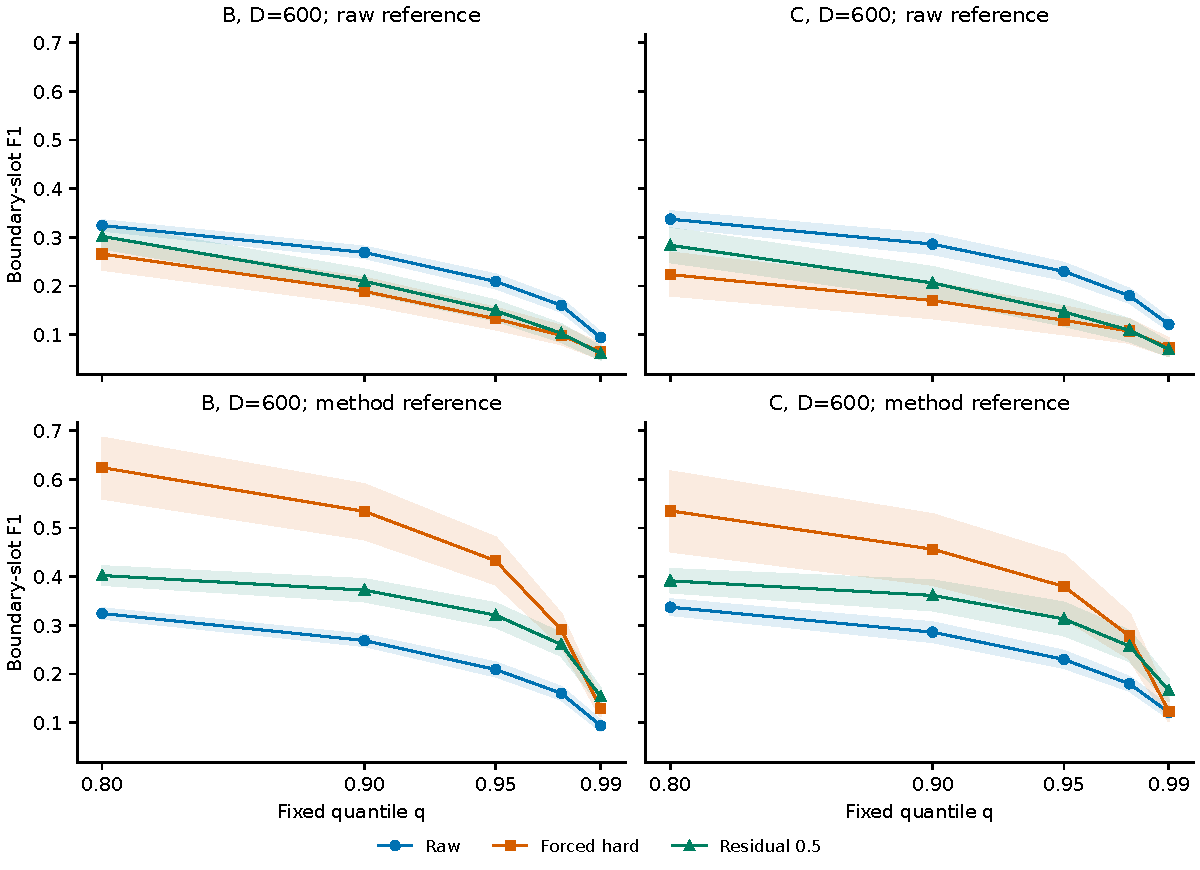
\includegraphics[width=\linewidth]{results/information_sciences/narrative_assets/fig_threshold_curves.pdf}
\caption{Fixed-quantile F1 sensitivity in the B fixed schedule and C central
grid at $D=600$. Rows change the amplitude reference; columns hold inputs
and slot grids fixed. Bands are pointwise $95\%$ repeat-bootstrap intervals,
not simultaneous bands. Every tested quantile is retained, with no best-F1
selection or independent false-alarm calibration.}
\label{fig:threshold-sensitivity}
\end{figure}

\subsection{Within-group and cross-group residual pair credit}
\label{app:residual-pairs}
Let $\mathcal P_e=\{(u,v):A_{u,e}=1,A_{v,e}=0\}$ and
$c(d)=\mathbf1\{d>0\}+\tfrac12\mathbf1\{d=0\}$. For a residual weight
$\lambda$, write
$d^{(\lambda)}_{uv,e}=(1-\lambda)(H_{u,e}-H_{v,e})+
\lambda(S_{u,e}-S_{v,e})$. Partition $\mathcal P_e$ by equality of the
candidate group labels, and define
\begin{equation}
G_g(\lambda)=\frac1{|\mathcal E_\Delta|}\sum_{e\in\mathcal E_\Delta}
\frac{\sum_{(u,v)\in\mathcal P_e^{g}}
 [c(d^{(\lambda)}_{uv,e})-c(d^{(0)}_{uv,e})]}{n_e^+n_e^-},
\quad g\in\{\mathrm{within},\mathrm{cross}\}.
\end{equation}
Each component uses the edge's total positive--negative pair denominator,
then the same macro average as within-edge temporal AUROC. Hence
$G_{\rm within}+G_{\rm cross}=T_{\rm residual}-T_{\rm hard}$ exactly in
the finite score representation, up to reported floating-point differences.
Within a candidate group, $d^{(0)}=0$ and every positive $\lambda$ restores
raw ordering; across groups both nonzero hard contrasts and tied map values
are retained in the accounting. We report all original weights and a fixed
$10^{-8}$ diagnostic weight, together with lost/new ties and reversed
comparisons. A near-zero rank jump is not evidence of robust thresholded
detection or improved latent-state inference.

\begin{table}[!htbp]\centering
\caption{Residual pair-credit accounting on A and the central C grid, Lasso.
Mean within/cross increments sum to residual-minus-hard within-edge temporal AUROC before
rounding. Each edge uses its total positive--negative pair denominator before
macro averaging. The near-zero weight is diagnostic; all fixed weights and
auxiliary conditions remain in the numerical files. At $\lambda=1$, the C
total-contrast interval is the sign-reversed original C forced-minus-raw
interval; within/cross component intervals retain their decomposition stream.}
\label{tab:residual-pairs}
\resizebox{\linewidth}{!}{\begin{tabular}{llrrrrr}
\toprule
Study, $D$ & $\lambda$ & \shortstack{Forced\\hard} & Residual & \shortstack{Within-group\\$\Delta$} & \shortstack{Cross-group\\$\Delta$} & \shortstack{Total\\$\Delta$} \\
\midrule
A, 300 & $10^{-8}$ & 0.639 & 0.707 & \shortstack[r]{$+0.068$\\$[0.059,0.078]$} & \shortstack[r]{$+0.000$\\$[0.000,0.000]$} & \shortstack[r]{$+0.068$\\$[0.059,0.078]$} \\
A, 300 & 0.25 & 0.639 & 0.718 & \shortstack[r]{$+0.068$\\$[0.059,0.078]$} & \shortstack[r]{$+0.011$\\$[0.006,0.016]$} & \shortstack[r]{$+0.079$\\$[0.066,0.092]$} \\
A, 300 & 0.5 & 0.639 & 0.716 & \shortstack[r]{$+0.068$\\$[0.059,0.078]$} & \shortstack[r]{$+0.009$\\$[0.001,0.017]$} & \shortstack[r]{$+0.078$\\$[0.061,0.094]$} \\
A, 300 & 1 & 0.639 & 0.707 & \shortstack[r]{$+0.068$\\$[0.059,0.078]$} & \shortstack[r]{$+0.000$\\$[-0.013,0.013]$} & \shortstack[r]{$+0.069$\\$[0.048,0.090]$} \\
A, 600 & $10^{-8}$ & 0.805 & 0.830 & \shortstack[r]{$+0.025$\\$[0.018,0.032]$} & \shortstack[r]{$+0.000$\\$[0.000,0.000]$} & \shortstack[r]{$+0.025$\\$[0.018,0.032]$} \\
A, 600 & 0.25 & 0.805 & 0.824 & \shortstack[r]{$+0.025$\\$[0.018,0.032]$} & \shortstack[r]{$-0.006$\\$[-0.011,-0.002]$} & \shortstack[r]{$+0.019$\\$[0.009,0.028]$} \\
A, 600 & 0.5 & 0.805 & 0.809 & \shortstack[r]{$+0.025$\\$[0.018,0.032]$} & \shortstack[r]{$-0.021$\\$[-0.027,-0.015]$} & \shortstack[r]{$+0.003$\\$[-0.008,0.015]$} \\
A, 600 & 1 & 0.805 & 0.767 & \shortstack[r]{$+0.025$\\$[0.018,0.032]$} & \shortstack[r]{$-0.063$\\$[-0.072,-0.054]$} & \shortstack[r]{$-0.038$\\$[-0.053,-0.023]$} \\
C, 300 & $10^{-8}$ & 0.661 & 0.740 & \shortstack[r]{$+0.079$\\$[0.066,0.092]$} & \shortstack[r]{$+0.000$\\$[0.000,0.000]$} & \shortstack[r]{$+0.079$\\$[0.066,0.092]$} \\
C, 300 & 0.25 & 0.661 & 0.745 & \shortstack[r]{$+0.079$\\$[0.066,0.092]$} & \shortstack[r]{$+0.005$\\$[-0.007,0.016]$} & \shortstack[r]{$+0.084$\\$[0.062,0.105]$} \\
C, 300 & 0.5 & 0.661 & 0.735 & \shortstack[r]{$+0.079$\\$[0.066,0.092]$} & \shortstack[r]{$-0.005$\\$[-0.024,0.013]$} & \shortstack[r]{$+0.074$\\$[0.044,0.102]$} \\
C, 300 & 1 & 0.661 & 0.707 & \shortstack[r]{$+0.079$\\$[0.066,0.092]$} & \shortstack[r]{$-0.032$\\$[-0.061,-0.005]$} & \shortstack[r]{$+0.047$\\$[0.006,0.084]$} \\
C, 600 & $10^{-8}$ & 0.797 & 0.849 & \shortstack[r]{$+0.052$\\$[0.038,0.067]$} & \shortstack[r]{$+0.000$\\$[0.000,0.000]$} & \shortstack[r]{$+0.052$\\$[0.038,0.067]$} \\
C, 600 & 0.25 & 0.797 & 0.841 & \shortstack[r]{$+0.052$\\$[0.038,0.067]$} & \shortstack[r]{$-0.008$\\$[-0.016,0.001]$} & \shortstack[r]{$+0.044$\\$[0.026,0.063]$} \\
C, 600 & 0.5 & 0.797 & 0.815 & \shortstack[r]{$+0.052$\\$[0.038,0.067]$} & \shortstack[r]{$-0.034$\\$[-0.047,-0.021]$} & \shortstack[r]{$+0.017$\\$[-0.005,0.042]$} \\
C, 600 & 1 & 0.797 & 0.761 & \shortstack[r]{$+0.052$\\$[0.038,0.067]$} & \shortstack[r]{$-0.088$\\$[-0.109,-0.068]$} & \shortstack[r]{$-0.037$\\$[-0.067,-0.002]$} \\
\bottomrule
\end{tabular}
}
\end{table}
\begin{figure}[!htbp]\centering
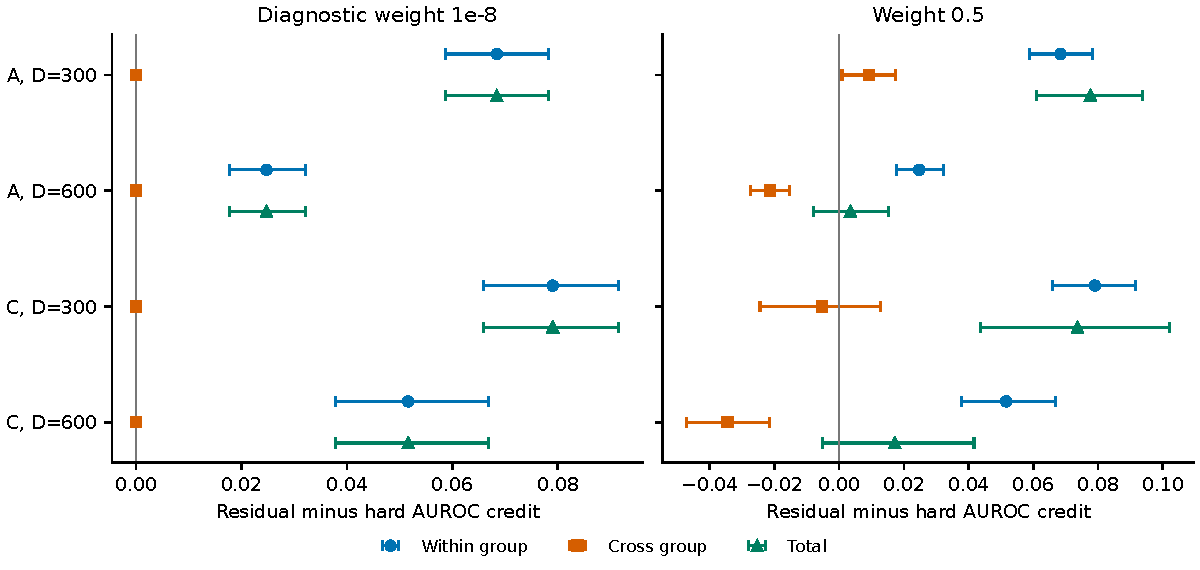
\includegraphics[width=\linewidth]{results/information_sciences/narrative_assets/fig_residual_pairs.pdf}
\caption{Residual within-edge temporal AUROC increments from within-group and cross-group
comparisons. Near-zero residuals break hard-output ties without changing
cross-group credit on these retained arrays. At weight $0.5$, cross-group
reordering can offset that gain. Pointwise intervals use repeat resampling.}
\label{fig:residual-pairs}
\end{figure}

\FloatBarrier
\section{Additional comparisons and exploratory analyses}
\label{supp:additional}

\subsection{Earlier exploratory mechanism grid}
\label{sec:controlled}

\paragraph{Design.}
The earlier exploratory grid has a seven-window reference configuration,
one-factor scans on eight axes, two
interactions, and the control family: 35 configurations with twenty seeds each,
at $N=8$, $L=3$, $h=300$, stride $150$, $T=1200$ unless stated. All fits supply
a state count; the stationary condition is a gate-stress condition with
$K_{\mathrm{candidate}}=2$ and $K_{\mathrm{true}}=1$, and is labelled as such.

\paragraph{Stability of the switching path.}
State tensors whose initial radius exceeds $0.90$ are rescaled as
specified in Section~\ref{app:config}; this does not guarantee stability
of an arbitrary switching path. Across $200$ seeds the
largest absolute value is $0.536$, the largest ratio of that value to the series
standard deviation is $4.97$, the 95th percentile of the per-state variance
ratio is $1.10$, and no trajectory exceeds the blow-up threshold. The largest
recorded per-state companion radius in this audit is $0.6505$, below the
rescaling trigger. The generator is therefore empirically stable on the paths
it is used for, which is weaker
than a joint-stability guarantee.

\paragraph{State duration and purity.}
At state duration $D=150$ ($P{=}300$) every window straddles a boundary
(purity $0.500$), union AUROC is $0.756$ and regime AUPRC $0.465$; at $D=900$
purity is $0.929$, union $0.859$ and regime $0.718$. Lengthening the
\emph{switching} series to $T=3000$ (same $D{=}300$, now $19$ windows) lowers the
measured relative-inertia improvement to $0.090$, below the $0.12$ threshold, so
the gate rejects the two-state partition in $18$ of $20$ fits --- a rejection of
a \emph{true} switch, consistent with the geometric account
(Section~\ref{sec:gate-geometry}) that a fixed threshold has no test meaning
across window counts.

\paragraph{Support retention.}
Union AUROC rises from $0.768$ at configured retention $o=0$ to $0.862$ at $o=1$, and
regime AUPRC from $0.530$ to $0.655$. Measurement noise from $0$ to $0.4$ moves
union AUROC from $0.801$ to $0.777$ and regime AUPRC from $0.587$ to $0.535$;
base-support probability $p$ from $0.10$ to $0.30$ moves union AUROC from $0.786$ to $0.803$
and regime AUPRC from $0.499$ to $0.666$.

\begin{figure}[!htbp]
\centering
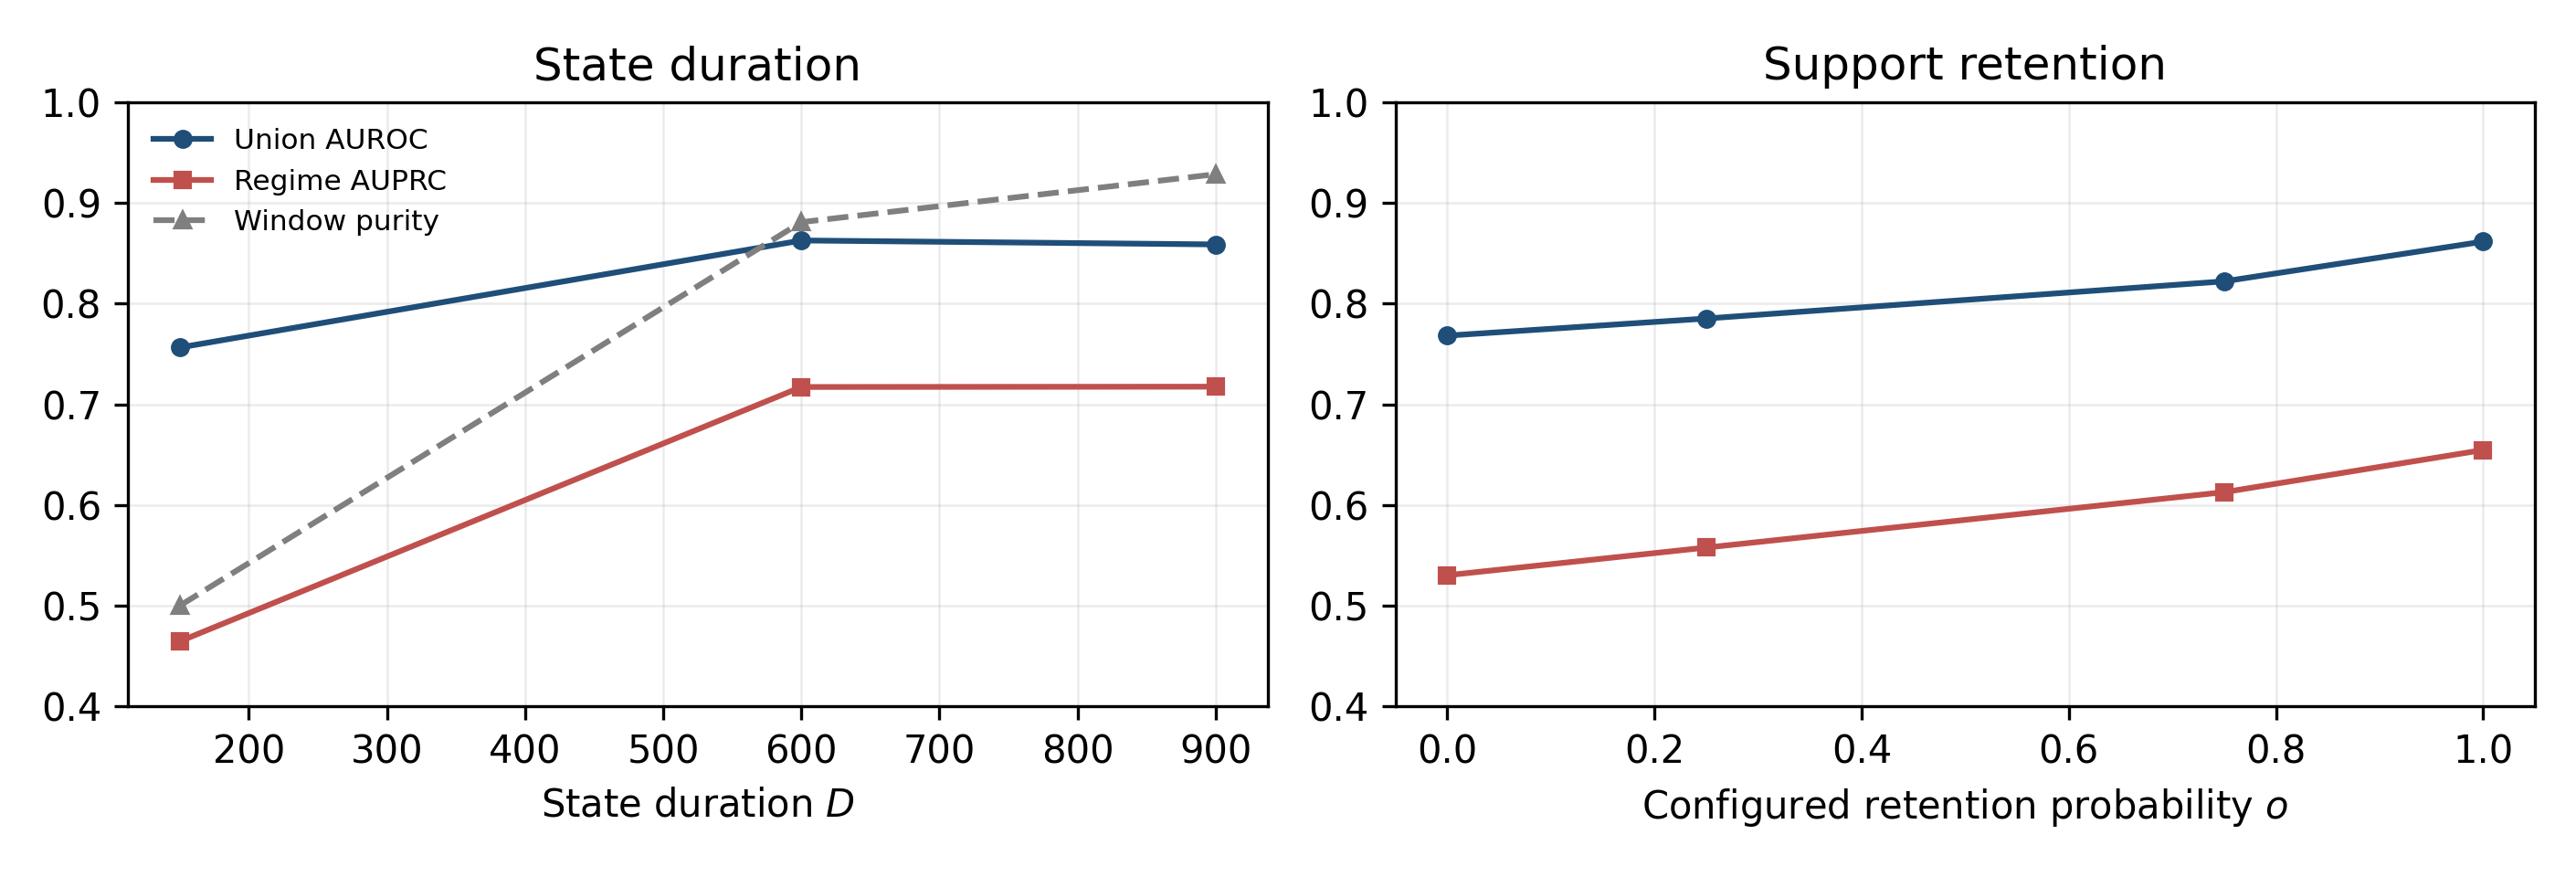
\includegraphics[width=\linewidth]{results/information_sciences/narrative_assets/rev2_mechanism.png}
\caption{Recovery against state duration (left) and configured support retention (right).
The left abscissa is state duration $D$ (the full cycle is $2D$),
and the right abscissa is retention probability $o$, not each draw's realised
overlap. Window purity rises with
duration and tracks both scores.}
\label{fig:mechanism}
\end{figure}

\paragraph{Control taxonomy.}
Table~\ref{tab:controls} groups the controls by what they change and reports the
two structural counts. Three points matter. First, lag shift is a genuine
lag-specific structure change: the pair-level graph is unchanged, so pair AUROC
($0.875$) exceeds lag AUROC ($0.784$), and state ARI ($0.407$) is the highest in
the table. Second, the mechanism family has $\kdyn=2$ but $\kgraph=1$: a sign
flip leaves the absolute coefficients identical and drives regime AUPRC to
$0.462$ with ARI $0.153$, and resampled magnitudes under a shared support leave
ARI at $-0.041$. Because the two states share one binary graph, the regime AUPRC
in these rows scores recovery against a single support and does not test whether
the method distinguished the dynamical states; state-label alignment (ARI) alone
carries that question. Third, the nuisance family also has
$\kdyn=2$ with $\kgraph=1$: mean-only is the worst case for union recovery
($0.640$), while variance-only ($0.881$) and a state-specific trend ($0.672$)
disturb the ranking less, and none of them change the support. The gate accepts
a two-state split in all eight conditions.

\begin{table}[!htbp]
\centering
\caption{Controls grouped by what they change. Only the first block changes the
lag-specific support. $\kdyn$ counts dynamical mechanisms, $\kgraph$ counts
binary supports; Pooled denotes the mixed-ranking, time-indexed AUROC.}
\label{tab:controls}
\resizebox{\linewidth}{!}{\begin{tabular}{llrrrrrrr}
\toprule
Category & Condition & $K_{\mathrm{dyn}}$ & $K_{\mathrm{graph}}$ & Lag AUROC & Pair AUROC & Regime AUPRC & Pooled AUROC & Assignment ARI \\
\midrule
structure change & Switching (reference) & 2 & 2 & 0.801 & 0.792 & 0.587 & 0.776 & +0.292 \\
structure change & Lag shift & 2 & 2 & 0.784 & 0.875 & 0.567 & 0.761 & +0.407 \\
\midrule
mechanism change & Same support & 2 & 1 & 0.847 & 0.824 & 0.634 & 0.810 & -0.041 \\
mechanism change & Sign flip & 2 & 1 & 0.764 & 0.705 & 0.462 & 0.728 & +0.153 \\
\midrule
nuisance change & Variance only & 2 & 1 & 0.881 & 0.861 & 0.701 & 0.839 & -0.096 \\
nuisance change & Mean only & 2 & 1 & 0.640 & 0.604 & 0.373 & 0.649 & -0.143 \\
nuisance change & Trend & 2 & 1 & 0.672 & 0.628 & 0.402 & 0.660 & -0.148 \\
\midrule
no change & Stationary & 1 & 1 & 0.908 & 0.883 & 0.775 & 0.871 & +0.000 \\
\bottomrule
\end{tabular}
}
\end{table}

\begin{figure}[!htbp]
\centering
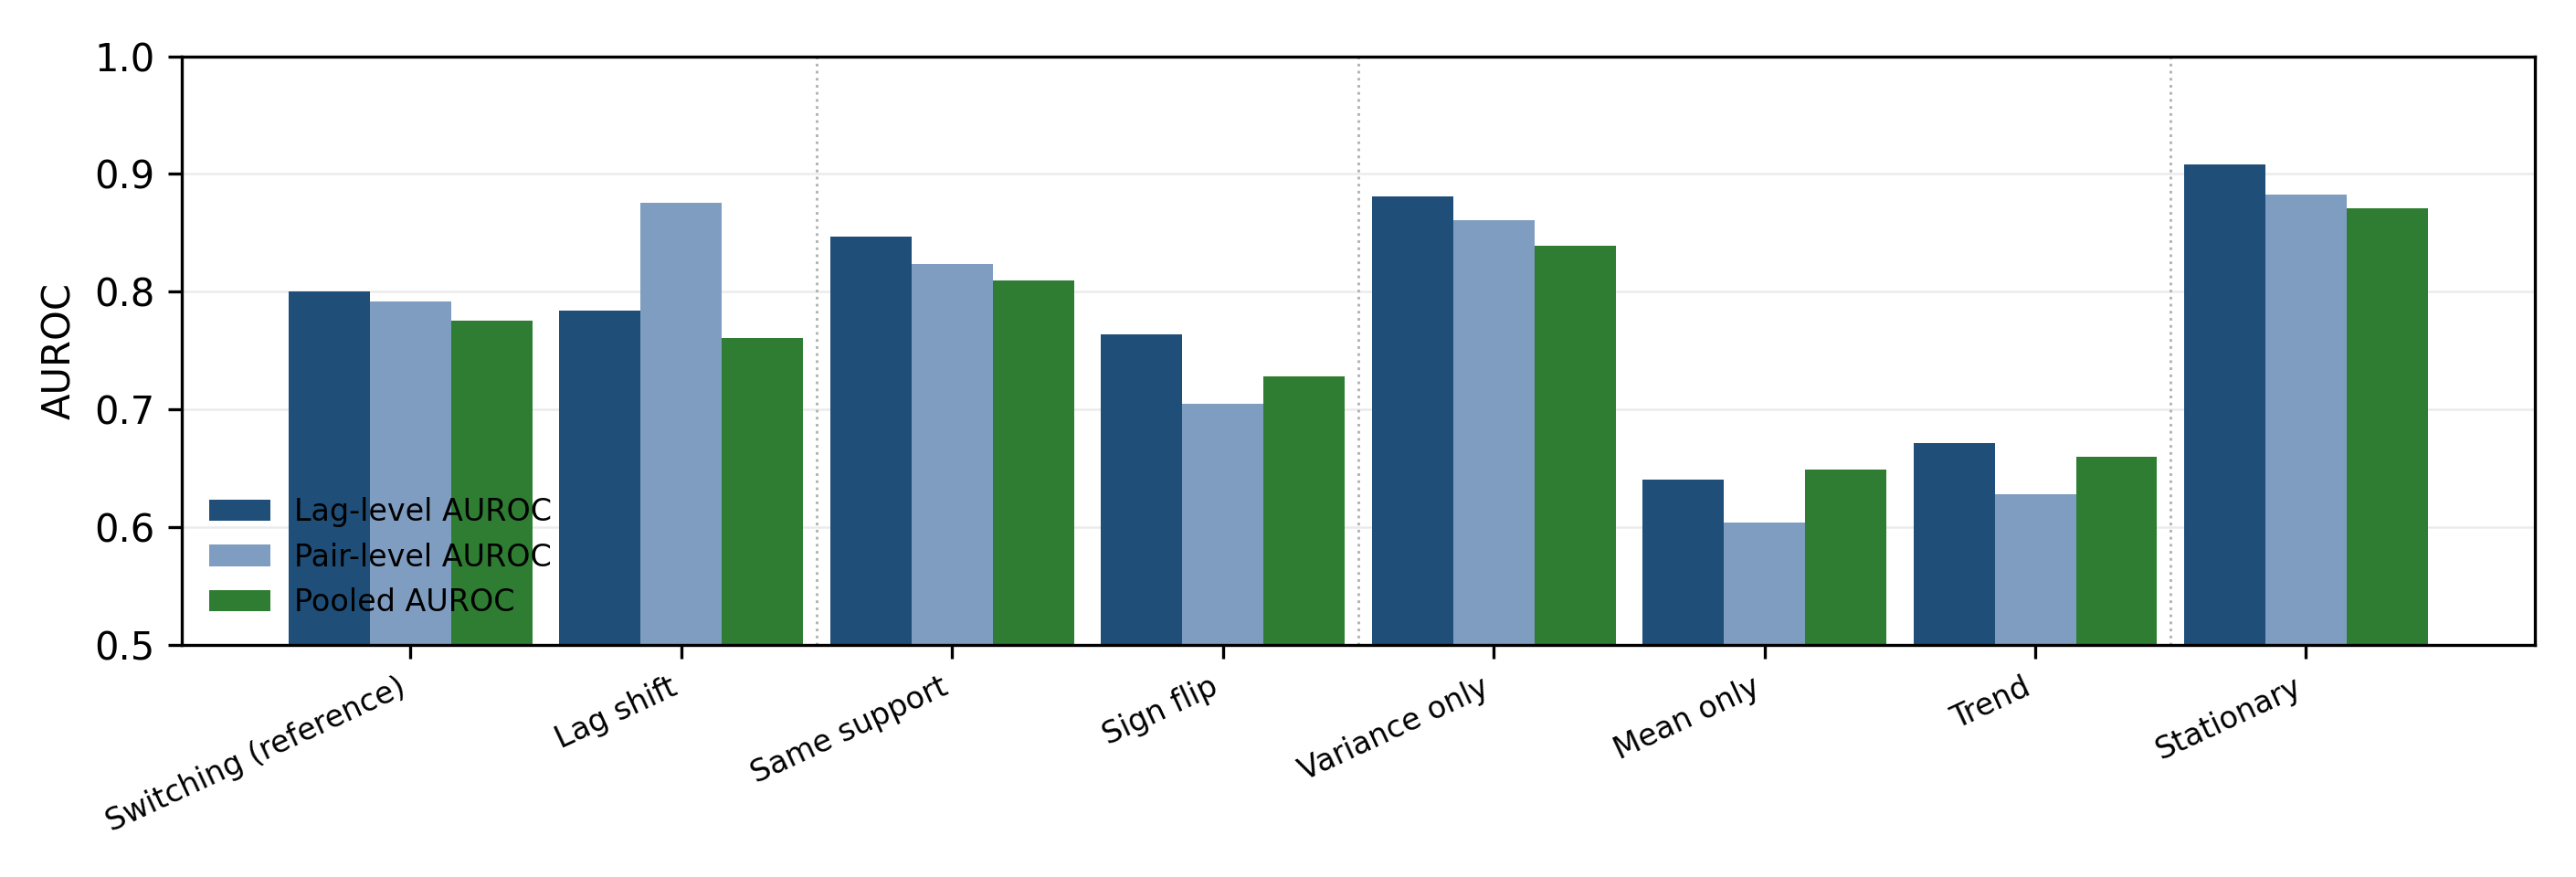
\includegraphics[width=\linewidth]{results/information_sciences/narrative_assets/rev2_controls.png}
\caption{Lag-level, pair-level and pooled AUROC by control family. The
lag-shift condition is easier at the pair level and harder at the lag level, and
it has the highest state ARI: it is a real lag-specific change.}
\label{fig:controls}
\end{figure}

\subsection{Earlier aggregation comparisons across targets}
\label{sec:aggregation}

Every method in this section consumes the same window-level Lasso scores; only
the grouping and aggregation rule changes. Table~\ref{tab:aggregation} reports
union, regime and pooled AUROC on the same scale.

On the switching setting, window mean reaches $0.804$ union AUROC, window max
$0.804$, bagging $0.800$, random balanced grouping $0.798$, K-means $0.801$,
GMM responsibility-weighted maps with argmax emission $0.789$, and temporal DP
$0.795$; the spread is $0.015$.
Regime AUROC stays in the same narrow band ($0.786$ K-means, $0.783$ random,
$0.805$ oracle labels, $0.777$ soft). The pooled AUROC is lower
overall, but the static predictors -- which emit the same graph at every window
-- reach $0.795$ (window mean), $0.791$ (window maximum) and $0.792$ (bagging),
already above fitted K-means ($0.776$), random grouping ($0.773$) and temporal
DP ($0.765$); only oracle labels ($0.806$) improve on a constant graph.

Table~\ref{tab:temporal-delta} shows this pooled reading is incomplete. The
within-edge temporal AUROC $\mathrm{T\!-\!AUC}_{\Delta}$ isolates
within-edge temporal discrimination from long-run occupancy: K-means scores
$0.649$ (bootstrap $95\%$ CI $[0.594,0.705]$), above the
$0.5$ of every constant prediction and the $0.570$ of random grouping, while
oracle labels reach $0.814$ and temporal DP $0.562$. The raw window scores,
used with no grouping, reach $0.716$ (CI $[0.694,0.738]$) --- \emph{above}
K-means. The within-edge temporal discrimination signal therefore
already lives in the local scores, and at this core setting state aggregation compresses it rather
than creating it, even as it improves the pooled metric ($0.776$ vs $0.731$). On
the pooled target the fitted clustering does not beat the static controls, but on
the changing-edge target it beats the constant prediction and the random grouping
while trailing both the raw window scores and the oracle reference: the two
targets measure different abilities, and neither alone reports both.

\begin{table}[!htbp]
\centering
\caption{Aggregation controls on the switching and stationary settings (twenty
seeds). All rows share the same window scores. The GMM row weights state maps
softly but uses argmax responsibility for emission. U is union, R is regime-specific,
and Pooled is the mixed-ranking, time-indexed AUROC; ``--'' marks methods without state scores.}
\label{tab:aggregation}
\resizebox{\linewidth}{!}{\begin{tabular}{lrrrrrr}
\toprule
& \multicolumn{3}{c}{Switching} & \multicolumn{3}{c}{Stationary} \\
\cmidrule(lr){2-4}\cmidrule(lr){5-7}
Method & U-AUROC & R-AUROC & Pooled AUROC & U-AUROC & R-AUROC & Pooled AUROC \\
\midrule
Window mean & 0.804 & -- & 0.795 & 0.919 & -- & 0.919 \\
Window max & 0.804 & -- & 0.791 & 0.893 & -- & 0.893 \\
Bagged mean & 0.800 & -- & 0.792 & 0.918 & -- & 0.918 \\
Random balanced & 0.798 & 0.783 & 0.773 & 0.910 & 0.893 & 0.887 \\
Gated hard & 0.801 & 0.786 & 0.776 & 0.908 & 0.886 & 0.871 \\
GMM weighted + argmax & 0.789 & 0.777 & 0.776 & 0.906 & 0.896 & 0.876 \\
Temporal DP & 0.795 & 0.775 & 0.765 & 0.909 & 0.889 & 0.873 \\
Oracle label & 0.814 & 0.805 & 0.806 & 0.919 & 0.919 & 0.919 \\
Oracle refit & 0.844 & -- & -- & 0.954 & -- & -- \\
\bottomrule
\end{tabular}
}
\end{table}

\begin{table}[!htbp]
\centering
\caption{Pooled AUROC against the within-edge temporal AUROC
$\mathrm{T\!-\!AUC}_{\Delta}$ on the switching setting (twenty seeds; each
sequence has $27.3$ changing edges on average). ``Raw window'' emits each
window's own scores with no grouping. Constant predictions score $0.5$ on the
changing-edge metric by construction; the static ceiling
(Eq.~\ref{eq:static-ceiling}) is $0.979$. The K-means advantage over random
grouping on $\mathrm{T\!-\!AUC}_{\Delta}$ is $p{=}0.016$ (two-sided paired
$t$-test, unadjusted, $n{=}20$, difference $0.080$, $95\%$ CI
$[0.023,0.138]$). The raw-window advantage over K-means is $0.067$ (two-sided
paired $t$-test, unadjusted, $p{=}0.03$, $95\%$ CI $[0.013,0.123]$), replicated
on an untouched seed block ($0.053$, $95\%$ CI $[0.025,0.081]$, $n{=}50$).}
\label{tab:temporal-delta}
\begin{tabular}{lcc}
\toprule
Method & Pooled AUROC & Within-edge AUROC \\
\midrule
Window mean & 0.795 & 0.500 \\
Window max & 0.791 & 0.500 \\
Bagged mean & 0.792 & 0.500 \\
Raw window (no grouping) & 0.731 & 0.716 \\
Random balanced & 0.773 & 0.570 \\
Gated hard & 0.776 & 0.649 \\
GMM weighted + argmax & 0.776 & 0.608 \\
GMM continuous soft & 0.776 & 0.608 \\
Temporal DP & 0.765 & 0.562 \\
Oracle label & 0.806 & 0.814 \\
\midrule
Static ceiling $\mathrm{AUC}^*_{\mathrm{static}}$ & \multicolumn{2}{c}{0.979} \\
\bottomrule
\end{tabular}

\end{table}

\begin{figure}[!htbp]
\centering
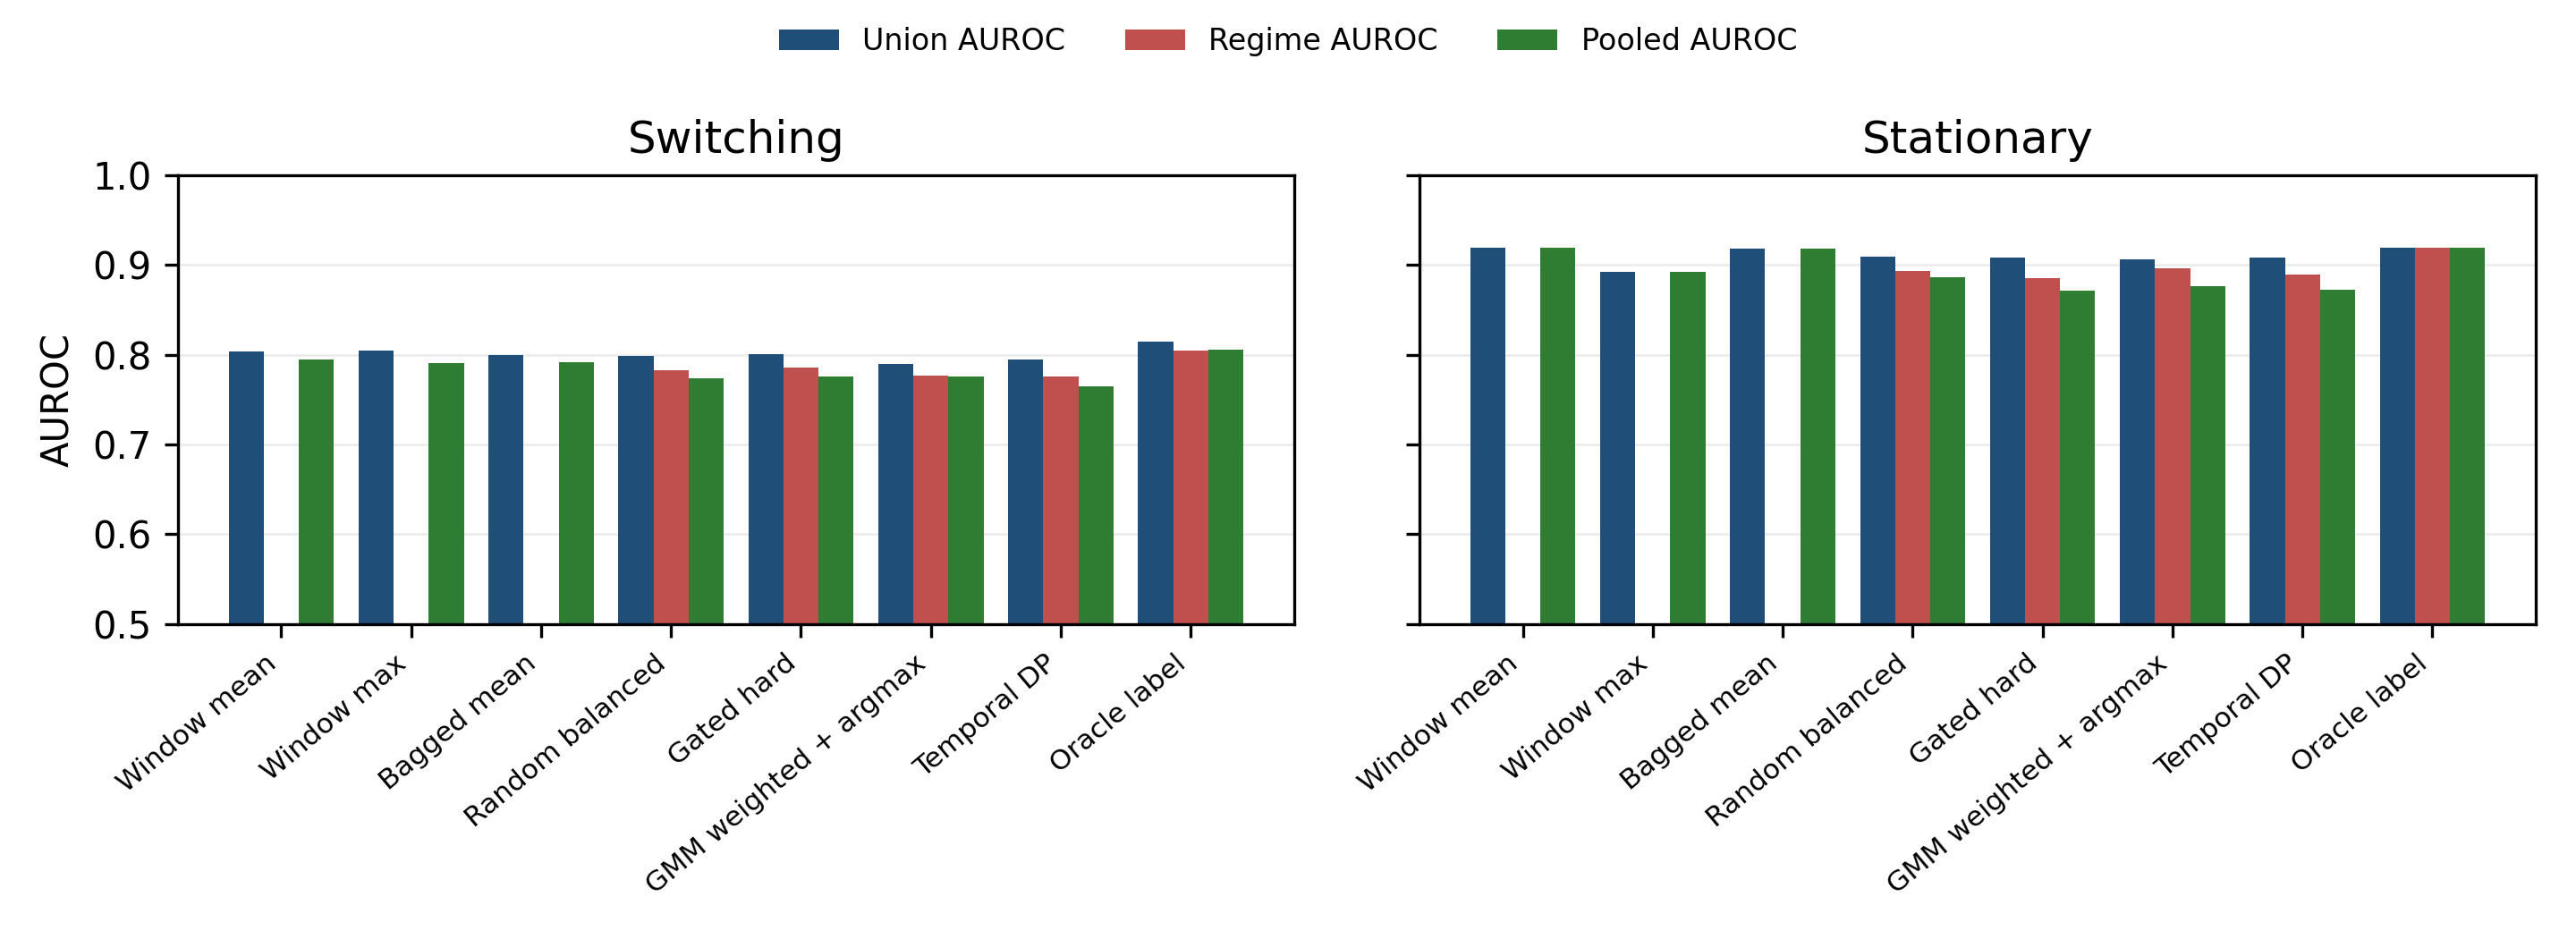
\includegraphics[width=\linewidth]{results/information_sciences/narrative_assets/rev2_aggregation.png}
\caption{Union, regime and pooled AUROC for identical window scores.
Union and regime are flat across aggregation rules; on the pooled target the
static predictors and fitted clustering are close, and only the oracle
assignment improves it.}
\label{fig:aggregation}
\end{figure}

\paragraph{Precision--recall and prevalence.}
Table~\ref{tab:layers} reports the two layers with prevalence, AUPRC lift, and
normalized AP. With prevalence $0.249$ for union edges and $0.174$ for regime edges, the lift
says the regime layer is easier ($3.38\times$ against $2.79\times$); normalized
AP says it is harder ($0.500$ against $0.593$). Both
are correct, and they differ because lift has an upper bound of $1/\pi$ that
grows as prevalence falls. We therefore do not claim an ordering: under the
evaluated generator and protocol, union and regime AUROC are close, while their
precision--recall behaviour differs with prevalence and with the choice of
normalization.

\begin{table}[!htbp]
\centering
\caption{The two layers on the switching setting. Lift and normalized AP
disagree about which layer is easier; we report both and draw no ordering.}
\label{tab:layers}
\begin{tabular}{lrrrrr}
\toprule
Layer & Prevalence & AUROC & AUPRC & AUPRC / prev. & Normalized AP \\
\midrule
Union & 0.249 & 0.801 & 0.694 & 2.79$\times$ & 0.593 \\
Regime-specific & 0.174 & 0.786 & 0.587 & 3.38$\times$ & 0.500 \\
\bottomrule
\end{tabular}

\end{table}

\paragraph{Label error.}
Figure~\ref{fig:eta} sweeps symmetric label error on the K-means partition and,
separately, on the true labels. Under K-means corruption union AUROC moves from
$0.801$ to $0.798$, regime AUPRC from $0.587$ to $0.568$, and ARI from $0.292$
to $-0.041$, while the pooled AUROC is almost flat ($0.776$ to $0.775$)
because the two fitted state scores are already similar. Under oracle corruption
union AUROC moves from $0.814$ to $0.794$, regime AUPRC from $0.639$ to $0.556$,
and the pooled AUROC from $0.806$ to $0.775$. In this configuration, pooled
AUROC changes more under corruption of the true labels than of the fitted
partition.

\begin{figure}[!htbp]
\centering
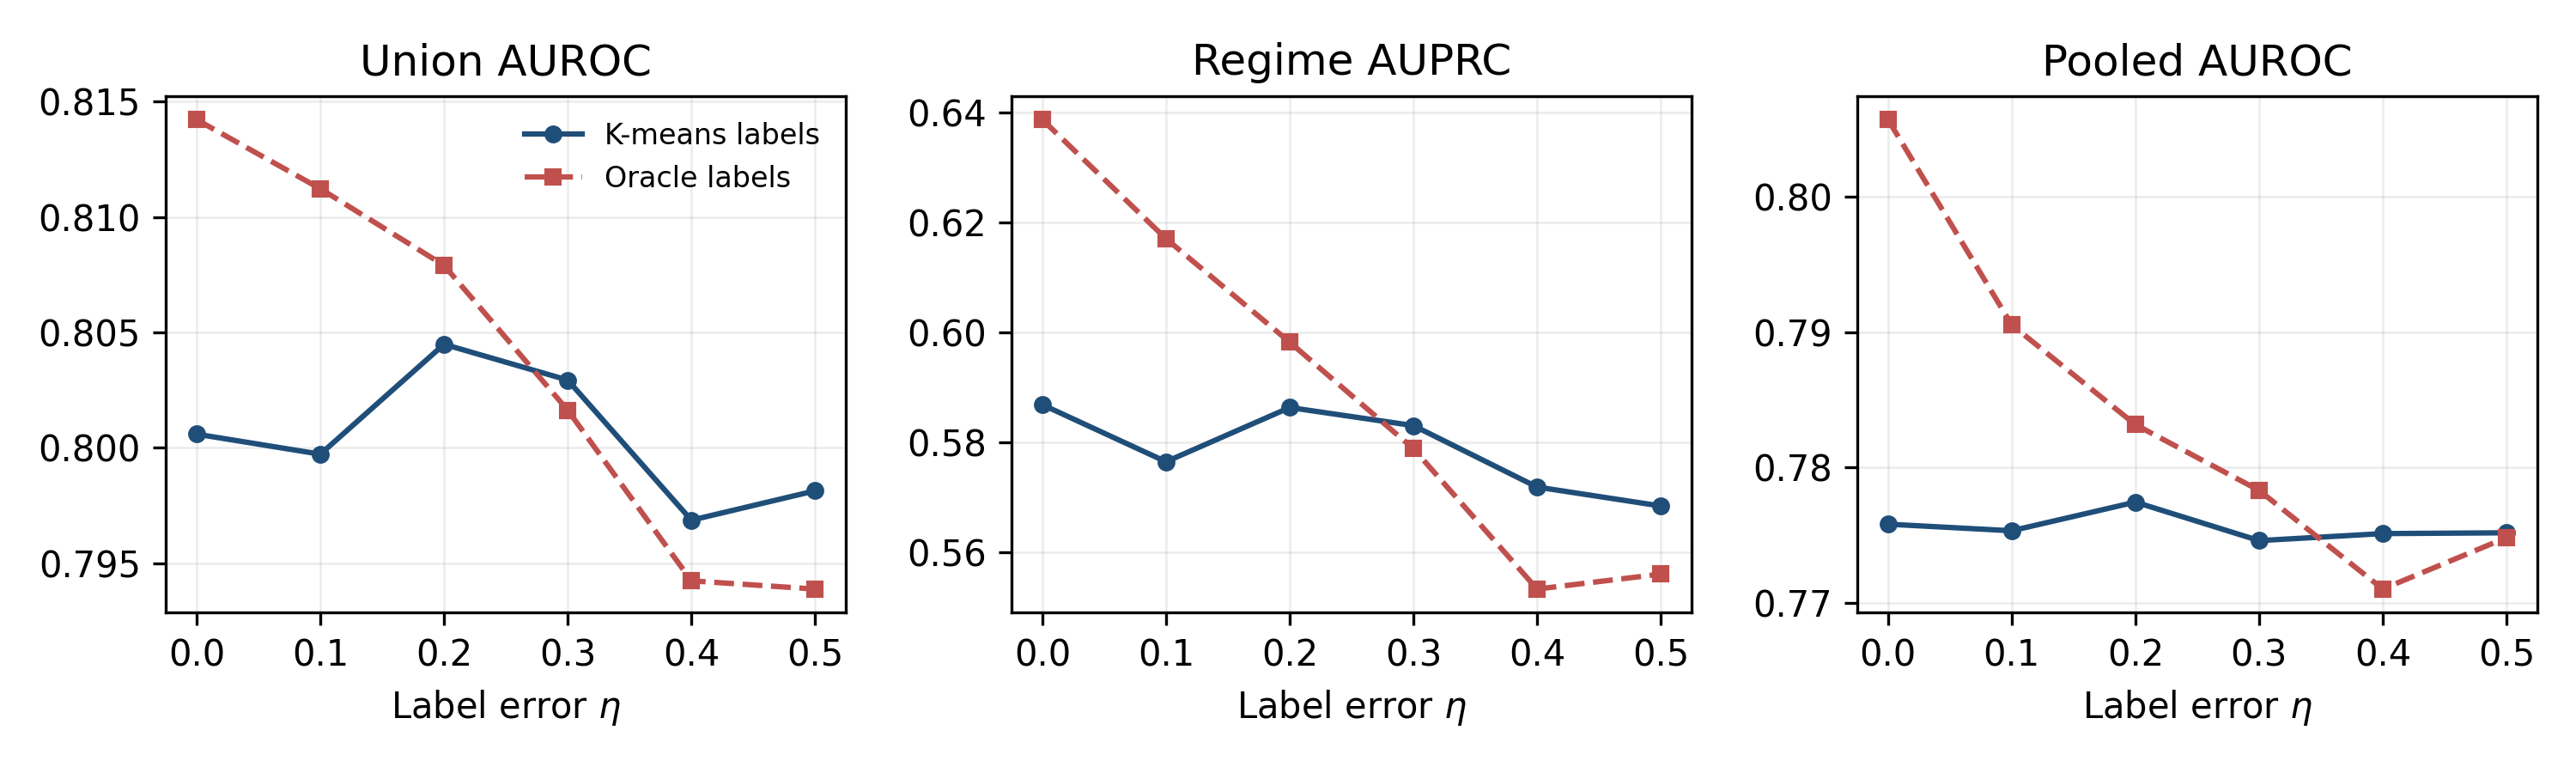
\includegraphics[width=\linewidth]{results/information_sciences/narrative_assets/rev2_eta.png}
\caption{Sensitivity to label corruption applied to the fitted partition
(solid) and the true labels (dashed). Union, regime-specific and pooled recovery
respond differently to label corruption. Changes in pooled AUROC alone do not
identify changes in within-edge temporal discrimination.}
\label{fig:eta}
\end{figure}

\subsection{Exploratory duration and record-length scans}
\label{sec:temporal-grid}

We re-evaluate all $35$ labelled entries of the existing mechanism grid at seeds
$0$--$19$, reusing the four repeated configurations: $31$ distinct configurations
give $620$ configuration--seed fits. This is an exploratory extension on existing
simulation seeds. Each method consumes the same local scores, and the paired
quantity is
\begin{equation}
\Delta_{\mathrm{temporal}}
=\mathrm{T\!-\!AUC}_{\Delta,\mathrm{aggregation}}
-\mathrm{T\!-\!AUC}_{\Delta,\mathrm{raw}}.
\label{eq:temporal-gain}
\end{equation}
Table~\ref{tab:temporal-grid} and Figure~\ref{fig:temporal-grid} show the existing
one-factor duration and length scans. In the former $h=300$, $T=1200$ and $M=7$
are fixed while $D$ varies; in the latter $h=D=300$ and stride $150$ are fixed
while $T=600,1200,3000$ gives $M=3,7,19$. Thus $M$ changes together with record
length and number of switches; these are not independent interventions on $M$
or a crossed $h/D$-by-$M$ grid. Intervals are pointwise $95\%$ percentile
bootstrap intervals of paired seed differences ($10{,}000$ resamples), with no
simultaneous-coverage or confirmatory significance claim. Undefined changing-edge
targets are retained as missing, with evaluable denominators in the full CSV.

\paragraph{Duration changes the sign of the observed gain.}
The hard gate accepts $20/20$ fits at every duration level. At $h/D=1/2$,
raw and hard within-edge temporal AUROC are $0.767$ and $0.798$, a paired gain of $+0.031$
with interval $[0.005,0.057]$. At $h/D=1/3$ the gain is $+0.017$
$[-0.013,0.043]$; at $h/D=1$ it is $-0.067$ $[-0.123,-0.013]$.
At the full-cycle window $h/D=2$, raw is already near chance ($0.517$) and
hard aggregation changes it by $-0.012$ $[-0.021,-0.003]$. The small loss there
does not represent good within-edge temporal discrimination. Oracle labels have positive mean
gains across these levels, but at $h/D=2$ their $+0.029$ interval
$[-0.009,0.064]$ includes zero. The earlier exploratory reference configuration's loss therefore does
not extend uniformly across durations.

\paragraph{Matched random grouping at the selected positive cell.}
At $D=600$, we enumerate every two-group partition with the fitted group sizes
for each seed: $21$ or $35$ unlabelled partitions, $616$ in total. Each partition
rebuilds its own within-group means and is scored before its AUROC is averaged
within the seed. The twenty simulation seeds, not the enumerated partitions,
are the statistical units. The matched-random mean is $0.577$, versus hard
$0.798$ and raw $0.767$. Hard exceeds matched random by $+0.222$
$[0.193,0.250]$, while matched random is below raw by $-0.191$
$[-0.204,-0.179]$ (Table~\ref{tab:matched-grouping}). Thus hard's positive
comparison with raw is accompanied by added value over this size-matched random
control. It is not explained by arbitrary grouping-and-averaging under that
control, but remains an exploratory result at a selected cell on existing seeds.

\paragraph{Connecting conditional gains to the two-state identity.}
Table~\ref{tab:grouping-factors} reports three hard-candidate
conditions. Extending $D$ from $300$ to $600$ at fixed $h=300,M=7$ raises both
mean state-assignment discrimination and mean contrast concordance; the mean product
increases from $0.298$ to $0.596$, recovering the hard AUROCs through
Eq.~\eqref{eq:state-factor}. The forced $M=19$ candidate has core-like state-assignment
discrimination, a higher contrast concordance and mean product $0.359$, giving
hard AUROC $0.679$ against raw $0.722$. These profiles connect the conditions
to the same identity without assigning independent causal roles to the two
jointly estimated factors. The factors' marginal means are never multiplied
to reconstruct a mean AUROC.

\paragraph{Gate fallback and executed aggregation answer different questions.}
For $M=3,7,19$, gated hard gains are $-0.017$, $-0.067$ and $-0.202$;
acceptance is $20/20$, $20/20$ and $2/20$. At $M=19$, forcing the same hard
candidate on all seeds gives $-0.042$ $[-0.089,0.006]$, whereas the gated
pipeline gives $-0.202$ $[-0.229,-0.164]$. The $18$ rejected fits emit a
constant window-maximum graph with within-edge temporal AUROC $0.5$; fallback therefore
adds $-0.160$ to the all-seed mean difference relative to the forced candidates.
Among the two fits that actually aggregate, hard gain is $-0.046$ against their
own raw baseline ($0.742$). This selected subgroup is too small for an interval
under our rule of at least five evaluable seeds. Section~\ref{app:temporal-grid}
reports accepted-subgroup contrasts for all methods on the same seeds, as well
as gated hard execution counts. GMM and oracle have no acceptance gate and aggregate
in all $20$ fits per displayed cell; the shared hard-gate subgroup does not
introduce a gate for either comparator.

\paragraph{The tested GMM does not provide a diffuse soft control.}
We distinguish responsibility-weighted state maps with argmax
emission from continuous emission
$\widehat S_w=\sum_k r_{wk}\widehat G_k$, where
$\widehat G_k=\sum_v r_{vk}S_v/\sum_v r_{vk}$. Both use the same two-component
diagonal GMM, three initialisations and simulation seed. Table~\ref{tab:temporal-delta}
includes both: at the core point they each reach $0.608$, giving continuous
soft gain $-0.109$ $[-0.156,-0.060]$. Continuous soft mean gains are negative
at all six distinct displayed configurations. All $620$ GMM fits converge, but
no window has maximum responsibility below $0.99$; the largest mean normalised
responsibility entropy is only $2.15\times10^{-7}$. Thus this fitted model is
nearly a hard assignment and does not isolate the benefit of diffuse memberships.
A post-run $12$-decimal score-rounding check preserves this conclusion; it removes
some tiny continuous/argmax ranking differences (Section~\ref{app:temporal-grid}).
These results do not establish that soft aggregation generally fails.

\begin{table}[!htbp]
\centering
\caption{Paired temporal gain over raw windows on the existing duration and length
scans (twenty seeds per cell). Raw is absolute within-edge temporal AUROC; all other score
columns are $\Delta_{\mathrm{temporal}}$. Gate counts concern gated hard.
Forced hard bypasses only that gate. GMM uses continuous responsibility emission;
oracle averages by true window labels, without refitting. The reference cell
appears once in each scan and is not an independent replication.}
\label{tab:temporal-grid}
\resizebox{\linewidth}{!}{\begin{tabular}{lrrrrrrr}
\toprule
Scan/level & $M$ & Gate & Raw & Gated $\Delta$ & Forced hard $\Delta$ & GMM soft $\Delta$ & Oracle $\Delta$ \\
\midrule
\multicolumn{8}{l}{Duration scan ($M=7$)} \\
$h/D=1/3$ & 7 & 20/20 & 0.792 & +0.017 & +0.017 & -0.046 & +0.060 \\
$h/D=1/2$ & 7 & 20/20 & 0.767 & +0.031 & +0.031 & -0.061 & +0.071 \\
$h/D=1$ & 7 & 20/20 & 0.716 & -0.067 & -0.067 & -0.109 & +0.097 \\
$h/D=2$ & 7 & 20/20 & 0.517 & -0.012 & -0.012 & -0.019 & +0.029 \\
\midrule
\multicolumn{8}{l}{Length scan ($h/D=1$)} \\
$M=3$ & 3 & 20/20 & 0.684 & -0.017 & -0.017 & -0.030 & +0.004 \\
$M=7$ & 7 & 20/20 & 0.716 & -0.067 & -0.067 & -0.109 & +0.097 \\
$M=19$ & 19 & 2/20 & 0.722 & -0.202 & -0.042 & -0.102 & +0.160 \\
\bottomrule
\end{tabular}
}
\end{table}

\begin{table}[!htbp]
\centering
\caption{Three-condition two-state diagnostics, twenty seeds each at $h=300$.
Hard and Raw are within-edge temporal AUROCs. The identity uses the mean
per-seed product, not the product of marginal means. The $M=19$ row bypasses
the gate and evaluates the unchanged hard candidate on all seeds. Factors are
aligned by the same truth-overlap label matching used in the core diagnostic.}
\label{tab:grouping-factors}
\resizebox{\linewidth}{!}{\begin{tabular}{rrlrrrrr}
\toprule
$D$ & $M$ & Hard output & $\mathbb E[J]$ & $\mathbb E[C_{\rm edge}]$ & $\mathbb E[JC_{\rm edge}]$ & Hard & Raw \\
\midrule
300 & 7 & Gated & 0.533 & 0.414 & 0.298 & 0.649 & 0.716 \\
600 & 7 & Gated & 0.867 & 0.686 & 0.596 & 0.798 & 0.767 \\
300 & 19 & Forced & 0.537 & 0.581 & 0.359 & 0.679 & 0.722 \\
\bottomrule
\end{tabular}
}
\end{table}

For the same seeds, writing $T$ for within-edge temporal AUROC, the existing
two-state identity gives
\begin{equation}
\overline{\Delta}_{\mathrm{temporal}}
=\overline{T}_{\mathrm{hard}}-\overline{T}_{\mathrm{raw}}
=\frac12\left[\overline{JC_{\mathrm{edge}}}
-\left(2\overline{T}_{\mathrm{raw}}-1\right)\right].
\label{eq:temporal-gain-factor}
\end{equation}
Hard aggregation improves on raw when its joint grouping--contrast ability
$\overline{JC_{\mathrm{edge}}}$ exceeds the temporal ability already present
in raw scores, $2\overline{T}_{\mathrm{raw}}-1$.
From $D=300$ to $600$ at $M=7$, hard gains $0.149$ while raw gains $0.051$,
so hard-minus-raw improves by $0.098$; this is a descriptive rewriting of the
existing results, not a new theorem or a general rule for choosing $D$.

\begin{figure}[!htbp]
\centering
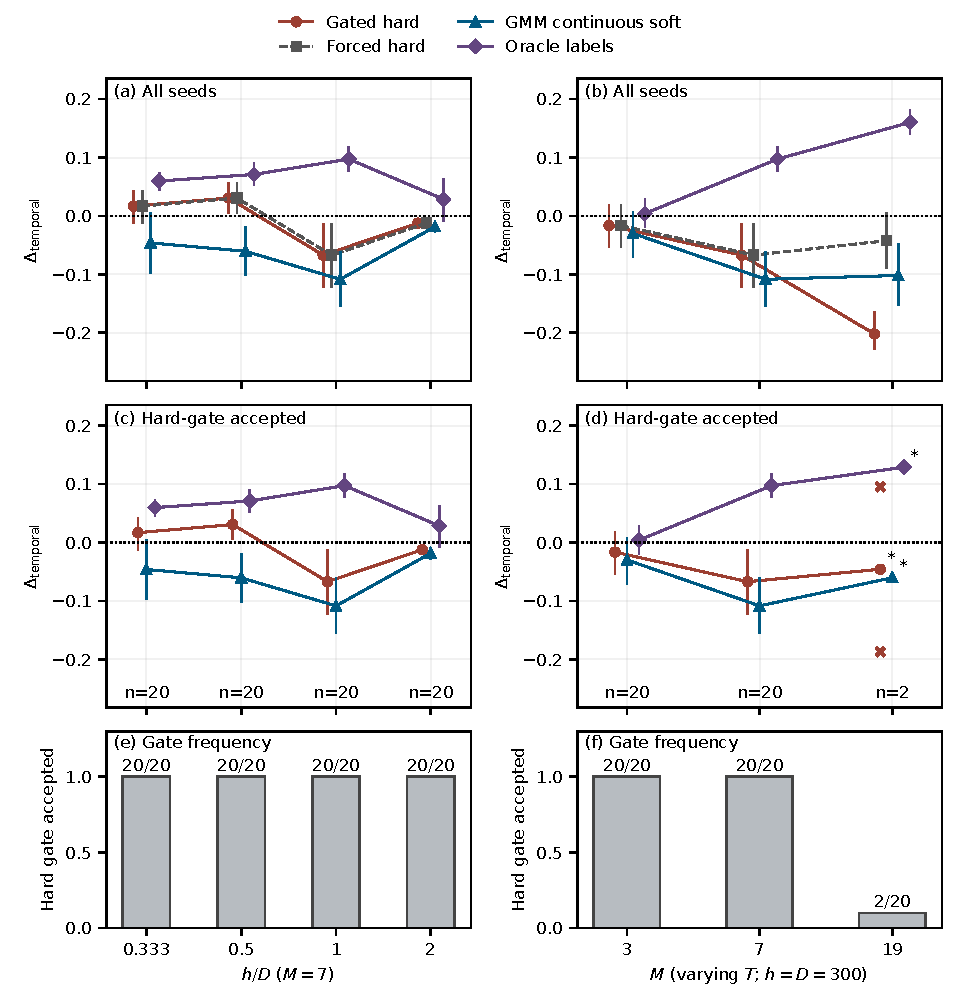
\includegraphics[width=0.98\linewidth]{results/information_sciences/narrative_assets/rev2_temporal_grid.pdf}
\caption{Temporal gain and gate selection at discrete existing grid levels.
(a,b) All-seed paired gains and pointwise $95\%$ bootstrap intervals; zero is
the raw-window reference. (c,d) The same comparison on the common hard-gate
accepted seeds; forced hard coincides with gated hard there and is omitted.
Asterisks mean fewer than five seeds, so no interval is shown; crosses show
the two individual hard gains at $M=19$. These selected-subgroup means are
descriptive. (e,f) Hard-gate acceptance; GMM and oracle execute without this
gate in all twenty fits per cell. Left: vary $D$ at fixed $M=7$. Right: vary
$T$ to change $M$ at fixed $h=D=300$.}
\label{fig:temporal-grid}
\end{figure}

\subsection{Matched partitions, gate subgroups, and GMM sensitivity}
\label{app:temporal-grid}

\paragraph{Exact matched grouping control.}
The selected positive cell has $D=600,h=300,T=1200,M=7$. For each fitted
partition, use the smaller group size $k$ and enumerate all $\binom7k$ memberships,
with complement labels representing the same unlabelled partition. Observed
sizes give $21$ or $35$ partitions per seed. Each partition estimates its own
maps, emits them using its own assignments and yields one within-edge temporal AUROC.
Average these AUROCs within seed before computing the twenty paired contrasts.
Averaging prediction tensors first would be a different estimator and is not
used. The corresponding partition rows and within-seed summaries are retained
in the supplementary archive; the three contrasts are exploratory and their
intervals are pointwise rather than a new confirmatory family.

\begin{table}[!htbp]
\centering
\caption{Selected-cell exact group-size-matched random control. Intervals resample
the twenty seeds, after averaging partition AUROCs within each seed. The $616$
partitions are not independent replications.}
\label{tab:matched-grouping}
\begin{tabular}{lrrr}
\toprule
Comparison & Mean difference & Pointwise 95\% CI & Seeds \\
\midrule
Gated hard $-$ raw & +0.031 & [+0.005, +0.057] & 20 \\
Gated hard $-$ matched random & +0.222 & [+0.193, +0.250] & 20 \\
Matched random $-$ raw & -0.191 & [-0.204, -0.179] & 20 \\
\bottomrule
\end{tabular}

\end{table}

The full grid contributes $35\times20\times5=3{,}500$ method rows, including the
GMM argmax variant. Four duplicate configurations reuse their original
observations, giving $620$ distinct configuration--seed fits. For $240$ of the
$700$ labelled configuration--seed contexts, no changing edge flips in the
evaluation windows (including support-preserving controls and the rare-state
condition); their within-edge temporal AUROC and gains remain undefined, rather than $0.5$.
Table~\ref{tab:temporal-coverage} gives the evaluable counts and missing-target
reasons for every labelled configuration. Repeated configuration IDs reuse
the same observations rather than contributing independent data.

The summary CSV includes all-seed, common hard-gate accepted/rejected, and each
method's actual execution subset. Table~\ref{tab:temporal-grid-accepted} shows the
common accepted subset so each contrast retains its own paired raw baseline.
For gated hard it is exactly the execution subset; forced hard is
evaluated on all seeds. Ungated GMM and oracle also execute on all seeds.
At $M=19$, selection leaves two hard
gains of opposite signs, so neither the accepted-only mean nor the all-seed
forced mean supports a precise general conclusion about long-record aggregation.

\begin{table}[!htbp]
\centering
\caption{Paired gains on the common hard-gate accepted subset. $n$ is the number
of evaluable accepted seeds; Raw is their own absolute within-edge temporal AUROC. Intervals
are pointwise paired-seed bootstrap intervals; [--] means fewer than five seeds,
not a missing mean. GMM and oracle remain ungated comparators.}
\label{tab:temporal-grid-accepted}
\resizebox{\linewidth}{!}{\begin{tabular}{lrrrrr}
\toprule
Scan/level & $n$ & Raw & Gated $\Delta$ [95\% CI] & GMM soft $\Delta$ [95\% CI] & Oracle $\Delta$ [95\% CI] \\
\midrule
\multicolumn{6}{l}{Duration scan ($M=7$)} \\
$h/D=1/3$ & 20 & 0.792 & +0.017 [-0.013, +0.043] & -0.046 [-0.099, +0.005] & +0.060 [+0.044, +0.074] \\
$h/D=1/2$ & 20 & 0.767 & +0.031 [+0.005, +0.057] & -0.061 [-0.102, -0.018] & +0.071 [+0.052, +0.092] \\
$h/D=1$ & 20 & 0.716 & -0.067 [-0.123, -0.013] & -0.109 [-0.156, -0.060] & +0.097 [+0.077, +0.118] \\
$h/D=2$ & 20 & 0.517 & -0.012 [-0.021, -0.003] & -0.019 [-0.028, -0.009] & +0.029 [-0.009, +0.064] \\
\midrule
\multicolumn{6}{l}{Length scan ($h/D=1$)} \\
$M=3$ & 20 & 0.684 & -0.017 [-0.055, +0.019] & -0.030 [-0.071, +0.008] & +0.004 [-0.020, +0.030] \\
$M=7$ & 20 & 0.716 & -0.067 [-0.123, -0.013] & -0.109 [-0.156, -0.060] & +0.097 [+0.077, +0.118] \\
$M=19$ & 2 & 0.742 & -0.046 [--] & -0.060 [--] & +0.129 [--] \\
\bottomrule
\end{tabular}
}
\end{table}

The fitted diagonal GMM has almost binary responsibilities on this high-dimensional,
few-window representation: every maximum responsibility exceeds $0.99$ across
all $620$ fits, with no convergence warnings. This numerical behaviour limits
what this comparator says about soft grouping. Table~\ref{tab:temporal-gmm-numerics}
reports a post-run sensitivity check on the six distinct focus cells, rounding
both GMM emissions and raw scores to $12$ decimal places without changing the
primary method. Raw and argmax within-edge temporal AUROCs are unchanged for every checked
seed. Some continuous-emission differences disappear; at $M=19$ the continuous
mean changes from $0.619735$ to $0.619162$, while its argmax counterpart is
$0.615555$. The largest per-seed continuous AUROC change is $0.01434$.
Mean continuous-minus-raw gains remain negative in all six cells after rounding.
Tiny rank differences therefore receive no interpretation as evidence for a
diffuse-membership benefit; primary continuous values are retained transparently.

\begin{table}[!htbp]
\centering
\caption{GMM emission and numerical sensitivity: absolute within-edge temporal
AUROC averaged over the same twenty seeds. Responsibility-weighted state maps are
shared by both GMM variants. Only the continuous emission is rounded in the last
column; rounding raw and argmax also leaves their values unchanged.}
\label{tab:temporal-gmm-numerics}
\begin{tabular}{lrrrrr}
\toprule
Cell & $h/D$ & $M$ & GMM argmax & GMM continuous & Continuous, round 12 \\
\midrule
Reference & 1 & 7 & 0.607690 & 0.607690 & 0.607690 \\
$D=150$ & 2 & 7 & 0.498190 & 0.498332 & 0.498190 \\
$D=600$ & 0.5 & 7 & 0.706884 & 0.706884 & 0.706884 \\
$D=900$ & 0.333 & 7 & 0.745898 & 0.745994 & 0.745898 \\
$T=600$ & 1 & 3 & 0.653904 & 0.653904 & 0.653904 \\
$T=3000$ & 1 & 19 & 0.615555 & 0.619735 & 0.619162 \\
\bottomrule
\end{tabular}

\end{table}

\begin{table}[!htbp]
\centering
\small
\caption{Temporal-target coverage of the existing grid, twenty seeds per row.
No change: no differing nonself support edge. No flip: differing support exists
but its labels do not flip in the sampled evaluation windows. Both yield
undefined within-edge temporal AUROC, not $0.5$. Entries marked (=Cxx) reuse that earlier
configuration's fits. Counts describe labelled contexts, not additional seeds.}
\label{tab:temporal-coverage}
\resizebox{\linewidth}{!}{\begin{tabular}{rlrrrr}
\toprule
ID & Configuration & $M$ & Valid/20 & No change & No flip \\
\midrule
C00 & Reference & 7 & 20 & 0 & 0 \\
C01 & Overlap 0.0 & 7 & 20 & 0 & 0 \\
C02 & Overlap 0.25 & 7 & 20 & 0 & 0 \\
C03 & Overlap 0.75 & 7 & 20 & 0 & 0 \\
C04 & Overlap 1.0 & 7 & 0 & 20 & 0 \\
C05 & Duration 150 & 7 & 20 & 0 & 0 \\
C06 & Duration 600 & 7 & 20 & 0 & 0 \\
C07 & Duration 900 & 7 & 20 & 0 & 0 \\
C08 & Obs. noise 0.1 & 7 & 20 & 0 & 0 \\
C09 & Obs. noise 0.2 & 7 & 20 & 0 & 0 \\
C10 & Obs. noise 0.4 & 7 & 20 & 0 & 0 \\
C11 & Edge probability 0.1 & 7 & 20 & 0 & 0 \\
C12 & Edge probability 0.3 & 7 & 20 & 0 & 0 \\
C13 & Length 600 & 3 & 20 & 0 & 0 \\
C14 & Length 3000 & 19 & 20 & 0 & 0 \\
C15 & Effect scale 0.6 & 7 & 20 & 0 & 0 \\
C16 & Effect scale 1.4 & 7 & 20 & 0 & 0 \\
C17 & Maximum lag 5 & 7 & 20 & 0 & 0 \\
C18 & State shares 0.8/0.2 & 7 & 20 & 0 & 0 \\
C19 & State shares 0.95/0.05 & 7 & 0 & 0 & 20 \\
C20 & Duration 150 / Overlap 0.0 & 7 & 20 & 0 & 0 \\
C21 & Duration 150 / Overlap 1.0 & 7 & 0 & 20 & 0 \\
C22 & Duration 300 / Overlap 0.0 (=C01) & 7 & 20 & 0 & 0 \\
C23 & Duration 300 / Overlap 1.0 (=C04) & 7 & 0 & 20 & 0 \\
C24 & Obs. noise 0.0 / Overlap 0.0 (=C01) & 7 & 20 & 0 & 0 \\
C25 & Obs. noise 0.0 / Overlap 1.0 (=C04) & 7 & 0 & 20 & 0 \\
C26 & Obs. noise 0.4 / Overlap 0.0 & 7 & 20 & 0 & 0 \\
C27 & Obs. noise 0.4 / Overlap 1.0 & 7 & 0 & 20 & 0 \\
C28 & Control same support & 7 & 0 & 20 & 0 \\
C29 & Control variance only & 7 & 0 & 20 & 0 \\
C30 & Control mean only & 7 & 0 & 20 & 0 \\
C31 & Control trend & 7 & 0 & 20 & 0 \\
C32 & Control sign flip & 7 & 0 & 20 & 0 \\
C33 & Control lag shift & 7 & 20 & 0 & 0 \\
C34 & Control stationary & 7 & 0 & 20 & 0 \\
\bottomrule
\end{tabular}
}
\end{table}

\subsection{Window-mixture and conditional denoising probes}
\label{supp:representation-probes}
An independent switched regression (two exogenous drivers predicting one target,
coefficients alternating between $(0.9,0)$ and $(0,0.9)$ every $D{=}150$ steps,
$T=2400$, stride $75$, OLS per window, then clustering the absolute coefficients;
$100$ paired seeds) reproduces a ``vanish--recover--vanish'' pattern: mean state
ARI is $1.000$ at $h{=}75$, $0.244$ at $h{=}150$, $-0.020$ at $h{=}300$,
$0.243$ at $h{=}450$, and $-0.028$ at $h{=}600$. Windows of $300$ and $600$ make
the population contrast vanish exactly ($q_{w,1}\equiv0.5$, i.e.\ $h{=}P$ and
$h{=}2P$), while $450$ restores partial contrast. The right question is therefore
the \emph{interaction} between window length and switching period (a rectangular
average has frequency nulls that suppress certain periodic changes; the same
sliding-window filtering issue is discussed for dynamic functional connectivity
\citep{leonardi2015spurious}), not a monotone ``shorter windows are better''.

The earlier seven-window reference configuration is not at this mixing null.
Its generator sets
``switch\_period $=300$'', i.e.\ $D=300$ and $P=600$, so a window of $h=300$ is
$h=D$, half a cycle. With the $100$-step burn-in shifting the switch points off
the window grid, the minority-state fraction across the seven windows ranges
from $0.16$ to $0.34$, never the $0.5$ the null requires, so $\beta_w^{*}$ still
varies across windows. We verify this on the real pipeline by freezing one
coefficient tensor and schedule and re-simulating only the innovation noise
($50$ replicas): the population contrast --- the standard deviation of the
\emph{signed population regression coefficients} $\beta_w^{*}$ across windows,
averaged over changing edges --- is $0.038$, versus $0.001$ under a $D{=}150$
schedule ($h{=}2D$, the true null), while the per-replica scatter of the same
signed OLS coefficients is $0.060$. On this fixed mechanism and this summary
scale the estimation scatter therefore exceeds the window contrast, consistent
with a noise-limited reading. This is a single-instance conditional study, not a
claim across mechanisms, and the two quantities live on the same signed
coefficient scale (the cross-window standardised absolute scores that feed
clustering are a different, nonlinear scale, so the $0.038/0.060$ comparison is
diagnostic rather than a direct clustering signal-to-noise ratio). A denoising
intervention tests the reading: averaging the window Lasso scores over $B$
independent noise replicas before clustering, holding the mechanism, window and
scorer fixed, lifts the within-edge temporal AUROC from $0.792$ at $B{=}1$ to
$1.0$ at $B{=}16$, and the state-contrast score $C_{\mathrm{edge}}$
(Section~\ref{sec:state-factor}) from $0.583$ to $1.0$. Crucially, the state-assignment
discrimination $J$ is already $1.0$ at $B{=}1$: the intervention repairs the
per-state edge maps, not the state assignment. Lowering the estimation noise
therefore recovers the within-edge temporal discrimination the single replica loses by sharpening
the state-contrast score, so for this fixed mechanism the binding constraint is
the state-map estimate, not state identification. This is a mechanism diagnostic,
not a deployment recommendation (a real task does not observe multiple
independent replicas of one mechanism), and it does not imply the twenty-seed
exploratory panel would reach $1.0$ under denoising. Two implementation details matter
for this reading: the effective regression uses $297$ rows, not $300$ (the lagged
design drops the first $L{=}3$ rows of each window), and the scores are locally
$z$-scored before Lasso, so the design second moments differ from the raw VAR
ones.

\subsection{Partition and refit configuration controls}
\label{sec:baselines}

\paragraph{The $2\times2$ factorial.}
Table~\ref{tab:factorial} crosses partition (K-means, PELT, none) with
re-estimation (window average, refit). Re-fitting lowers union AUROC at this
resolution: K-means goes from $0.831$ to $0.813$ in the four-scenario mean and PELT from $0.829$ to
$0.793$. PELT returns one segment per window in all $160$ fits that cross its
partition with either scoring rule (eighty partitions across four settings), so
its window-average cell is numerically the window maximum and its refit cell is
a per-window refit. A global VAR-Lasso is competitive: $0.832$ averaged across the four scenarios, better on
the stationary ($0.954$ versus $0.908$) and state-specific ($0.801$ versus
$0.768$) settings, worse when the states share a support ($0.768$ versus
$0.847$).

\begin{table}[!htbp]
\centering
\caption{$2\times2$ factorial over partition and re-estimation, union AUROC
(twenty seeds per setting). ``None'' is a global VAR-Lasso with no partition.}
\label{tab:factorial}
\resizebox{\linewidth}{!}{\begin{tabular}{llrrrrr}
\toprule
Partition & Refit & Switching & State-specific & Shared & Stationary & Mean across scenarios \\
\midrule
None & No & 0.807 & 0.801 & 0.768 & 0.954 & 0.832 \\
\midrule
Returned hard groups & No & 0.801 & 0.768 & 0.847 & 0.908 & 0.831 \\
PELT (earlier grid) & No & 0.804 & 0.771 & 0.847 & 0.893 & 0.829 \\
Returned hard groups & Yes & 0.784 & 0.768 & 0.783 & 0.915 & 0.813 \\
PELT (earlier grid) & Yes & 0.773 & 0.743 & 0.819 & 0.839 & 0.793 \\
Oracle & Yes & \multicolumn{4}{c}{} & 0.862 \\
\bottomrule
\end{tabular}
}
\end{table}

\paragraph{A baseline-sensitivity study.}
Table~\ref{tab:segmentation} and Figure~\ref{fig:segmentation} compare four
two-group/two-segment partitions with an unconstrained PELT reference.
On the switching setting K-means aligns with the true states
(ARI $0.292$), while the best two contiguous segments ($-0.061$), the raw-VAR
split ($0.045$) and the first-true-changepoint split ($0.103$) do not. These
two configurations fail for different reasons: a fixed two-segment model lacks
the capacity to represent the recurring $A\to B\to A\to B$ sequence, whereas
PELT (which returns one segment per window, $7/7$ in every fit) over-segments
and re-fits very short ranges. Neither is a fully specified segmentation
estimator, so this is a sensitivity study of segment count and refit
configuration rather than a like-for-like method ranking. Union AUROC is
nevertheless within $0.031$ across all five partitions ($0.773$--$0.804$). The
PELT penalty scan in Section~\ref{app:penalty} shows the realised count is set
by the minimum segment length, not the penalty factor.

\begin{table}[!htbp]
\centering
\caption{Two-group/two-segment partitions and an unconstrained PELT reference
(twenty seeds). ARI is
against the true window regimes; U-AUROC is union AUROC after window averaging.}
\label{tab:segmentation}
\resizebox{\linewidth}{!}{\begin{tabular}{lrrrr}
\toprule
& \multicolumn{2}{c}{Switching} & \multicolumn{2}{c}{State-specific} \\
\cmidrule(lr){2-3}\cmidrule(lr){4-5}
Partition & ARI & U-AUROC & ARI & U-AUROC \\
\midrule
K-means (2 groups) & +0.292 & 0.801 & +0.471 & 0.768 \\
Constrained 2 segments & -0.061 & 0.795 & -0.042 & 0.755 \\
Raw VAR split & +0.045 & 0.786 & +0.042 & 0.751 \\
PELT (earlier grid) & +0.000 & 0.804 & +0.000 & 0.771 \\
First-true-changepoint & +0.103 & 0.773 & +0.103 & 0.744 \\
\bottomrule
\end{tabular}
}
\end{table}

\begin{figure}[!htbp]
\centering
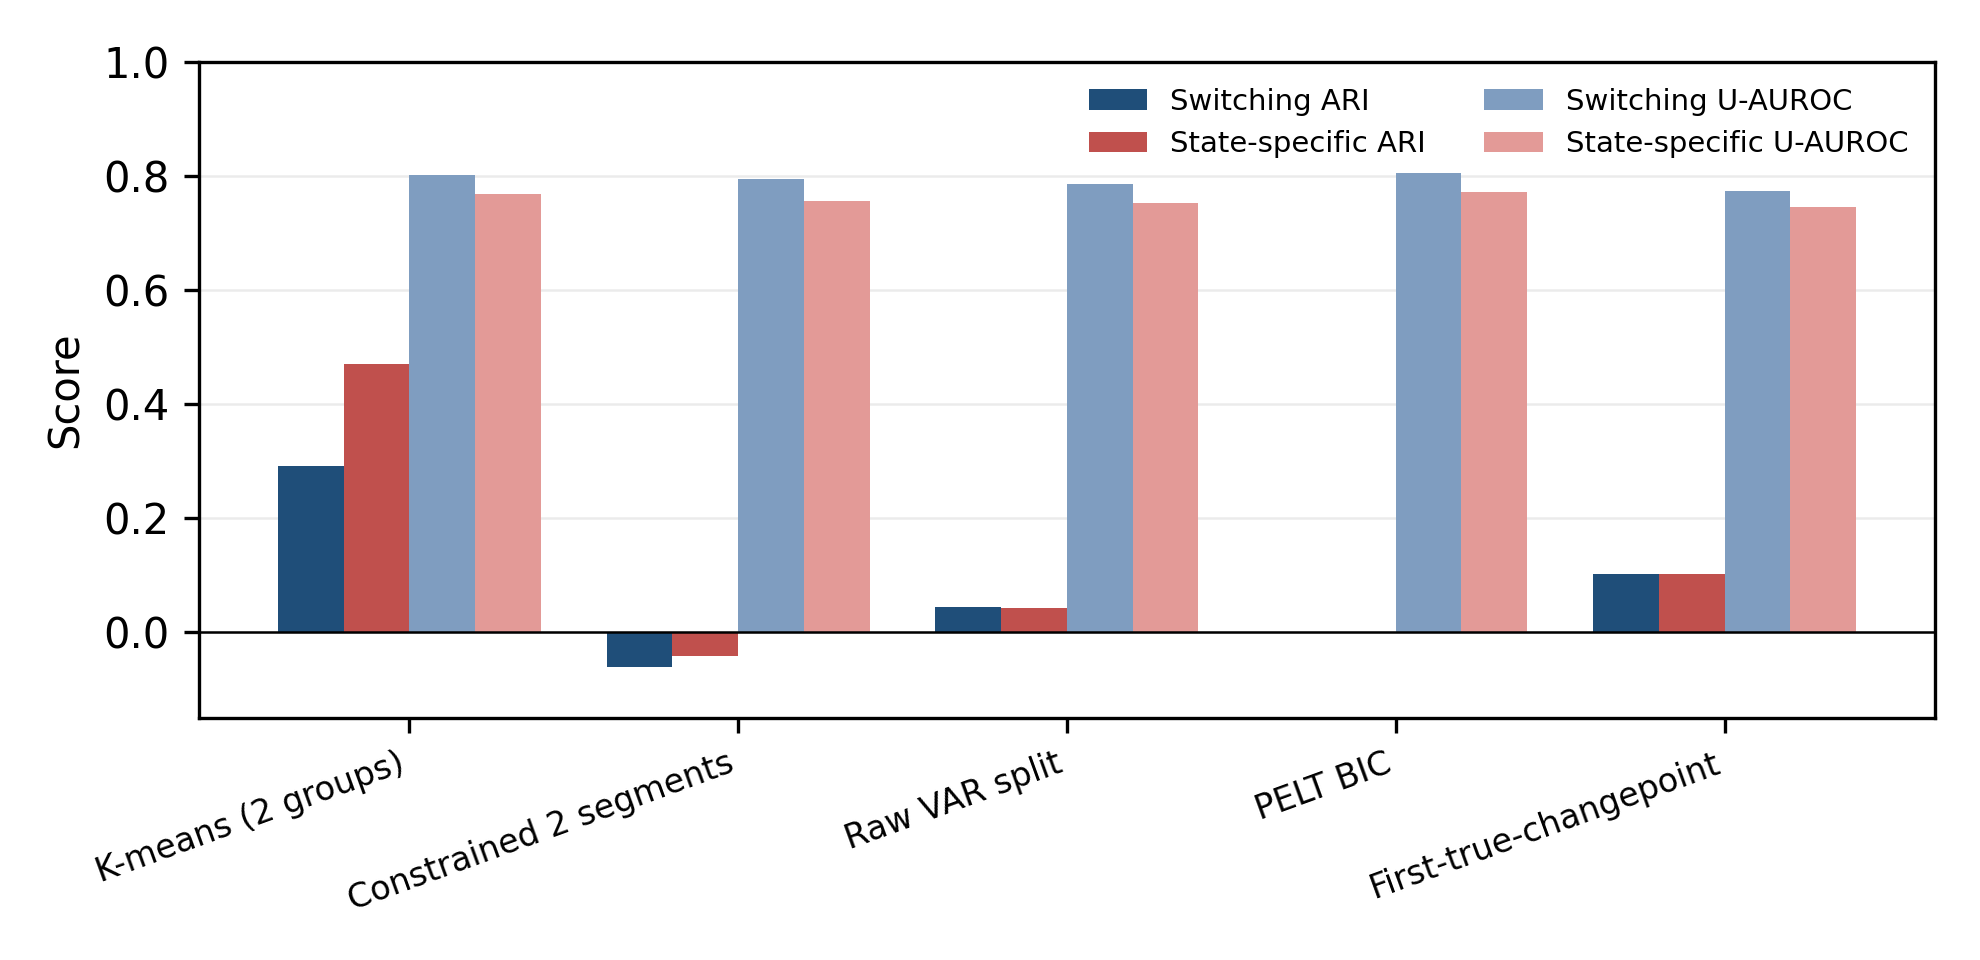
\includegraphics[width=\linewidth]{results/information_sciences/narrative_assets/rev2_segmentation.png}
\caption{State alignment and union recovery for five partitions. A fixed
two-segment model, even split at the first true change point, cannot represent
recurring regimes; union recovery is nearly the same for all of them.}
\label{fig:segmentation}
\end{figure}

\FloatBarrier
\subsection{PELT penalty and minimum-length scan}
\label{app:penalty}

Table~\ref{tab:penalty} varies the penalty multiplier from $0.25$ to $4$ and
the minimum segment length from one to three windows in the earlier
seven-window switching-core configuration, using the same twenty seeds per
cell. The mean segment counts remain $7$, $3$ and $2$
for minimum lengths one, two and three, respectively, across all tested
multipliers, so the count is controlled by the minimum-length constraint here.

\begin{table}[!htbp]
\centering
\caption{PELT on the earlier seven-window switching reference: segment counts are unchanged
across the tested penalty multipliers and depend on the minimum segment length.}
\label{tab:penalty}
\begin{tabular}{rrrr}
\toprule
Penalty factor & Min windows/segment & Mean segments & Union AUROC \\
\midrule
0.25 & 1 & 7.0 & 0.804 \\
0.25 & 2 & 3.0 & 0.799 \\
0.25 & 3 & 2.0 & 0.791 \\
0.50 & 1 & 7.0 & 0.804 \\
0.50 & 2 & 3.0 & 0.799 \\
0.50 & 3 & 2.0 & 0.791 \\
1.00 & 1 & 7.0 & 0.804 \\
1.00 & 2 & 3.0 & 0.799 \\
1.00 & 3 & 2.0 & 0.791 \\
2.00 & 1 & 7.0 & 0.804 \\
2.00 & 2 & 3.0 & 0.799 \\
2.00 & 3 & 2.0 & 0.791 \\
4.00 & 1 & 7.0 & 0.804 \\
4.00 & 2 & 3.0 & 0.799 \\
4.00 & 3 & 2.0 & 0.791 \\
\bottomrule
\end{tabular}

\end{table}
\FloatBarrier

\subsection{Auxiliary independent validation across four scenarios}
\label{supp:aux-independent-validation}
This auxiliary independent validation uses fifty seeds 3000--3049 after fixing
the method set and tests. Each seed contributes the mean over four scenarios
before inference. Its primary family compares \stcg{} with three configurations (window
max, PELT+refit and constrained two-segment refit) on union AUROC, union AUPRC
and pooled AUROC; Holm correction covers nine tests. A global
VAR-Lasso is a descriptive reference with its own interval outside that family.
This is a separate evidence block from Study A's paired-duration comparisons.
Section~\ref{app:provenance} distinguishes it from development seeds.

Table~\ref{tab:final} reports the result. \stcg{} beats all three baselines on
union AUROC and union AUPRC (AUROC gains of $+0.0109$, $+0.0382$ and $+0.0234$
against window max, PELT+refit and the constrained split; AUPRC gains of
$+0.0229$, $+0.0830$ and $+0.0398$). On the pooled AUROC target the picture is
different: \stcg{} does not significantly beat the window maximum ($+0.0021$,
Holm $p=0.42$), and its pooled-AUROC gains ($+0.042$ against the constrained
split, $+0.102$ against PELT+refit) are against two differently limited
configurations: a fixed two-segment split that under-fits the recurring
structure, and PELT, which over-segments into per-window ranges. Against the
global VAR-Lasso, no union-AUROC advantage is detected under this protocol
($+0.0006$, 95\% CI $[-0.0061,0.0071]$), while union AUPRC is lower by
$0.0206$ ($[-0.0287,-0.0128]$). The pooled-AUROC difference is $-0.0001$.
These comparisons do not establish equivalence. The pooled-AUROC advantage
over the two segmentation configurations must be read alongside their distinct
segment-count and refit limitations.

A separate within-edge temporal diagnostic on the switching-core scenario of
this fifty-seed block gives hard-minus-raw $-0.053$, with paired $95\%$ interval
$[-0.081,-0.025]$: the absolute means are $0.660$ for hard and $0.713$ for raw.
This diagnostic is not one of the nine primary cross-scenario tests.

\begin{table}[!htbp]
\centering
\caption{Auxiliary independent validation on fifty seeds (3000--3049), averaged over
four scenarios within each seed. $\Delta$ is \stcg{} minus the competitor;
intervals are seed-clustered bootstrap 95\%; Holm covers the nine primary tests.}
\label{tab:final}
\resizebox{\linewidth}{!}{\begin{tabular}{llrrrr}
\toprule
Outcome & Comparison & $\Delta$ & 95\% CI & $p_{\mathrm{Holm}}$ & Sig. \\
\midrule
Union AUROC & $-$ window max & +0.0109 & [+0.0073, +0.0146] & $<$0.0001 & yes \\
Union AUROC & $-$ PELT refit (earlier) & +0.0382 & [+0.0317, +0.0448] & $<$0.0001 & yes \\
Union AUROC & $-$ constrained refit & +0.0234 & [+0.0168, +0.0306] & $<$0.0001 & yes \\
Union AUPRC & $-$ window max & +0.0229 & [+0.0169, +0.0289] & $<$0.0001 & yes \\
Union AUPRC & $-$ PELT refit (earlier) & +0.0830 & [+0.0745, +0.0912] & $<$0.0001 & yes \\
Union AUPRC & $-$ constrained refit & +0.0398 & [+0.0307, +0.0498] & $<$0.0001 & yes \\
Pooled AUROC & $-$ window max & +0.0021 & [-0.0029, +0.0070] & 0.4176 & no \\
Pooled AUROC & $-$ PELT refit (earlier) & +0.1015 & [+0.0957, +0.1071] & $<$0.0001 & yes \\
Pooled AUROC & $-$ constrained refit & +0.0422 & [+0.0370, +0.0473] & $<$0.0001 & yes \\
\midrule
\multicolumn{6}{l}{\emph{Descriptive reference, not in the Holm family}} \\
Union AUROC & $-$ global VAR-Lasso & +0.0006 & [-0.0061, +0.0071] & -- & -- \\
Union AUPRC & $-$ global VAR-Lasso & -0.0206 & [-0.0287, -0.0128] & -- & -- \\
Pooled AUROC & $-$ global VAR-Lasso & -0.0001 & [-0.0073, +0.0066] & -- & -- \\
\bottomrule
\end{tabular}
}
\end{table}

\subsection{Fixed PELT plus graph-refit comparison on existing C inputs}
This fixed comparison is fitted on the existing central Study C inputs; it
adds an alternative segmentation/refit structure, not new independent simulation seeds.
\label{app:segmentation-validation}

PELT minimises a penalised contiguous-segment cost
\citep{killick2012optimal,ruptures_pelt_docs}; it does not infer recurrent state
identities. We apply the existing \texttt{ruptures} implementation to the
same nonself window-score features at $h=300$, stride $150$, $M=23$ in C.
Features are centred and divided by their standard deviation plus $10^{-8}$,
then projected onto the first five principal components. The cost is squared
Euclidean segment error, the penalty is fixed at $5\log(23)$,
\texttt{min\_size}=2 and \texttt{jump}=1. No true state or segment count is
supplied, and no penalty is selected from results.

Detected window boundaries map to the midpoint between neighbouring integer
window centres. The resulting half-open observed-time intervals partition
$[0,T)$ without overlap. The original short-interval merge rule requires at
least $\max(2L+5,L+3)$ samples. Each final interval is independently
standardised and refit by VAR-Lasso with $L=3$, $\alpha=0.005$, the same
self-lag regression design and nonself scoring convention. Window emissions
use the final interval containing each centre, including after merging.
Convergence warnings count as failed adapter cases; all failures, warnings,
segment maps and actual ranges would remain saved without replacement.

The 60 prelisted C cases all succeed, with 644 segment refits and no warnings.
At $D=300$, 26 repeats choose 11 segments and four choose ten; at $D=600$,
19 choose eleven, ten choose ten and one chooses nine. Thus 45 of 60 cases
reach the minimum-length maximum of eleven segments. This behaviour is
reported without retuning. The adapter changes the grouping/refit structure
but still shares the original local linear features; it is not a reproduction
of an entire published causal-discovery system.

\begin{table}[!htbp]\centering
\caption{Segmentation/refit and hard-emission contrasts against the same raw
windows in C, 30 independent paired repeats per duration. All intervals are
ordinary pointwise $95\%$ bootstrap intervals; no new hypothesis-test family
is assigned. Standard AP and method-relative F1 are not interchangeable with
the positive-change and raw-amplitude conventions. Repeated C forced-minus-raw
within-edge temporal AUROC intervals use the original Study C summaries;
other metrics retain comparison-specific streams.}
\label{tab:external-contrasts}
\resizebox{\linewidth}{!}{\begin{tabular}{rlrrr}
\toprule
$D$ & Target & Forced hard minus raw & PELT + VAR minus raw & $n$ \\
\midrule
300 & Pooled AUROC & $+0.106\;[0.098,0.114]$ & $+0.013\;[0.006,0.020]$ & 30 \\
300 & Within-edge AUROC & $-0.047\;[-0.084,-0.006]$ & $+0.005\;[-0.020,0.027]$ & 30 \\
300 & AP$_+$ & $-0.295\;[-0.386,-0.198]$ & $+0.038\;[-0.057,0.125]$ & 30 \\
300 & AP$_{\rm std}$ & $-0.037\;[-0.084,0.016]$ & $+0.169\;[0.117,0.216]$ & 30 \\
300 & F1$_{\rm raw}$ & $-0.225\;[-0.248,-0.201]$ & $+0.053\;[0.014,0.088]$ & 30 \\
300 & F1$_{\rm self}$ & $-0.036\;[-0.077,0.004]$ & $+0.065\;[0.028,0.097]$ & 30 \\
300 & Stable exceedance & $-0.005\;[-0.009,-0.000]$ & $-0.000\;[-0.002,0.002]$ & 30 \\
600 & Pooled AUROC & $+0.115\;[0.106,0.123]$ & $+0.008\;[0.001,0.014]$ & 30 \\
600 & Within-edge AUROC & $+0.037\;[0.002,0.067]$ & $-0.006\;[-0.020,0.008]$ & 30 \\
600 & AP$_+$ & $-0.055\;[-0.133,0.026]$ & $-0.125\;[-0.205,-0.044]$ & 30 \\
600 & AP$_{\rm std}$ & $+0.040\;[-0.020,0.102]$ & $-0.011\;[-0.067,0.048]$ & 30 \\
600 & F1$_{\rm raw}$ & $-0.100\;[-0.121,-0.079]$ & $-0.008\;[-0.055,0.040]$ & 30 \\
600 & F1$_{\rm self}$ & $+0.150\;[0.093,0.205]$ & $+0.008\;[-0.043,0.060]$ & 30 \\
600 & Stable exceedance & $-0.008\;[-0.011,-0.006]$ & $-0.001\;[-0.002,-0.000]$ & 30 \\
\bottomrule
\end{tabular}
}
\end{table}

\subsection{Matched-protocol computational cost}
\label{supp:runtime}
The gated hard policy, raw window maximum and PELT with window
averaging each take approximately $0.051$~s per fit; PELT with contiguous-range
refitting takes $0.063$~s. Table~\ref{tab:cost} reports these measurements on
one CPU worker under the same timing protocol.

\begin{table}[!htbp]
\centering
\caption{Wall-clock cost per fit under the same protocol, one CPU worker.}
\label{tab:cost}
\begin{tabular}{lrl}
\toprule
Method & Seconds per fit & Source \\
\midrule
Window max & 0.051 & measured \\
Gated hard & 0.051 & measured \\
PELT + refit & 0.063 & measured \\
PELT + window average & 0.051 & measured \\
\bottomrule
\end{tabular}

\end{table}

\FloatBarrier
\section{Industrial alignment and reference targets}
\label{supp:industrial}

\subsection{ESS subsystem alignment and imputation sensitivity}
\label{sec:real}

\paragraph{ESS.}
The ESS benchmark provides 227 process variables, an expert subsystem graph over
23 subsystems, and one hour of one-second data \citep{mogensen2024causal}. We
z-score each variable, average the variables inside each subsystem, and keep the
23 subsystems in the expert matrix (45 variables outside those subsystems are
dropped). We compare forward fill, backward fill, linear interpolation, and
column means. Forward and backward fill use full-hour column means for remaining
missing entries; standardisation also uses the full hour. These are offline
analyses, not strictly online imputations. Lags are collapsed by maximum before comparison
because the expert graph is rolled and not lag-specific. PELT returns $23$
segments under each imputation, each refitted on a disjoint time range without
cross-boundary lag rows. The refit mapping and its implementation correction are disclosed below. For each edge set and each null seed, $5{,}000$ graphs target the uniform
distribution over simple directed graphs with the same labelled in- and out-degrees,
excluding self-loops. The switch chain uses symmetric two-edge destination
exchanges ($90\%$) and directed three-cycle reversals ($10\%$); proposals sample
edge indices or vertices independently with replacement, not from currently
valid moves \citep{lamar2009uniform}. Rejections retain the current graph;
burn-in is $100|E|$ proposals and thinning $10|E|$. Section~\ref{app:ess-null}
specifies the proposals and reports acceptance and tail diagnostics.
Samples are shared across methods and imputations.
These are approximate finite-chain null samples, with upper-tail $p=(1+b)/5001$
for $b$ null AUROCs at least as large as observed. The plus-one formula does not
make sequential MCMC samples exchangeable or guarantee an exact finite-sample
test \citep{howes2024mcmc}. Null seeds $0$--$4$ assess
Monte Carlo variability on the same hour, with seed $0$ retained as the reference.
The forward-fill strategy remains
the primary analysis: its eight tests (four methods by two edge sets) are
Holm-corrected as one family within each seed. The other imputations are exploratory
checks; a combined $32$-test correction is also computed separately within each seed.

Table~\ref{tab:ess} reports the forward-fill result and the range over
imputations. No method exceeds $0.58$ AUROC against all expert edges in the
forward-fill result: \stcg{} reaches $0.571$, PELT $0.565$ and lagged
correlation $0.554$. On strong edges they reach $0.587$, $0.555$ and $0.677$,
respectively. At reference seed $0$, lagged correlation on strong edges has raw
$p=0.0032$ and Holm-adjusted $0.0256$. Its adjusted values span $[0.0160,0.0368]$
and remain below $0.05$ in all $5/5$ seeds; the other seven forward-fill tests
remain above $0.05$ in every seed. The all-edge \stcg{} result has reference
raw $p=0.0156$ and adjusted $0.1092$; PELT's strong-edge raw $p=0.1278$ becomes
$0.4047$. Under the combined $32$-test correction, strong-edge lagged correlation
with linear imputation has reference adjusted $0.0448$ and spans
$[0.0192,0.0512]$ ($4/5$ rejections); mean imputation rejects in only $1/5$
seeds. No combined-family rejection is stable across all five seeds.
All-edge rankings vary with imputation: \stcg{} is first under
forward fill, PELT under backward fill, and lagged correlation under linear
and mean imputation. The absolute AUROC moves by up to $0.069$ for \stcg{}.
These finite-chain degree-null results remain exploratory and do not establish
causal graph recovery or within-edge temporal discrimination. A significant
comparison to the null for one method and a nonsignificant comparison for another
do not establish a significant difference between those methods.

\begin{table}[!htbp]
\centering
\caption{ESS subsystem alignment with forward-fill imputation. Imputation range
spans AUROC over four strategies. Raw and Holm $p$ use reference seed $0$;
Holm range spans seeds $0$--$4$, each with $5{,}000$ degree-preserving null graphs
and its own eight-test forward-fill family.}
\label{tab:ess}
\resizebox{\linewidth}{!}{\begin{tabular}{llrrrrr}
\toprule
Method & Expert edges & AUROC & Imputation range & Raw $p$ & Holm $p$ & Holm range \\
\midrule
Gated hard & all edges & 0.571 & [0.528, 0.571] & 0.0156 & 0.1092 & [0.1092, 0.1316] \\
Gated hard & strong only & 0.587 & [0.518, 0.587] & 0.0322 & 0.1932 & [0.1728, 0.2208] \\
Window max & all edges & 0.545 & [0.504, 0.545] & 0.2693 & 0.5051 & [0.5051, 0.5179] \\
Window max & strong only & 0.541 & [0.518, 0.572] & 0.2525 & 0.5051 & [0.5051, 0.5179] \\
PELT + refit & all edges & 0.565 & [0.545, 0.565] & 0.1012 & 0.4047 & [0.3927, 0.4175] \\
PELT + refit & strong only & 0.555 & [0.535, 0.661] & 0.1278 & 0.4047 & [0.3927, 0.4175] \\
Lagged correlation & all edges & 0.554 & [0.554, 0.584] & 0.0460 & 0.2300 & [0.1776, 0.2300] \\
Lagged correlation & strong only & 0.677 & [0.656, 0.691] & 0.0032 & 0.0256 & [0.0160, 0.0368] \\
\bottomrule
\end{tabular}
}
\end{table}

\begin{figure}[!htbp]
\centering
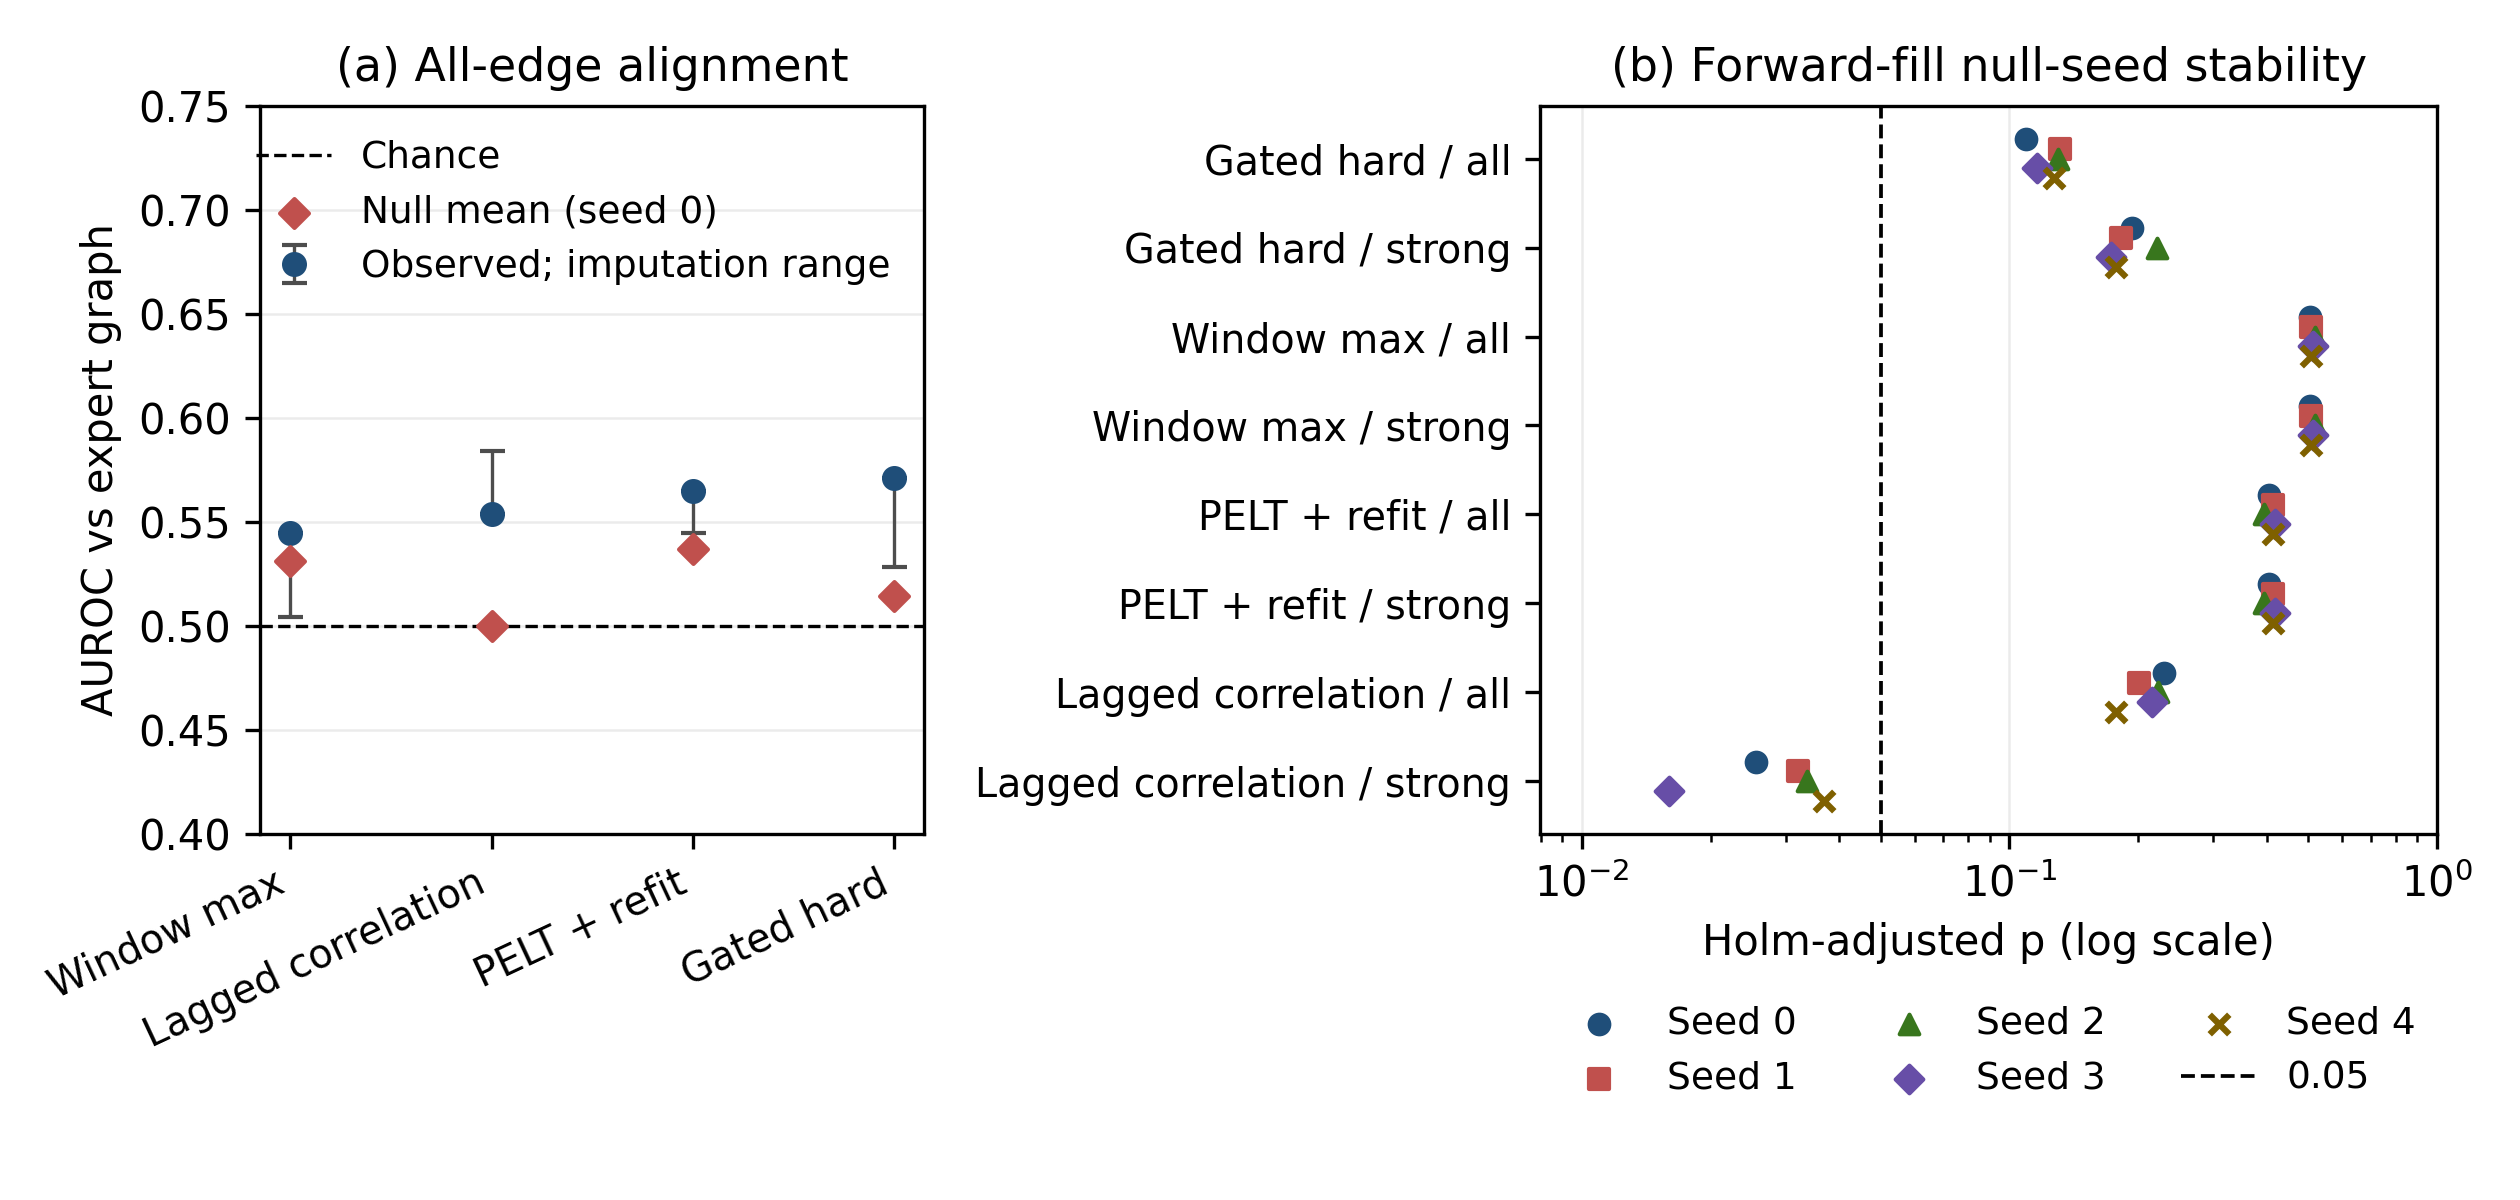
\includegraphics[width=0.98\linewidth]{results/information_sciences/narrative_assets/rev2_ess.png}
\caption{ESS alignment and null-seed stability. (a) Forward-fill all-edge AUROC:
circles are observed scores, whiskers span four imputations (not a confidence
interval), diamonds are degree-null means at reference seed $0$, and the dashed
line is chance. (b) Each marker gives one seed's forward-fill Holm-adjusted $p$
from $5{,}000$ null graphs; the dashed line marks $0.05$.}
\label{fig:ess}
\end{figure}

\paragraph{ESS contiguous-range correction.}
The ESS adapter maps adjacent window centres to half-open time ranges,
refits VAR-Lasso separately on each range without cross-boundary lag rows,
and takes the maximum score across segments and lags. Its former merge test
treated touching endpoints as overlap and collapsed all ranges. The correction
retains the $23$ ranges $[0,224),[224,374),\ldots,[3374,3600)$.
Direct global refitting reproduces the former observed AUROCs; the corrected
$200$- and $5{,}000$-draw reports have identical observed AUROCs and AUPRCs.
Thus the changed observed scores reflect the range-mapping repair, not increased
null draws. The synthetic factorial, auxiliary validation and constrained
segmentation tables use a separate refit implementation that already keeps
touching runs separate. All $24$ factorial rows at seed $0$ replay exactly;
a regression check also equates the two adapters on adequate chronological
segments. Detailed implementation records remain in the archive.

\subsection{Degree-preserving null proposals and finite-chain diagnostics}
\label{app:ess-null}

\paragraph{Target and proposals.}
The target is uniform on all loop-free simple directed graphs on the same
labelled vertices with the observed in- and out-degree at each vertex. Reciprocal
edges are allowed; parallel edges are not. Starting at the observed expert graph,
each attempted transition is:
\begin{enumerate}
\item With probability $0.9$, draw an ordered pair of edge indices independently
and uniformly with replacement. For edges $(a,b),(c,d)$, replace them by
$(a,d),(c,b)$ only if neither is a loop or already present; otherwise stay.
\item With probability $0.1$, draw an ordered vertex triple independently and
uniformly with replacement. Stay if vertices repeat. If the triple has a directed
three-cycle in either orientation and all three reverse edges are absent,
reverse it; otherwise stay. No list of currently reversible cycles is sampled.
\end{enumerate}
The reverse edge exchange has the same ordered-pair probability, since $|E|$
is fixed; each reversible triple has the same ordered-triple probability in
both orientations. Thus the kernel is symmetric, so uniform measure is
stationary without a Metropolis correction. The move types connect the fixed-degree
realisation space \citep{lamar2009uniform}; this gives no quantitative mixing-time
guarantee for these ESS chains. Every invalid proposal counts as a self-transition.

\paragraph{Diagnostics and numerical uncertainty.}
Table~\ref{tab:ess-diagnostics} replays the same five $5{,}000$-draw chains per edge
set with counters that do not consume random numbers. All ten chains reproduce
the stored lagged-correlation null means and exceedance counts. Figure~\ref{fig:ess-diagnostics}
shows complete reference traces and sample autocorrelations for this fixed score.
The tail indicator is $I_b=\mathbf1\{\mathrm{AUC}_b\ge\mathrm{AUC}_{\rm obs}\}$.
We estimate its ESS by an initial positive, monotone sequence of paired sample
autocorrelations, cap ESS at $5{,}000$, and report
$\widehat{\mathrm{MCSE}}=\sqrt{\widehat{\mathrm{Var}}(I_b)/\widehat{\mathrm{ESS}}}$.
These single-chain estimates are descriptive, especially for rare events; the
CSV additionally reports AUROC ESS and a $20$-batch means MCSE. For the reference
strong-edge chain, $b=15$, tail ESS is estimated as $5{,}000$ and MCSE as $0.00077$
(batch MCSE $0.00070$). Extending only seed $0$ to $1{,}000|E|$ burn-in gives
strong-edge raw $p=0.0022$ instead of $0.0032$. These checks reveal no marked
retained-trace dependence for the reported statistic, but neither establish
mixing nor remove finite-chain bias. Approximate $p$ and Holm values remain
exploratory; the plus-one adjustment alone provides no exact MCMC test guarantee
\citep{howes2024mcmc}.

\begin{table}[!htbp]
\centering
\caption{Lagged-correlation null-chain diagnostics. Acceptance rates are per
attempted move of that type after burn-in, including rejected proposals in the
denominator. $b$, lag-one autocorrelation $\rho_1$, ESS and MCSE concern the tail
indicator. Rows with burn/$|E|=1{,}000$ are a seed-$0$ sensitivity check, not
replacements for the primary protocol. All rows retain $5{,}000$ draws.}
\label{tab:ess-diagnostics}
\resizebox{\linewidth}{!}{\begin{tabular}{llrrrr@{\hspace{1.2em}}rrr}
\toprule
Edges & Seed & Burn/$|E|$ & 2-edge (\%) & 3-cycle (\%) & $b$ & $\rho_1$ & ESS & MCSE $\times10^3$ \\
\midrule
All & 0 & 100 & 62.94 & 0.238 & 229 & $-0.011$ & 5000 & 2.957 \\
All & 1 & 100 & 62.88 & 0.260 & 200 & $+0.026$ & 4749 & 2.844 \\
All & 2 & 100 & 62.90 & 0.240 & 222 & $+0.024$ & 4499 & 3.071 \\
All & 3 & 100 & 62.94 & 0.238 & 214 & $+0.009$ & 4888 & 2.895 \\
All & 4 & 100 & 62.94 & 0.234 & 168 & $-0.004$ & 5000 & 2.549 \\
All & 0 & 1000 & 62.98 & 0.253 & 209 & $+0.011$ & 4783 & 2.894 \\
\midrule
Strong & 0 & 100 & 73.34 & 0.042 & 15 & $-0.003$ & 5000 & 0.774 \\
Strong & 1 & 100 & 73.29 & 0.047 & 19 & $-0.004$ & 5000 & 0.870 \\
Strong & 2 & 100 & 73.26 & 0.043 & 20 & $-0.004$ & 5000 & 0.893 \\
Strong & 3 & 100 & 73.30 & 0.053 & 9 & $-0.002$ & 5000 & 0.600 \\
Strong & 4 & 100 & 73.25 & 0.048 & 22 & $-0.004$ & 4657 & 0.970 \\
Strong & 0 & 1000 & 73.26 & 0.039 & 10 & $-0.002$ & 5000 & 0.632 \\
\bottomrule
\end{tabular}
}
\end{table}

\begin{figure}[!htbp]
\centering
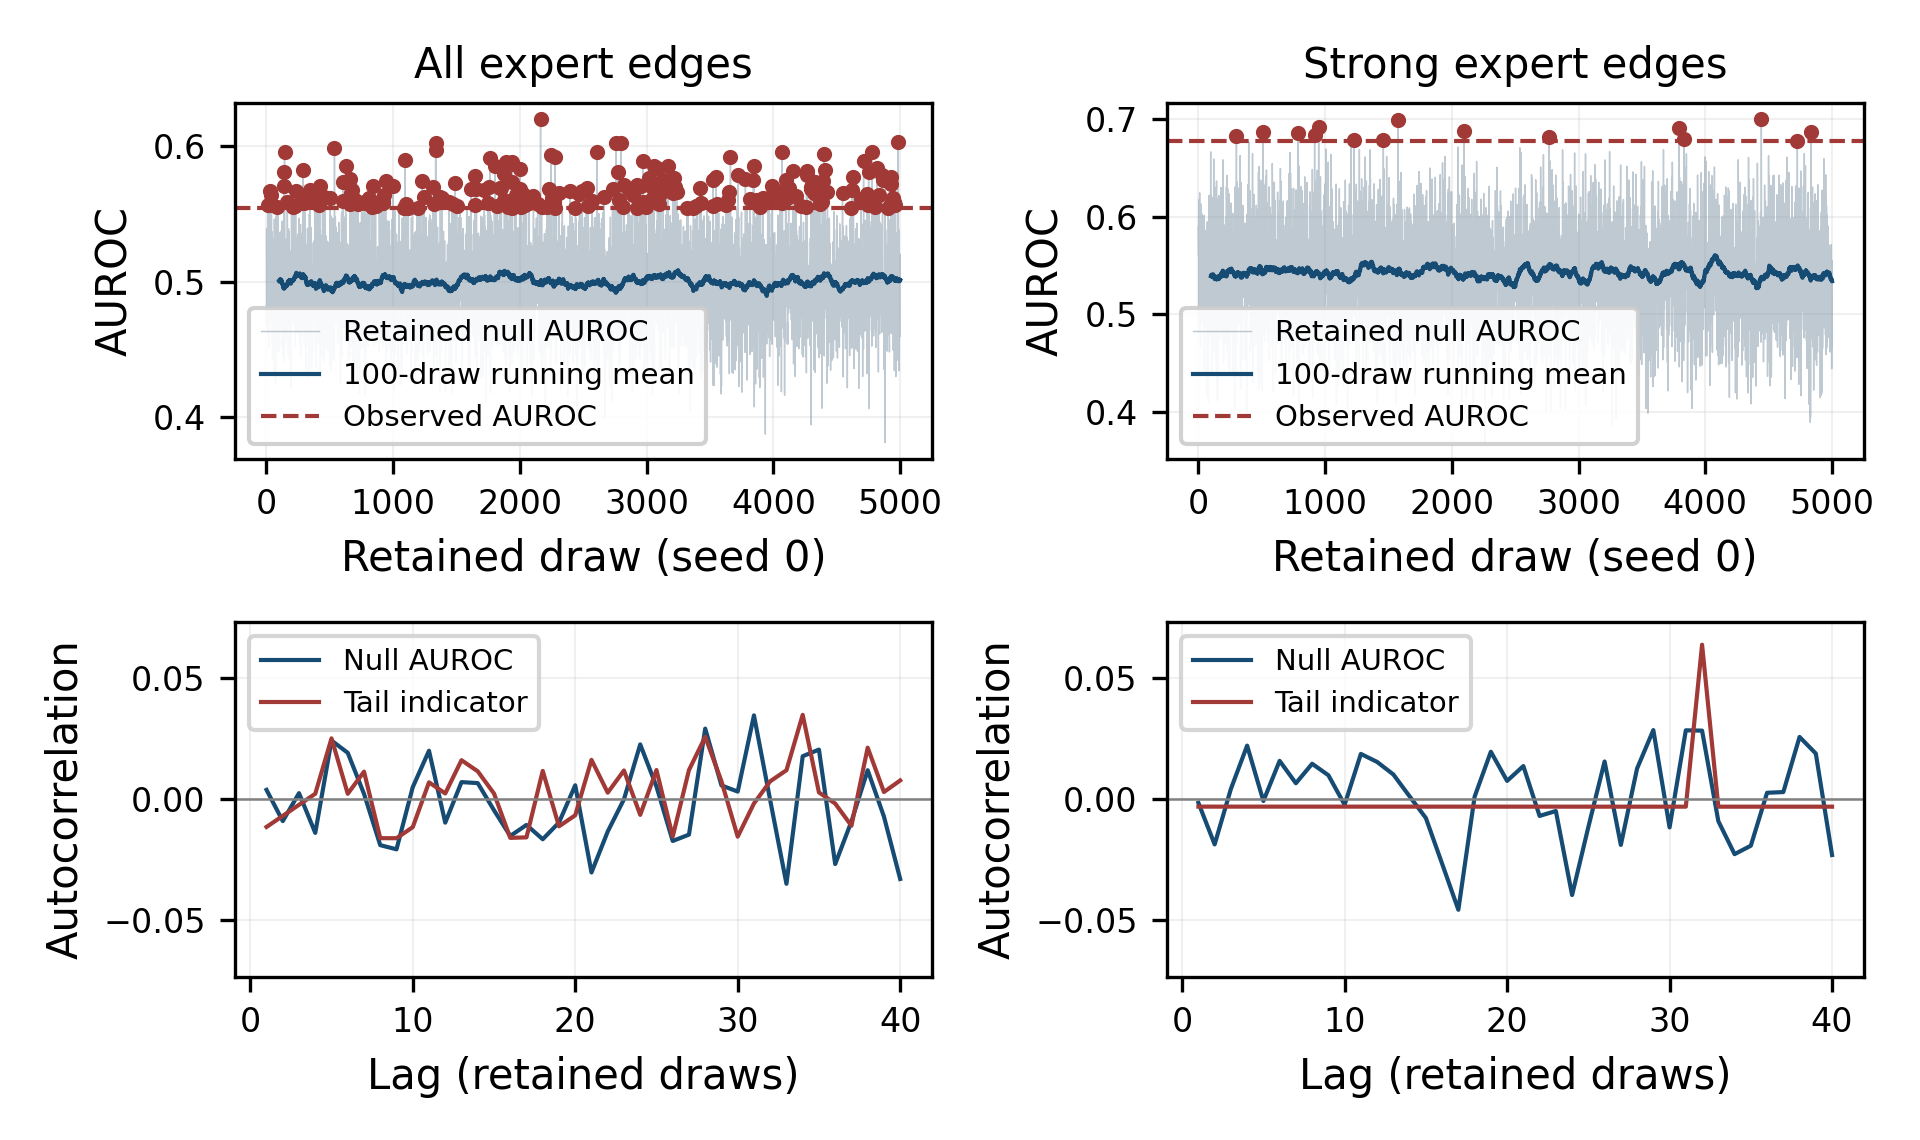
\includegraphics[width=0.98\linewidth]{results/information_sciences/narrative_assets/rev2_ess_diagnostics.png}
\caption{Reference ESS null traces (seed $0$, burn-in $100|E|$, thinning $10|E|$).
Top: all $5{,}000$ retained AUROCs, a $100$-draw running mean, and the observed
threshold; red points mark exceedances. Bottom: sample autocorrelation of the
AUROC and of its tail indicator at retained-draw lags $1$--$40$. Small empirical
autocorrelations are not a proof of adequate mixing.}
\label{fig:ess-diagnostics}
\end{figure}

\FloatBarrier
\subsection{Operating-condition labels are not graph truth}
\label{supp:operating-targets}
On HydraulicSystems and AReM, condition labels mark changes in machine settings
or activities, not changes in a stationary VAR. A change-point test calibrated on
synthetic coefficient breaks accepts $34.2\%$ of 193 Hydraulic condition
boundaries against $30.0\%$ of stable segments, and $100\%$ of both in AReM, so
those labels cannot be used as graph truth.

\FloatBarrier
\section{Reproducibility and implementation notes}
\label{supp:implementation}

\subsection{Implementation scope and analysis records}
\label{app:provenance}

\paragraph{Earlier selection and seed blocks.}
Seeds 2000--2049 were used while correcting the PELT adapter and were not treated
as an independent validation block afterwards. The fixed earlier comparison was evaluated
on seeds 3000--3049, with its own nine-test family and targets as described in
Section~\ref{supp:aux-independent-validation}. It was untouched by model selection but not a
prospectively registered sample. Neither block supplies the new independent
paired-duration replications of the main article.

\paragraph{Retained-output consistency.}
All $1{,}400$ existing hard/oracle temporal measurements and gate decisions agree
with the earlier grid, as do the $60$ core raw/hard/oracle measurements and the
$20$ historical core GMM pooled values.
The twenty-seed grid, numerical GMM sensitivity check and exact matched
grouping analysis retain their separate output records. Replaying forty old
fits to recover labels and state maps adds no seeds and does not turn the
selected-cell comparison into an independent confirmation. The earlier
responsibility-weighted GMM maps with argmax emission and the continuous-emission
variant are reported separately.

The archived original implementation is identified in code as STCG-v1.
Here its prediction rule is called gated hard, explicitly including the
static window-maximum fallback. Forced hard and raw fallback are different
emission policies with the same fitted candidate and gate decision.

\subsection{Post hoc diagnostics of saved generator outputs}
\label{app:generator-audit}
The audit reads the saved final coefficient tensors and observed trajectories;
it neither simulates missing observations nor refits a scorer.
Table~\ref{tab:generator-diagnostics} counts each independent mechanism once
for the radius range. Study A's $100$ mechanisms generate $200$ duration-specific
paths shared by Lasso and OLS; Study B's $50$ mechanisms generate $300$ paths.
All $500$ saved observed paths are finite. The maximum absolute observed values
are $0.532854$ and $0.555313$ in A and B. The endpoint ratio is the RMS of all
nodes in the final $300$ observed samples divided by the RMS in the first
$300$. Its ranges are $[0.930770,1.050883]$ and $[0.936157,1.063834]$.
These are post hoc descriptive checks with no prespecified stability cutoff;
the endpoint ratio is not a fitted growth rate and never controls inclusion.

Saved observations cover full-time intervals $[100,1300)$ in A and
$[100,3700)$ in B. The original simulator checks finiteness before dropping
burn-in; this independent audit examines only the saved post-burn-in series.
It does not reconstruct the missing $100$ burn-in observations. Pre-rescaling
radii were not saved, so the number of applied rescalings is not inferred from
final radii alone. Finite observed paths and state-wise radii do not establish
general stability under arbitrary switching.

State $A$ has no self support. State $B$ self-edge counts span $0$--$7$ across Study A
mechanisms and $0$--$6$ across Study B mechanisms. Realised shared/A support
fractions span $[0.281,0.742]$ and $[0.333,0.706]$, rather than equalling $0.5$
in every draw. The retained supports exclude activation of either empty-support
safeguard in these $150$ mechanisms. Full per-mechanism and per-path diagnostics
are in \path{results/information_sciences/generator_audit/}; its manifest binds
the audit tool, outputs and unchanged frozen-source snapshots.

\begin{table}[!htbp]
\centering
\caption{Post hoc diagnostics of retained generator outputs. Radius ranges
use final companion matrices; paths are paired within mechanism and are not
independent mechanism replicates. RMS uses the first/last 300 saved observed
samples and all nodes. No numerical cutoff or sample selection is introduced.}
\label{tab:generator-diagnostics}
\resizebox{\linewidth}{!}{\begin{tabular}{lrrrrrr}
\toprule
Study & Mechanisms & Paths & Actual radius range & Max $|X|$ & Late/early RMS range & Finite paths \\
\midrule
A & 100 & 200 & [0.381, 0.676] & 0.533 & [0.931, 1.051] & 200/200 \\
B & 50 & 300 & [0.404, 0.627] & 0.555 & [0.936, 1.064] & 300/300 \\
\bottomrule
\end{tabular}
}
\end{table}

\subsection{Selected same-seed generation and fitting checks}
\label{app:fresh-checks}
We separately regenerate and fit A seeds 50000--50001 and C seeds 70000--70001
at both durations, eight selected pipeline cases. RNG inputs and trajectories
are generated anew and saved before fitting; fitted arrays are not used to
initialise the reruns. The isolated environment matches the 47 pinned
dependencies. All 228 array comparisons, 132 original-metric comparisons and
132 recomputed-metric comparisons are exact on this machine, rather than
merely within the predeclared $10^{-10}$ relative/$10^{-12}$ absolute
tolerance. These existing-seed reruns test the selected pipelines; they do
not add independent seeds, test every setting from scratch or constitute an
independent algorithm implementation.

The existing-output sensitivity analysis and the fixed segmentation/refit
comparison have source/input/output hash closures and internal execution
records, with no public-preregistration claim. The archive includes the
fixed protocols, per-case arrays, summaries and evidence index. Its read-only
entry point recomputes saved-output metrics and intervals without fitting;
the display-rebuild route reconstructs figures and tables. New generation
and fitting require an explicit new destination and are documented separately.
The complete archive is available for review in
the versioned public release identified in Section~\ref{app:reproduction}.

\subsection{Access, cached replay, and rebuilding}
\label{app:reproduction}
The companion archive \path{information_sciences_reproducibility.zip}
contains manuscript sources, configurations, retained inputs, emissions,
assignments, truth, per-repeat results and presentation builders. Version
\texttt{v2026.10.27} is available at
\url{https://github.com/xschang1002/latent-state-graph-recovery/releases/tag/v2026.10.27}.
Its root README gives environment setup, data-access
requirements and the execution index. The basic entries are:
\begin{quote}\small\ttfamily
python scripts/reproduce\_paper.py --verify\\
python scripts/reproduce\_paper.py --rebuild
\end{quote}
Verification recomputes metrics, intervals and provenance from retained outputs
without fitting or writing. Rebuild regenerates deterministic retained-output
analyses and presentation files; it does not generate a new simulation sample.
The separately documented simulation/fitting entries require frozen protocols
and a new destination. Adding \texttt{--compile} uses an installed TeX engine.
Public industrial datasets used by older auxiliary protocols may require
separate acquisition, as distinguished from the packaged data in the README.

The machine-readable evidence index and research guide locate every study's
protocol, per-case arrays, comparison families, missing-target coverage,
source/output hashes and replay commands. Detailed historical script lists,
development sequence and clock records remain in the repository rather than
serving as evidence of new independent experiments. The earlier risk, occupancy,
Brier, selection and pooled-refit probes are mechanism illustrations and are
not pooled with the simulation-study tables. Internal source-lock times and
filesystem observations are distinguished from externally attested registration;
no public-preregistration claim is made.

\bibliographystyle{plainnat}
\bibliography{paper/references}
\end{document}
